\documentclass[10pt]{article} % 10pt 字体大小,单栏布局
%\documentclass[10pt,journal]{IEEEtran}
\usepackage{ctex}          % 支持中文
\usepackage{fontspec}      % 允许自定义英文字体(适用于 XeLaTeX 或 LuaLaTeX)
\usepackage{cite}
\usepackage{amsmath,amssymb,amsfonts}
\usepackage{graphicx}
\usepackage{booktabs}
\usepackage{geometry}
\usepackage{subcaption}
\usepackage{makecell}      % 竖排换行
\usepackage{placeins}
\usepackage{setspace}
\usepackage{titlesec}
\usepackage{tikz}
\usepackage{adjustbox}
\usepackage{float}
\usepackage{booktabs, multirow, xcolor}  % 你若已有就不用重复
\usepackage{siunitx,enumitem}
\usepackage{bm}        % 提供 \bm
\usepackage{booktabs}
\usepackage{pifont}        % 五角星符号
\usepackage{caption}
\usepackage{subcaption}
\usepackage[normalem]{ulem}
\newcommand{\placeholder}[1]{\textcolor{red}{#1}}
\usetikzlibrary{shapes.geometric, arrows, positioning}
\usepackage[ruled,vlined]{algorithm2e} % 算法格式支持
 

% 页面布局设置
\geometry{a4paper, left=0.5in, right=0.5in, top=1in, bottom=1in} % 减小页边距

% 标题格式设置
\titleformat{\section}{\large\bfseries}{\thesection\ }{0em}{} % 一级标题无点
\titleformat{\subsection}{\normalsize\bfseries}{\thesubsection\ }{0em}{} % 二级标题无点
\titleformat{\subsubsection}{\normalsize\bfseries}{\thesubsubsection\ }{0em}{} % 三级标题无点

% 行距设置
\setstretch{1.2} % 行距 1.2 倍

% 公式编号统一格式
\numberwithin{equation}{section}

\begin{document}

\title{\textbf{数据清洗与下游聚类的自动化协同优化及其影响机理研究}}
\date{\today}
\maketitle

% 摘要部分
\noindent\textbf{\large 摘要}\\
在许多无监督学习任务中,现有的数据清洗与聚类技术已能在一定程度上降低噪声与缺失值带来的影响,但仍难以同时兼顾多样化清洗策略与聚类算法在大规模、高维数据中的协同需求。为进一步提升聚类质量与自动化效率,本文提出了一种清洗-聚类协同优化框架:通过多标签学习模型将数据的特征向量映射到最优或近优的“清洗-聚类”管线组合,从而在大幅减少搜索空间的同时确保较高的聚类性能。在提供解决方案的同时,我们还系统地分析了清洗对聚类算法运行及评价指标的影响,并通过清洗准确度与聚类指标的关联性研究,揭示了在不同数据特征与错误率下清洗策略对聚类收益的关键影响因素。基于对 60 个公开数据集的大规模实验发现,不同数据特征会显著影响清洗与聚类的适配性,例如 Raha-Baran + HC 组合在高维、多特征数据上较为稳健,而 mode + DBSCAN 在低维数值数据上对噪声表现出极端敏感。通过该框架的自动化推荐与筛选,在部分场景下实现了平均 5.83 倍的搜索加速,并在保证聚类质量的同时取得了 19.20\% 的平均提升率。研究结果表明,该方法对多样化数据具有一定的稳健性与可扩展性,为噪声较高、规模较大的真实数据环境提供了切实可行的聚类优化方案。


\section{引言}

在大数据与人工智能的快速发展背景下,无监督学习(如聚类分析)在医疗、金融及工业物联网等众多领域发挥着日益重要的作用\cite{Aljohani2024, 10729915, Passlick2021}。例如,在医疗场景中,通过聚类可从病患数据中挖掘潜在群组,为个性化诊疗提供决策支持\cite{10.1007/978-3-031-72506-731};在金融场景中,聚类方法可以帮助区分用户信用类别、增强客户预期回报的信心等\cite{Cai2016}。已有研究在聚类算法改进和可视化等方面取得了显著成果,常用的方法包括 K-Means 及其变体\cite{Bandyapadhyay2024}、基于密度的 DBSCAN 以及层次聚类、图聚类\cite{10.1145/3299876}等,这些方法为不同数据形态提供了有效的划分策略。与此同时,数据清洗技术(例如缺失值填补、异常值检测、错误值纠正)也在学术界与工业界获得广泛应用,用以降低噪声影响和提高数据质量\cite{10.1145/2723372.2749431, 10.1145/2463676.2465327, Rekatsinas2017}。

然而,在无监督学习场景中,数据质量的影响往往更为突出。与分类或回归等有监督学习相比,聚类对于数据分布的依赖更强,一旦噪声、缺失值或错误值的比例较高,就可能破坏簇结构与真实分布之间的对应关系\cite{ALAM2023100341},从而对模式挖掘和决策支持造成不可忽视的干扰。虽然已有清洗方法在减少噪声方面效果显著,但过度或不当的清洗有时反而扭曲了关键特征\cite{Ni2023};此外,不同的聚类算法对数据缺陷的敏感度各异\cite{SINGH2024102799},若仅侧重于数据清洗或聚类算法单方面的优化,往往难以协调两者之间的相互作用,从而难以获得整体最优的策略。

为解决上述问题,研究者逐步认识到“清洗策略 + 聚类算法 + 超参数”一体化管线的重要性\cite{Blumenberg2020}。这种做法能在保证数据分布尽量真实的同时,为不同数据集的特性“量体裁衣”地提供最佳策略。但由于管线搜索空间常呈指数级增长,且无监督场景缺乏显式标签指导,仅靠人工穷举或简单试验往往难以在可接受时间内完成参数寻优。近年来,自动化机器学习(AutoML)在有监督学习领域已呈现出显著优势\cite{Barbudo2023},不仅能自动选择模型结构及超参数,还能优化特征工程\cite{SALEHIN202452, HE2021106622}。然而,大部分 AutoML 研究集中于分类或回归任务\cite{9458702},对无监督学习特别是“清洗+聚类”协同自动化的探索仍相对有限\cite{10.1145/3643564}。这为我们带来了新的机遇与挑战:能否将数据质量与无监督聚类的协同优化思路融入 AutoML 框架,并结合更深层次的机理剖析,在大规模及多场景下实现高效且可解释的自动管线搜索。

在此过程中, 深度理解清洗操作如何影响下游聚类算法至关重要: 只有梳理清楚清洗对聚类影响的机制和环节, 才能在自动化管线中有针对性地选择或组合清洗策略与聚类方法。为此,我们将清洗的影响拆分为四个关键层面:\textbf{(1)}~清洗对数据集准确度的影响(具体表现在对错误的修复程度),\textbf{(2)}~清洗对聚类算法内部过程的干预(如迭代收敛路径、核心点判定),\textbf{(3)}~清洗对聚类结果指标(如 Silhouette、DB 指数)的影响,\textbf{(4)}~清洗对聚类超参数选择(如 K-Means 的 $k$ 值、DBSCAN 的 $\varepsilon$)的影响。通过从“源数据集—算法运行过程—聚类指标—超参数调优”四步逐层深入地分析,我们不仅能更好地解释清洗策略与聚类性能之间可能存在的因果关联,也为自动化管线的配置与调优提供了更丰富的理论支撑。

基于上述背景与需求,本文针对“数据清洗与下游聚类协同优化”这一交叉方向,提出了一种新的自动化管线模型,并进一步从理论层面对“清洗操作如何影响聚类”展开深度剖析:一方面,借助多标签学习模型将多种清洗策略、聚类算法及其超参数统一纳入搜索空间,在离线阶段学习“数据特征到优选方案”的映射关系;另一方面,系统研究清洗准确度与聚类评价指标之间的关联,为理解清洗操作如何干预聚类运行过程及结果指标提供实证依据。这样,当面对新的数据集时,系统能快速推荐若干最优或近优组合,大幅缩减搜索规模,并根据清洗机理的分析获得更全面的可解释性与稳定性。

\textbf{本研究的主要贡献包括:}
\begin{enumerate}
    \item \textbf{系统性地评估“清洗策略 × 聚类算法”组合的协同表现}

    基于 60 个具备多元质量问题的公开数据集,我们深入研究了不同噪声水平、错误率及规模下的 8 种清洗策略和 6 种聚类算法,对其组合在聚类质量、极端案例和时间开销方面进行了量化与比较。该评估不仅提供了对现有清洗-聚类方案适配度的系统认识,也为后续管线设计提供了实用参考。

    \item \textbf{提出基于管线思维的协同优化框架}

    将“数据清洗 + 聚类 + 超参数”作为一个整体管线(Pipeline),并结合实验结果总结出多种针对性建议,帮助研究者在实际场景中有的放矢地进行策略选择,避免仅在单一端的优化而忽略全局效果。

    \item \textbf{构建并验证了一个完整的自动化管线优化模型}

    我们引入多标签学习来捕捉“数据特征与最优清洗-聚类组合”之间的关系,大幅减少了管线搜索空间。在多个数据集上验证表明,自动化模型通常可获得 $3\times$ 以上的加速,同时保持较高的聚类准确度,证明了将 AutoML 思路拓展到无监督学习领域的可行性与有效性。

    \item \textbf{从理论角度剖析清洗对聚类的影响机理}

    通过对清洗准确度(EDR、Precision、Recall、F1)与聚类评价指标(Silhouette、DB、Combined Score)的关联研究,系统揭示了不同数据特征和错误率水平下清洗操作如何影响聚类过程,从而为参数调优与动态适配提供了更深层次的参考。

    \item \textbf{为多样化数据场景的聚类优化提供可迁移路径}

    通过对损失率、加速比等指标的度量,我们量化了自动化管线在平衡质量与效率方面的潜力,为工业领域部署该思路奠定了实践基础,也为研究者进一步探索清洗与聚类协同优化的动态适配、在线更新等提供了方向。

    \item \textbf{\textcolor[rgb]{0.00,0.07,1.00}{按错误类型细粒度量化清洗对聚类的收益,并将该洞察用于改进 AutoML 搜索策略}}

    \textcolor[rgb]{0.00,0.07,1.00}{本文首次在大规模实验中,将缺失、格式错误、离群值等不同错误类型对聚类流程的影响拆解分析;并把这些类型-级指标注入多标签学习模型,以动态收缩搜索空间,从而进一步提升 AutoML 推荐的精度与效率。}
\end{enumerate}

\textcolor[rgb]{0.00,0.07,1.00}{
我们的工作不仅加深了无监督场景下 “数据清洗—聚类” 协同机理的理解,也为自动化机器学习(AutoML)在脏数据环境中的落地探索了新路径。全文结构如下:第 2 章回顾相关工作;第 3 章形式化地定义问题与符号;第 4 章给出清洗与聚类协同的实现框架;第 5 章以 40 个数据集的大规模实验归纳宏观现象;第 6 章则进一步结合各清洗算法原理,对过程指标与错误类型做细粒度机理分析,并将结论嵌入 AutoML 搜索空间以完成强化验证。}


%---------------------------------
% 第二章:相关工作
%---------------------------------

\section{相关工作}\label{sec:related_work}

为了更深入理解“清洗策略与聚类算法协同优化”在不同场景下的研究现状,本文从以下三个方面回顾相关工作:首先,探讨数据清洗与数据质量管理的相关方法;其次,分析主要聚类算法的原理及其优化思路;最后,梳理自动化机器学习(AutoML)在无监督学习场景中的研究进展与应用探索。

\subsection{数据清洗与数据质量管理}
数据清洗旨在识别并修复各种数据缺陷(如缺失值、噪声、重复记录或错误值),是提升数据整体质量的重要途径,已有研究在统计方法和机器学习方法方面均取得了丰富成果。例如,早期工作主要依赖众数/均值填补\cite{10.1093/bioinformatics/btr597}或规则驱动的异常值检测\cite{6544854, 5767833},在处理缺失值和简单错误时比较高效;后续研究则引入高级方法,如概率图模型\cite{9151362},主动学习\cite{10.14778/2994509.2994514, 10.1145/3357384.3358129},神经网络\cite{Krishnan2017}等,以应对更复杂的错误类型。部分工作还引入了上下文约束或知识图谱\cite{6544847,10.14778/3407790.3407801},对特定领域(如医疗、经济数据)的不一致或罕见值进行更有针对性的纠正。

与此同时,研究者也认识到过度或不当清洗可能使原本有价值的异常点被误删或被扭曲\cite{Ni2023}。在有监督学习场景下,数据清洗常可借助标签对比来区分“真正有意义的异常”与“噪声性错误”\cite{Bernhardt2022};然而在无监督场景中,缺乏标签指导,清洗策略一旦过于保守或激进,就会对后续的聚类分析产生不可预测的影响。这些研究进展表明,数据清洗方法的选择与配置应当与下游分析任务(如聚类)紧密结合,而非单独孤立地追求“最干净”的数据\cite{Hu2017}。这也为我们随后探讨的“清洗与聚类协同优化”提供了重要动机。

\subsection{聚类算法及其改进}
聚类作为典型的无监督学习方法,已在图像识别、文本挖掘、用户分群等领域中得到了广泛应用。现有聚类算法大体可分为基于质心(如 K-Means 及其变体\cite{Bandyapadhyay2024, HUANG2021107996, IKOTUN2023178})、基于密度(如 DBSCAN\cite{Abdulhameed2024, CHENG2024120731},OPTICS\cite{HAJIHOSSEINLOU2024126094, 10.3233/IDA-205497, KAMIL20232625})与层次聚类\cite{CHEN2025125714}三类。不同算法在簇形状、噪声耐受度、计算复杂度等方面各具优势\cite{SINGH2024102799}。

在面对不完美数据时,上述聚类算法往往对异常值和缺失值表现出不同的敏感度。例如,少量异常点被 K-Means 视为远离中心的“噪声”,可在重新计算均值时抵消\cite{Atif2024};但若这些点在 DBSCAN 的邻域定义中被错误识别,就可能导致过度分割\cite{Guo2024}。部分工作试图在算法内部引入鲁棒性机制,如改进距离度量或引入加权方案\cite{8896034},但大多仍需事先对数据进行相对独立的预处理,缺乏将“清洗策略”与“聚类算法”放在同一管线中统筹考量,在更复杂的高噪声场景中难以取得较好的聚类结果。

\subsection{AutoML 与无监督场景的探索}

近年来,AutoML 框架(如 Auto-sklearn\cite{10.5555/3586589.3586850}、TPOT\cite{Olson2019, Romano2021}、H2O AutoML)已在有监督学习任务(分类、回归)中展现出卓越的自动化建模与超参数优化能力。典型方法主要依赖贝叶斯优化、遗传算法\cite{10.1145/3674029.3674058}等技术,在预定义的搜索空间内高效探索最优模型配置。然而,这些框架主要针对有监督任务设计,难以直接适用于无监督学习,尤其在聚类任务中面临诸多挑战\cite{10.1145/3643564}。在少量试图探索 AutoML 在无监督学习上应用的研究中(表~\ref{tab:aml_clustering_summary}),其方法主要聚焦于聚类算法选择与超参数优化,部分工作结合初步聚类或 PCA 降维以降低特征噪声。

\begin{table}[t]
\centering
\small
%\begin{adjustbox}{width=\linewidth}
\begin{tabular}{lcc}
\toprule
\textbf{方法} & \textbf{是否包含数据清洗} & \textbf{是否端到端 AutoML 模型} \\
\midrule
AutoClust\cite{9338346}          & $\times$ 无                  & $\times$ 仅聚类优化 \\
cSmartML\cite{9671542}           & $\times$ 无                  & $\times$ 仅算法选择+超参数优化 \\
MARCO-GE\cite{10031201}          & $\triangle$ 部分(PCA)      & $\times$ 主要关注算法推荐 \\
AutoCluster\cite{10.1007/978-3-030-75768-720} &
                                  $\times$ 无                  & $\triangle$ 部分端到端(集成学习) \\
TPE-AutoClust\cite{10031132}     & $\triangle$ 部分(初步聚类) & $\triangle$ 部分端到端(优化 + 集成) \\
\textbf{本文方法}                & $\checkmark$ 完整数据清洗   & $\checkmark$ 端到端自动化管线优化 \\
\bottomrule
\end{tabular}
%\end{adjustbox}
\caption{当前无监督 AutoML 聚类主要方法对比}
\label{tab:aml_clustering_summary}
\end{table}

\textcolor[rgb]{0.00,0.07,1.00}{然而,现有研究在“清洗-聚类-AutoML”闭环上仍\textbf{缺少系统化建模与量化}:
\begin{itemize}[nosep,leftmargin=*]
    \item 多聚焦于聚类算法推荐 + 超参数搜索,而数据特征如何驱动最优清洗-聚类组合缺乏定量分析;  
    \item 评估侧重最终 Silhouette/DB 等结果指标,而忽略“清洗 $\rightarrow$ 聚类内部过程”(质心收敛、核心/边界判定等)的干预链路;  
    \item 尚无完整的端到端整合清洗、聚类与调参的无监督 AutoML 框架,难以应对高噪声、多特征、错误类型交叠的数据场景。  
\end{itemize}}

\subsection{小结与差异}
\label{subsec:summary-related}

\textcolor[rgb]{0.00,0.07,1.00}{数据质量管理与聚类算法各自已形成成熟体系,AutoML 在有监督学习中也愈趋完善;\textbf{但在无监督情形仍存在以下不足:}
(i) 缺乏可端到端联动“清洗 + 聚类 + 超参数”的自动化框架;
(ii) 现有无监督 AutoML 未将\emph{清洗准确度及错误类型特征}纳入搜索维度;
(iii) 清洗-聚类在多错误类型叠加场景下的协同机理尚无系统量化。}

\medskip
\textcolor[rgb]{0.00,0.07,1.00}{
为了改进上述不足,本文提出\emph{基于多标签学习的管线化 AutoML 框架},核心思路如下:  
\begin{enumerate}[nosep,leftmargin=*]
  \item \textbf{统一搜索空间}——将“数据清洗策略 $\times$ 聚类算法 $\times$ 超参数”整体建模,通过离线多标签学习,学习“数据特征 $\rightarrow$ 优选组合”映射,显著裁剪候选子空间;  
  \item \textbf{过程级记录}——在线阶段细粒度追踪错误类型级清洗准确度(缺失、离群、格式错误等)与聚类运行轨迹(迭代步数、质心位移、核心点变化等),实现清洗收益的因果量化;  
  \item \textbf{原理驱动反馈}——结合各清洗算法原理,分析其在不同错误模式下对聚类的优势与局限,并将所得启示动态反馈至 AutoML 搜索策略,从而持续优化搜索效率与聚类质量。  
\end{enumerate}
该框架为回答“清洗何时、如何、在多大程度上提升下游聚类”提供了系统化解决方案,也为无监督 AutoML 的落地实践给出可复制的改进路径。}

%---------------------------------
% 第三章:问题定义与挑战
%---------------------------------
\section{问题定义与挑战}
\label{sec:problem-and-model}

\textcolor[rgb]{0.00,0.07,1.00}{}在第~\ref{sec:related_work} 节回顾了数据清洗、聚类算法及 AutoML 的研究进展后,我们发现:尽管各自领域已有丰富成果,但在“高维、多源、噪声与缺失并存”的真实场景中,数据清洗与聚类执行并非简单串联——二者在数据分布、算法收敛路径及超参数选择上存在深度耦合,直接影响最终聚类效果。为实现真正的端到端自动化优化,我们需首先构建一个统一的数学模型,将“清洗操作→数据分布变化→聚类内部过程→最终评价”作为一个整体加以刻画。


\subsection{数学模型与形式化定义}\label{subsec:formal-definition}

为在理论与应用中更好地理解并解决“数据清洗与聚类算法”的协同优化,本小节对核心概念进行形式化定义,并建立相应的评价体系。

\subsubsection{核心概念与变量定义}
\label{subsec:core-def}
%--------------------------------------------------
\textcolor[rgb]{0.00,0.07,1.00}{
设待处理数据集记为 \(D\)。  
其单元格可能同时含有多种脏污类型;本文用  
\(\mathcal{T}\!=\!\{\text{Missing},\text{Anomaly},\text{Typo},\dots\}\)  
表示完整的“错误类型”集合,其中的约束条件是:  
\emph{缺失值(Missing)与其他类型互斥}——因为一旦某个单元格为空值,就不会再出现其他错误信息。}

\vspace{0.3em}
\paragraph{\textcolor[rgb]{0.00,0.07,1.00}{理论特征向量}}
\textcolor[rgb]{0.00,0.07,1.00}{对任意 \(t\!\in\!\mathcal{T}\) 记
\(r_t(D)\in[0,1]\) 为该类型在 \(D\) 中的\emph{边际比例};  
再用对称矩阵 \(\mathbf{C}(D)\in\mathbb{R}^{|\mathcal{T}|\times|\mathcal{T}|}\)  
描述不同类型在同一单元格中“共现”的二阶比例,
其中 \(\mathbf{C}_{ij}=P(\text{err}_i\land\text{err}_j)\)。
若 \(t=\text{Missing}\) 或 \(i=\text{Missing}\vee j=\text{Missing}\) 则  
\(\mathbf{C}_{ij}=0\)。记总观测脏污率
\(\mathrm{ErrorRate}(D)=\sum_{t}r_t-\sum_{i<j}\mathbf{C}_{ij}\)。  
综合得到\footnote{%
在实现中可仅存上三角元素 \(\mathrm{vec}(\mathbf{C})\),
以免维度冗余;此处写成完整形式便于阅读。}  
\begin{equation}\label{eq:xD}
  \mathbf{x}_{\mathrm{gen}}(D)=
  \Bigl(
     \mathrm{ErrorRate}(D)\,;\,
     r_{t_1}(D),\ldots,r_{t_{|\mathcal{T}|}}(D)\,;\,
     \mathrm{vec}(\mathbf{C}(D))\,;\,
     m,n
  \Bigr),
\end{equation}
其中 \(m,n\) 分别为特征维度与样本规模。该向量既统一刻画了\textbf{规模}
又保留了\textbf{错误异质性},是后续多标签自动化模型
\(\Phi:\mathbf{x}(D)\mapsto\Omega'(D)\) 的输入。}


记 \(\mathcal{C}\) 为数据清洗方法的集合(如缺失值插补、异常值剔除、错误值纠正等),\(\mathcal{H}\) 为聚类算法集合(如 K-Means、DBSCAN、层次聚类等),\(\mathcal{P}\) 为聚类算法的超参数空间。将一个具体的清洗方法 \(c\)、聚类算法 \(h\) 及其超参数 \(\boldsymbol{\theta}\) 组合成\textbf{清洗-聚类策略}:
\begin{equation}\label{eq:omega}
  \omega 
  \;=\; 
  \bigl(c,\; h,\; \boldsymbol{\theta}\bigr),
\end{equation}
所有可行策略的笛卡尔积构成初始搜索空间:
\begin{equation}\label{eq:Omega}
  \Omega 
  \;=\; 
  \mathcal{C} \;\times\; \mathcal{H} \;\times\; \mathcal{P}.
\end{equation}
此时,如何在如此庞大的 \(\Omega\) 中高效找到适配度高的\(\omega\) 即是后续的研究重点。

\subsubsection{评价系统与最优方案}
为了准确衡量任意策略 \(\omega \in \Omega\) 在数据集 \(D\) 上的聚类质量(或适配性),通常采用若干无监督评价指标加以综合。本文主要使用Davie-Bouldin(DB)指数\cite{4766909}与轮廓系数(Silhouette)\cite{ROUSSEEUW198753}这两类典型指标,并线性组合为\textbf{综合得分}:
\begin{equation}\label{eq:S-score}
  S(D,\omega)
  \;=\;
  \alpha \cdot \bigl[-\,DB(D,\omega)\bigr]
  \;+\;
  \beta \cdot \mathrm{Sil}(D,\omega),
\end{equation}
其中 \(\alpha,\beta > 0\) 为可调权重,\(DB(\cdot)\) 越低表明簇内紧凑度与簇间分离度越理想,而 \(\mathrm{Sil}(\cdot)\) 越高代表类内相似度越高、类间差异越大。若从聚类精度的角度出发,给定数据集 \(D\) 的最优策略可表示为:
\begin{equation}\label{eq:best strategy}
  \omega^*(D)
  = \arg\max_{\omega \,\in\, \Omega} S(D,\omega).
\end{equation}
然而,若要在全量空间 \(\Omega\) 上评估每个策略 \(\omega\),往往需要极高的时间成本。为此我们定义\textbf{优化子空间} \(\Omega'(D)\subseteq \Omega\),仅在该空间中执行策略评估,以降低计算负担。记评估单个策略的耗时为 \(T(D,\omega)\),则完整搜索与缩减搜索的总耗时分别为:
\begin{equation}\label{eq:T-original}
  T_{\text{original}}(D)
  \;=\;
  \sum_{\omega \,\in\, \Omega} \, T(D,\omega),
\quad
  T_{\text{reduced}}(D)
  \;=\;
  \sum_{\omega \,\in\, \Omega'(D)} \, T(D,\omega).
\end{equation}
我们的目标是通过一个合适的 \(\Omega'(D)\),在保证较高聚类质量的同时显著减少评估代价。

为量化“性能表现”与“时间加速”之间的平衡,我们引入\textbf{损失率}(或提高率)和\textbf{综合加速比}两个概念:
\begin{equation}\label{eq:loss-rate}
  \eta(D)
  =
  1 \;-\;
  \frac{\bar{S}(\Omega'(D))}{\bar{S}(\Omega)},
\end{equation}
\begin{equation}\label{eq:acc-ratio}
  \mathcal{A}(D)
  =
  \Bigl(1 - \eta(D)\Bigr)
  \;\times\;
  \frac{T_{\text{original}}(D)}{T_{\text{reduced}}(D)},
\end{equation}
其中 \(\bar{S}(\Omega)\) 表示在完整空间上搜索所得的平均得分,\(\bar{S}(\Omega'(D))\) 表示子空间\(\Omega'(D)\)上的平均得分,\(\eta(D)\) 越接近 0 表示缩减空间后带来的聚类性能损失越小,而 \(\mathcal{A}(D)\) 越大则表示加速效果越显著。

\subsubsection{从数据特征到优选策略的映射}
在实际应用场景中,不同数据集 \(D\) 往往具有差异显著的质量特征(如 \(\mathrm{ErrorRate}\)、\(\mathrm{AnomalyRate}\)、\(\mathrm{MissingRate}\) 等)。这些特征会显著影响清洗-聚类策略的效果,使得某些组合对特定类型的数据表现更优。若能根据 \(\mathbf{x}(D)\)(参考式\ref{eq:xD})提前预测哪些组合更可能获得高分,即可避免对完整搜索空间\(\Omega\)的全量评估。为此,我们引入一个映射函数:
\begin{equation}\label{eq:Omega-prime}
  \Phi:\, \mathbf{x}(D)\,\mapsto\, \Omega'(D),
\end{equation}
其中 \(\Omega'(D)\subseteq \Omega\)。通过学习训练集中“特征—策略组合”的关联,再在新数据集上借助该映射快速筛选候选方案,最终只需在子空间\(\Omega'(D)\)中执行搜索,这种基于历史数据的学习策略可极大降低时间成本\cite{10.14778/3407790.3407801}。后续章节将介绍如何具体构建并训练这一映射。

\subsection{技术难度}
\label{subsec:problem-statement}

在前文对清洗–聚类协同优化的数学模型与评价体系进行阐释之后,如何在有限的时间与计算预算内 高效地找到适配大规模、高噪声数据的组合策略,仍面临多重挑战。为更好地刻画这一过程并揭示潜在挑战,本文聚焦以下五个关键子问题:

\begin{enumerate}[label=($Q_{\arabic*}$), leftmargin=25pt]
    \item \textbf{评估不同清洗–聚类组合在多样化数据特征下的适配性}

    虽然现有清洗方法和聚类算法选择繁多,但在高维、高错误率(或缺失率)以及复杂噪声场景下,其表现仍难以保证稳定性与最优性。为此,需要系统量化并比较各组合在多种数据特征条件下的优劣,从而为后续策略选择奠定基础。

    \item \textbf{构建基于数据特征到优选策略的映射函数}

    当数据集特征呈高度异质时,单一清洗或聚类方法往往难以达到稳健性能。本文尝试在离线训练阶段学习
    \(\Phi(\mathbf{x}(D)) \mapsto \Omega'(D)\),依据数据特征向量自动筛选潜在近优的清洗–聚类组合,以实现快速且精准的策略推荐。

    \item \textbf{平衡聚类质量与效率,实现在有限时间内逼近最优}

    大规模数据会大幅提升搜索与评估开销,使实时需求难以满足。如何在缩减搜索空间的同时,维持可控的聚类质量损失,并取得显著加速,是本研究所关注的又一关键挑战。

    \item \textbf{深度分析清洗对聚类结果的实际影响机理}

    本研究将系统考察给定数据集 \(D\) 与清洗–聚类策略 \(\omega\) 时,哪些“有效纠正”决定了聚类得分 \(S\) 的形成,并探讨修正更多错误是否必然带来更优聚类表现。此外,还将评估清洗操作对最优超参数选择是否产生系统性偏移,从而为自动化管线的配置和调优提供深入的理论依据。

    \item \textbf{\textcolor[rgb]{0.00,0.07,1.00}{利用清洗–聚类机理知识改写 AutoML 的搜索空间与特征工程}}

          \textcolor[rgb]{0.00,0.07,1.00}{在掌握错误类型对聚类过程与指标的细粒度影响后,如何把这些机理信息反馈到 AutoML:  
          \begin{itemize}[nosep,leftmargin=*,topsep=2pt]
              \item \emph{搜索空间收缩}——按错误类型显著受益的清洗–聚类组合优先保留,其余策略降权或剔除;  
              \item \emph{特征工程增强}——将“错误类型分布、修复难度、过程指标”等高阶特征注入多标签模型,提升优选子空间预测的精度与解释性。  
          \end{itemize}
          该挑战要求把机理洞察真正融入 AutoML 流程,而非仅作为事后分析,从而进一步降低评估成本并提升推荐质量。}
\end{enumerate}

\textcolor[rgb]{0.00,0.07,1.00}{围绕上述五个子问题,后续章节将逐一阐述自动化搜索与映射模型的设计思路,并通过大规模实验证明其在多场景下的可行性与性能优势。特别在 \((Q_4)\) 与 \((Q_5)\) 中,我们将结合清洗准确度指标、聚类算法内部过程的跟踪与错误类型的细粒度分析,深入探讨清洗策略如何从数据集、算法过程、评价指标、超参数,以及 AutoML 搜索空间与特征工程等角度共同影响聚类结果,为自动化管线的优化提供可靠的机理支撑。}  

%---------------------------------
% 第四章:自动化聚类方法
%---------------------------------

\section{自动化聚类方法}
\label{sec:autoML}

为进一步提高清洗-聚类策略的搜索效率,并同步分析清洗对聚类内部过程与评价指标的影响机理,本节将在第~\ref{sec:problem-and-model} 节所述概念的基础上,介绍将数据划分为先验数据与测试数据、使用多标签学习构建映射函数,以及最终实现自动化聚类优化流程的整体方法。该方法是一个面向数据预处理、清洗、聚类与分析的完整端到端系统,不仅通过离线阶段积累的先验知识来缩减搜索空间、在较短时间内找到近优的清洗-聚类组合,更能对清洗操作的准确度及聚类算法的中间过程进行记录和可视化分析,以揭示“为何”或“何时”清洗能带来显著的聚类性能提升。

以下是本章节所定义的符号与描述:

\begin{table}[t]
\centering
\small % 设置表格字体为0.8倍
\renewcommand{\arraystretch}{1.1} % 适当调整行距
\label{tab:symbols-advanced}
%\begin{adjustbox}{width=\linewidth}
\begin{tabular}{ll}
\toprule
\textbf{符号} & \textbf{描述} \\
\midrule
$D_{\text{train}}$ & 先验数据集(训练集),用于离线评估和学习先验知识 \\
$D_{\text{test}}$ & 测试数据集,用于实际部署和快速优化 \\
$K$ & Top-K 大小,表示在先验阶段选取的前 $K$ 个最优方案 \\
$\mathbf{M}^{(i)}$ & 数据集 $D^{(i)}$ 的 Top-K 策略矩阵 \\
$\ell$ & 标签,表示某一优选方案的标识符 \\
$\mathcal{L}$ & 标签空间,包含所有优选方案的标签集合 \\
$\mathbf{L}^{(i)}$ & 数据集 $D^{(i)}$ 对应的多标签集合 \\
$\mathcal{M}$ & 训练集,包含所有先验数据的特征与标签集合 \\
$\mathcal{F}$ & 多标签分类器,用于预测优选方案标签 \\
$q^{(j)}$ & 标签 $\ell_{\omega^{(j)}}$ 为优选方案的概率 \\
$r$ & 预测阶段保留的最高优选标签数 \\
$\mathbf{L}'$ & 预测阶段保留的最高优选标签集合 \\
$\Omega'(D)$ & 数据集 $D$ 的优选子空间,$\Omega'(D) \subseteq \Omega$ \\
$G$ & 映射函数,将数据集特征向量映射到优选子空间 \\
$\hat{\omega}$ & 最优方案,即在 $\Omega'(D_{\text{test}})$ 中得分最高的组合 \\
\bottomrule
\end{tabular}
%\end{adjustbox}
\caption{符号与描述}
\end{table}

\subsection{先验数据与多标签映射策略}
\label{sec:prior-data-mapping}

在实际应用中,通常可以从历史任务中获取大量已处理或部分标注的数据集,这些可视为\textbf{先验数据}(离线学习)。当面对新任务时,由于需要在较短时间内完成聚类策略的优选与评估,此时的新数据集则称为\textbf{测试数据}(在线应用)。通过在先验数据上深入探索并记录“数据特征—策略表现”的关联信息,就能在测试数据上显著减少不必要的搜索开销,从而提升整体效率。

\subsubsection{先验数据与测试数据的划分}
\label{subsec:dataset-split}

为便于在实际部署时利用先验知识,本研究将原有数据资源分为以下两类:
\begin{itemize}
    \item \textbf{先验数据集} $D_{\text{train}}$:由多个历史数据集组成,记为 ${D^{(1)}, D^{(2)}, \dots, D^{(N)}}$。在离线阶段(训练阶段),这些数据用于对搜索空间 $\Omega$ 进行大范围或抽样评估,以收集足够的策略得分信息,为后续自动化优化提供参考。
    \item \textbf{测试数据集} $D_{\text{test}}$:代表实际部署时面临的新数据,需要在线快速找到近优的清洗-聚类组合。此时可借助先验阶段所学知识,显著减少搜索规模并降低评估时间。
\end{itemize}

在离线评估过程中,对每个先验数据集 $D^{(i)}$ 遍历或随机抽样若干清洗-聚类策略 $\omega \in \Omega$,便可计算各自方案的综合得分 $S(D^{(i)}, \omega)$。为高效记录在 $D^{(i)}$ 上表现最好的候选策略集,我们定义一个\textbf{Top-K 方案矩阵}(式~\eqref{eq:topK-matrix}),记为 $\mathbf{M}^{(i)}$,其中每一行是一个评分 $S_j$ 较高的策略组合 $\omega_j^{(i)}=(c_j,h_j,\boldsymbol{\theta}_j)$。该矩阵按照 $S_j$ 降序排列,用于在后续多标签学习中标识“优选”方案。

\begin{equation}\label{eq:topK-matrix}
\mathbf{M}^{(i)} 
= 
\begin{pmatrix}
c_1 & h_1 & \boldsymbol{\theta}_1 & S_1 \\
\vdots & \vdots & \vdots & \vdots \\
c_K & h_K & \boldsymbol{\theta}_K & S_K
\end{pmatrix}.
\end{equation}

\subsubsection{多标签学习与映射函数构建}
\label{subsec:multi-label}

在离线阶段,除了得到各数据集 $D^{(i)}$ 的 Top-K 策略外,还要提取其特征向量 $\mathbf{x}(D^{(i)})$。通过\textbf{多标签学习}的方法,可将“数据特征”与“优选策略集合”关联起来,从而在面对新数据集 $D_{\text{test}}$ 时,根据其特征向量 $\mathbf{x}(D_{\text{test}})$ 预测出最优或近优的策略子空间 $\Omega'(D_{\text{test}})$。

%--------------------------------------------------
\paragraph{标签空间与多标签样本}
%--------------------------------------------------
离线阶段首先对每个先验数据集
$D^{(i)}\!\in\!D_{\text{train}}$ 全量(或抽样)评估策略
$\omega\!\in\!\Omega$,得到综合得分
$S(D^{(i)},\omega)$,并取得分最高的
Top-$K$ 组合  
$\mathbf{M}^{(i)}=\{\omega_1^{(i)},\dots,\omega_K^{(i)}\}$。
令每一条优选策略 $\omega^{(j)}$ 对应唯一标签
$\ell_{\omega^{(j)}}$,则可得到离散标签空间  
\begin{equation}\label{eq:label-space}
  \mathcal{L}=\{\ell_{\omega^{(1)}},\ell_{\omega^{(2)}},\dots,\ell_{\omega^{(m)}}\}.
\end{equation}

\noindent 对于数据集 $D^{(i)}$,其多标签集合为  
\begin{equation}\label{eq:multi-label-for-D}
  \mathbf{L}^{(i)}=
  \bigl\{\ell_{\omega_1^{(i)}},\ell_{\omega_2^{(i)}},\dots,\ell_{\omega_K^{(i)}}\bigr\}.
\end{equation}

\noindent 于是可构造多标签训练样本  
$\bigl(\mathbf{x}(D^{(i)}),\mathbf{L}^{(i)}\bigr)$,
汇总为训练集  
\begin{equation}\label{eq:training-set}
  \mathcal{M}=
  \bigl\{
    (\mathbf{x}(D^{(1)}),\mathbf{L}^{(1)}),\,\dots,\,
    (\mathbf{x}(D^{(N)}),\mathbf{L}^{(N)})
  \bigr\}.
\end{equation}

%--------------------------------------------------
\paragraph{分类器训练与优选子空间映射}
%--------------------------------------------------
在训练集 $\mathcal{M}$ 上训练多标签分类器 $\mathcal{F}$,其对每个标签 $\ell\!\in\!\mathcal{L}$ 产生置信度
$q_\ell\in[0,1]$。  
对新数据集 $D_{\text{test}}$,输入
${\mathbf{x}}(D_{\text{test}})$ 得到  
\begin{equation}\label{eq:classifier-output}
  \mathcal{F}\bigl(\mathbf{x}(D_{\text{test}})\bigr)
  =\bigl\{(\ell,q_\ell)\;\big|\;\ell\in\mathcal{L}\bigr\}.
\end{equation}

\noindent 取置信度最高的 $r$ 个标签形成  
\begin{equation}\label{eq:predicted-L}
  \mathbf{L}'=
  \{\ell\,|\,q_\ell\text{ 属于前 }r\text{ 大}\},
\end{equation}
并映射回 \textbf{优选子空间}  
\begin{equation}\label{eq:Omega-prime}
  \Omega'(D_{\text{test}})=
  \{\omega\,|\,\ell_{\omega}\in\mathbf{L}'\}\subset\Omega.
\end{equation}

\noindent 该子空间通常远小于原始搜索空间,因而显著降低评估成本。整体映射可记为  
\begin{equation}\label{eq:mapping-function}
  \Phi:\;
  \mathbf{x}(D)\;\longmapsto\;
  \Omega'(D).
\end{equation}

\subsubsection{清洗准确度与聚类过程跟踪}
\label{subsec:tracking}

在前文~(\ref{subsec:dataset-split}, \ref{subsec:multi-label}) 中,我们已经说明了如何在离线阶段获取“清洗-聚类”组合的综合得分 $S(D^{(i)}, \omega)$,并通过多标签学习将其映射到优选子空间。然而,仅仅依赖综合得分并不能充分解释数据清洗对聚类结果的内在影响,也无法揭示某些清洗策略为何在高噪声或特定分布下表现优异或失败。为此,我们在离线阶段额外记录清洗准确度和聚类过程数据,以便在后续实验和可视化分析中,深入探究清洗如何改变聚类性能。

\paragraph{记录清洗准确度指标}

在离线评估每个策略 $\omega$ 时,除了计算 $S(D^{(i)}, \omega)$ 外,我们还会借助对照基准(如 GroundTruth)来衡量清洗操作的有效性,主要包括:
\begin{itemize}
    \item \textbf{EDR (Error Detection Rate)}\cite{Ni2023}:清洗阶段检测并成功修复的错误值所占比例;
    \item \textbf{Precision, Recall, F1}:分别表示清洗操作对错误修复的准确率、召回率与综合平衡效果,能够帮助判断“修复了多少”与“修复是否准确”;
\end{itemize}
这些指标与综合得分一并写入 $\mathbf{M}^{(i)}$ 或其扩展表中,成为后续机理研究的重要依据。

\paragraph{跟踪聚类内部过程}

除此之外,我们在聚类算法运行时插入了轻量化的过程跟踪机制,对如下一些中间结果进行记录:
\begin{itemize}
    \item \textbf{K-Means 收敛轨迹}:包括迭代次数、质心坐标变动量、最终 SSE(Sum of Squared Errors)等;
    \item \textbf{DBSCAN 核心点/边界点比例}:了解清洗前后噪声点判定的变化;
    \item \textbf{层次聚类(HC)合并顺序}:可观察高维数据在不同清洗方式下层级拆分的演化差异;
\end{itemize}

通过这些过程级数据,研究者可在分析中深度观察清洗策略如何影响算法的收敛路径、簇划分形状,以及与数据特点之间的关联。若某些清洗方法在 F1 指标上很高却未能提升最终簇质量,往往能从这些跟踪结果中找到“破坏簇结构”的具体原因。

\subsection{自动化聚类优化流程}
\label{sec:autocluster-process}

在第~\ref{sec:prior-data-mapping} 节中,我们介绍了如何利用先验数据构建多标签映射策略,以学习数据特征 $\mathbf{x}(D)$ 与优选方案子空间 $\Omega'(D)$ 之间的映射关系。本节将基于这些离线知识,探讨在\textbf{新数据集}上的自动化聚类优化流程。其核心思想是:通过多标签分类器在在线阶段快速筛选出若干“候选”清洗-聚类组合,避免大规模穷举搜索,从而在\textbf{更短时间}内获得\textbf{近优}结果。图~\ref{fig:autocluster-workflow} 展示了该流程的整体示意。

\begin{figure}[t]
  \centering
  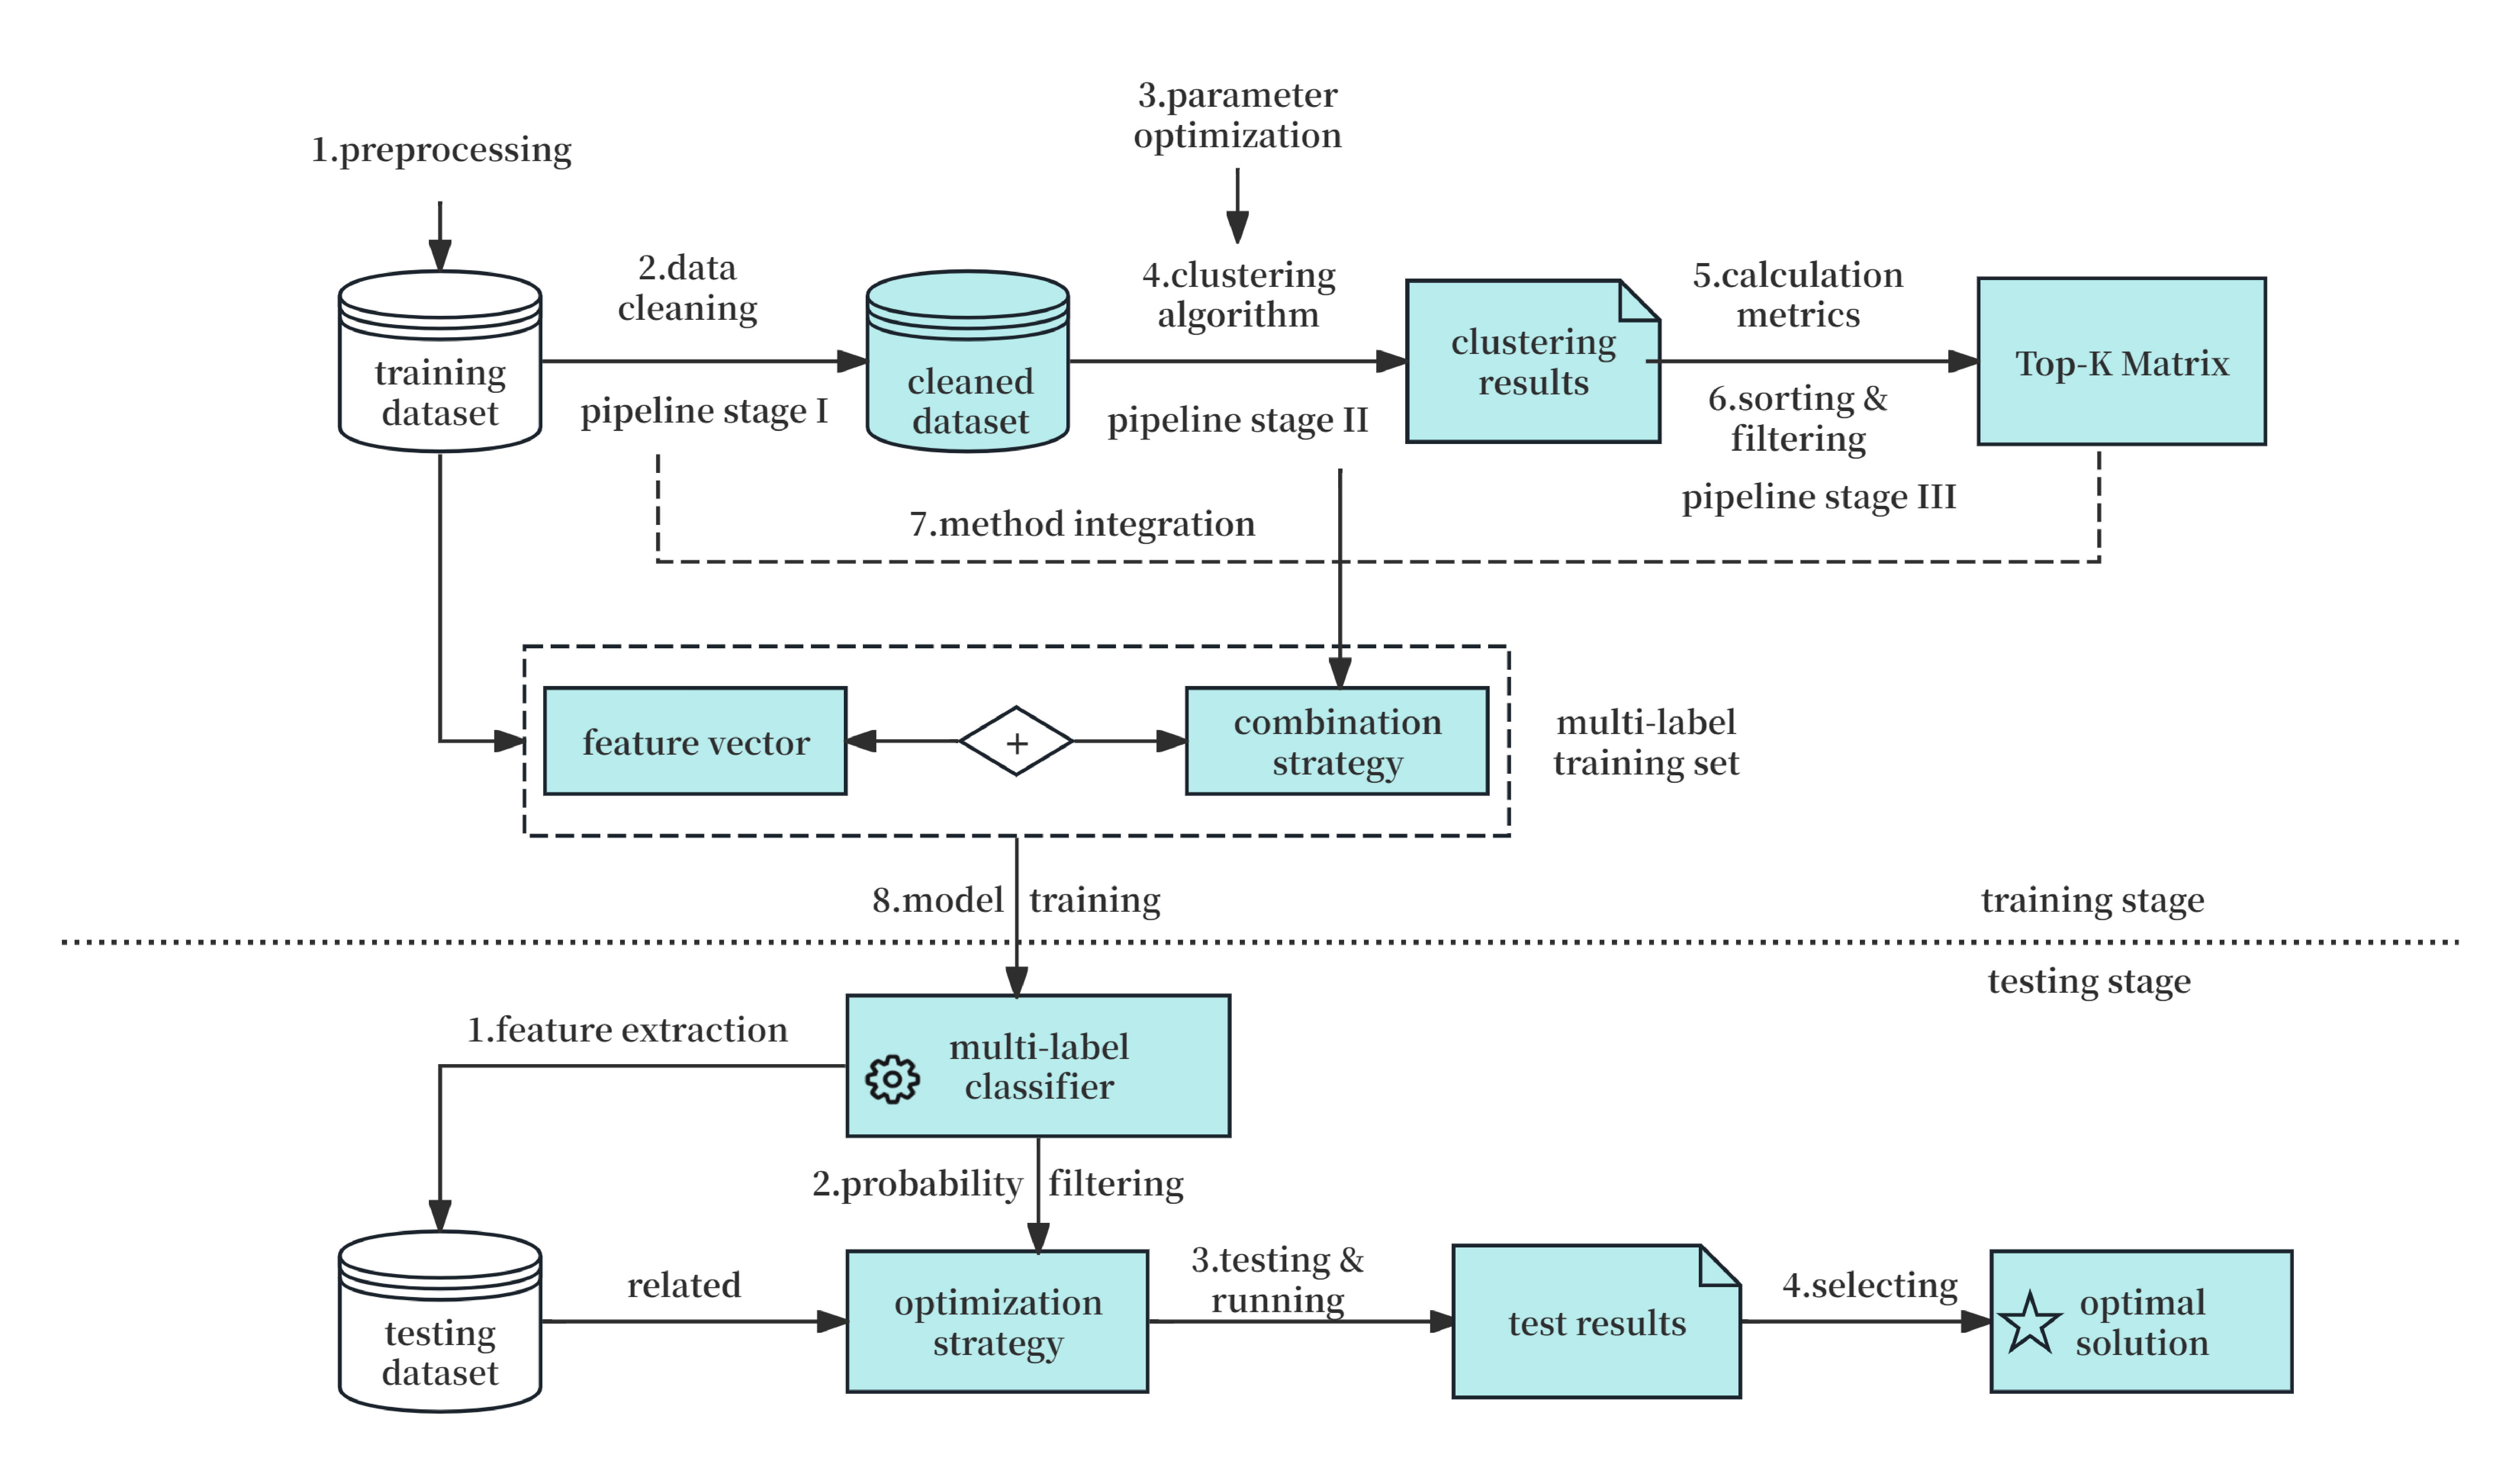
\includegraphics[width=0.9\linewidth]{figures/4graph/autocluster_workflow.pdf}
  \caption{自动化聚类优化流程示意图}
  \label{fig:autocluster-workflow}
\end{figure}

该流程主要包括\textbf{离线知识积累}(训练阶段)和\textbf{在线优化}(测试阶段)两个核心环节:
\begin{enumerate}
    \item \textbf{训练阶段(离线学习)}:基于先验数据集 $D_{\text{train}}$,计算不同数据特征与清洗-聚类策略的匹配程度,并训练多标签分类器 $\mathcal{F}$,从而建立数据特征到优选方案子空间的映射 $G(\mathbf{x}(D))$;同时收集并记录清洗准确度、聚类过程数据,以备深入机理分析。
    \item \textbf{测试阶段(在线优化)}:面对新的数据集 $D_{\text{test}}$,利用训练阶段学习到的映射 $G(\mathbf{x}(D_{\text{test}}))$,快速筛选搜索空间 $\Omega$ 中的候选策略子集 $\Omega'(D_{\text{test}})$,避免全量穷举,从而在较短时间内获取高质量的清洗-聚类方案。若需进一步探讨其内在机制,可通过与离线记录的分布及过程数据比对来解释为何某些组合在新数据上表现突出或失效。
\end{enumerate}

在接下来的小节中,我们将给出训练与测试环节的关键算法伪代码,并展示如何将多标签训练集 $\mathcal{M}$ 与在线推荐结果有机结合。

\subsubsection{训练阶段:离线知识积累}
训练阶段的目标是基于先验数据集 \(D_{\text{train}}\) 生成多标签训练集并学习多标签分类器。算法伪代码如算法~\ref{alg:train-phase} 所示。

\begin{algorithm}[t]
\caption{离线训练阶段:生成训练数据与训练多标签分类器}
\label{alg:train-phase}
\KwIn{
    先验数据集 $D_{\text{train}}=\{D^{(1)},\dots,D^{(N)}\}$;\\
    搜索空间 $\Omega$;\\
    Top-K 大小 $K$。
}
\KwOut{多标签分类器 $\mathcal{F}$}

\SetKwFunction{GenerateTrainingData}{GenerateTrainingData}
\SetKwFunction{TrainClassifier}{TrainClassifier}

$\mathcal{M} \leftarrow \GenerateTrainingData(D_{\text{train}}, \Omega, K)$\;
$\mathcal{F} \leftarrow \TrainClassifier(\mathcal{M})$\;
\KwRet{$\mathcal{F}$}

\bigskip

\SetKwProg{Fn}{Function}{:}{}
\Fn{\GenerateTrainingData{$D_{\text{train}}, \Omega, K$}}{
  $\mathcal{M} \leftarrow \emptyset$\;
  \For{$i \leftarrow 1$ \KwTo $|D_{\text{train}}|$}{
    \ForEach{$\omega \in \Omega$ \textbf{(或采样自 $\Omega$)}}{
      计算 $S(D^{(i)}, \omega)$\;
      记录 EDR/F1 等清洗准确度,以及算法内部过程数据(如质心迭代、核心点等)\;
    }
    选出 Top-K 策略 $\mathbf{M}^{(i)} = \{\omega_1^{(i)}, \dots, \omega_K^{(i)}\}$ 按得分降序\;
    映射为多标签集合 $\mathbf{L}^{(i)} = \{\ell_{\omega_1^{(i)}}, \dots, \ell_{\omega_K^{(i)}}\}$\;
    $\mathcal{M} \leftarrow \mathcal{M} \cup \{(\mathbf{x}(D^{(i)}), \mathbf{L}^{(i)})\}$\;
  }
  \KwRet{$\mathcal{M}$}
}

\Fn{\TrainClassifier{$\mathcal{M}$}}{
  \tcp{可根据具体多标签算法实现}
  训练多标签分类器 $\mathcal{F}$\;
  \KwRet{$\mathcal{F}$}
}
\end{algorithm}

\subsubsection{测试阶段:在线预测与最优方案搜索}
测试阶段在新数据集 \(D_{\text{test}}\) 上应用训练好的分类器,快速锁定优选子空间并搜索最优策略。伪代码如算法~\ref{alg:test-phase} 所示。

\begin{algorithm}[t]
\caption{测试阶段:寻找最优方案 \(\hat{\omega}\)}
\label{alg:test-phase}
\KwIn{
    测试数据集 $D_{\text{test}}$;\\
    多标签分类器 $\mathcal{F}$;\\
    搜索空间 $\Omega$;\\
    保留标签数 $r$。
}
\KwOut{最优方案 $\hat{\omega}$}

计算 $\mathbf{x}(D_{\text{test}})$\;
$\mathbf{L}' \leftarrow \{\}$\;
\ForEach{$\ell \in \mathcal{L}$}{
  $q_{\ell} \leftarrow \text{置信度}(\mathcal{F}, \mathbf{x}(D_{\text{test}}), \ell)$\;
  $\mathbf{L}' \leftarrow \mathbf{L}' \cup \{(\ell, q_{\ell})\}$\;
}
选取置信度最高的 $r$ 个标签 $\mathbf{L}'_{\mathrm{top}}$\;
映射回优选子空间 $\Omega'(D_{\text{test}})$\;
\ForEach{$\omega \in \Omega'(D_{\text{test}})$}{
    计算 $S(D_{\text{test}}, \omega)$ \tcp*{计算综合得分}
}
$\hat{\omega} \leftarrow \arg\max_{\omega \in \Omega'(D_{\text{test}})}S(D_{\text{test}}, \omega)$\;
\KwRet{$\hat{\omega}$}
\end{algorithm}

\subsection{小结}
本节系统介绍了自动化聚类方法的整体框架,从离线阶段的多标签训练与清洗准确度/过程数据记录,到在线阶段通过优选子空间快速搜索最优策略。在此基础上,我们不仅能在\textbf{大规模搜索空间}中高效获得近优清洗-聚类组合,还能借助\textbf{记录下的清洗精度与算法过程}信息,对清洗操作对聚类结果的影响机理进行更深入的剖析。下一章我们将结合具体实验展示该方法在多场景下的适用性与可解释性。


%---------------------------------
% 第五章:实验与结果分析
%---------------------------------

\section{宏观实验与现象归纳}
\label{sec:chapter5}

本章围绕第~\ref{sec:problem-and-model} 节所提出的问题和模型定义(特别是第~\ref{subsec:problem-statement} 节)展开实验与结果分析,通过对多种数据集和聚类算法的验证,定量评估“数据清洗与聚类协同优化”方案的有效性和适用性。
\vspace{-0.5em}
%--------------------------------------------------
\subsection{\textcolor[rgb]{0.00,0.07,1.00}{实验设置}}\label{sec:exp_setting}
%--------------------------------------------------

\textcolor[rgb]{0.00,0.07,1.00}{本章实验紧扣第~\ref{sec:problem-and-model} 节提出的“多错误特征向量”理论。
理论模型允许单元格同时出现多种脏污,但在实验阶段我们做出如下\textbf{可控退化}:}

\begin{enumerate}[label=\arabic*), leftmargin=2em]
\item \textcolor[rgb]{0.00,0.07,1.00}{仅保留两种最基本的错误类型:\textbf{缺失值 (Missing)} 与
      \textbf{异常值 (Anomaly)};}  

\item \textcolor[rgb]{0.00,0.07,1.00}{同一单元格至多含一种错误,
      因此在实验中
      \[
          r_{\text{tot}}(D)\;=\;
          r_{\text{miss}}(D)+r_{\text{anom}}(D).
      \]}
\vspace{-2em}
\item \textcolor[rgb]{0.00,0.07,1.00}{\textbf{异常值难以在真实数据中精确计数},
      故我们将“注入错误比例”当作
      $r_{\text{anom}}(D)$;  
      缺失值则在运行时精确统计,
      得到 $r_{\text{miss}}(D)$。}  
\end{enumerate}

\textcolor[rgb]{0.00,0.07,1.00}{于是本章用于多标签学习及 AutoML 的实验特征向量为  
\[
  \mathbf{x}_{\text{exp}}(D)=
  \bigl(
      r_{\text{tot}},\,
      r_{\text{miss}},\,
      r_{\text{anom}},\,
      m,\,n
  \bigr),\qquad
  r_{\text{tot}}=r_{\text{miss}}+r_{\text{anom}}.
\]}

\vspace{-3em}

%--------------------------------------------------
\subsubsection{数据集准备}\label{sec:dataset_prep}
%--------------------------------------------------

\textcolor[rgb]{0.00,0.07,1.00}{本研究选用 4 个在数据清洗文献中被广泛引用的公开数据集
\emph{beers}, \emph{flights}, \emph{hospital}, \emph{rayyan}。
对于每个数据集的\textbf{干净副本},在除主键列外的所有单元格独立注入
\((\text{AnomalyRate},\text{MissingRate})\in\{0,5,10,15\}\%\times\{0,5,10,15\}\%\),
共产生 \(4\times4-1=15\) 份含错文件(排除 \(0\%–0\%\) 组合)。
表 \ref{tab:dataset_overview} 给出了四个数据集的规模 \((n,m)\),
理论注入搜索网格(两类错误的参数均为 0–15\%),
以及 15 份带错文件\textbf{观测}总错误率
\(r_{\text{tot}}=r_{\text{anom}}+r_{\text{miss}}\) 的最小–最大区间。}

\begin{table}[htbp]
  \centering
  \setlength{\tabcolsep}{5pt}
  %\begin{adjustbox}{width=\linewidth}
  \begin{tabular}{lcccc}
    \toprule
    \textbf{数据集} & $n$ & $m$ & \textbf{理论注入(\%)} & $r_{\text{tot}}^{\min}$--$r_{\text{tot}}^{\max}$ (\%)\\
    \midrule
    beers    & 2\,410 & 11 & 0--15 (Anom./Miss.) & 9.23--33.10 \\
    flights  & 2\,376 & 7  & 0--15 (Anom./Miss.) & 4.99--29.99 \\
    hospital & 1\,000 & 20 & 0--15 (Anom./Miss.) & 5.00--30.00 \\
    rayyan   & 1\,000 & 12 & 0--15 (Anom./Miss.) & 18.74--39.85 \\
    \bottomrule
  \end{tabular}
  %\end{adjustbox}
  \caption{四个数据集的规模、理论注入区间与观测总错误率范围}
  \label{tab:dataset_overview}
\end{table}

\noindent
\textcolor[rgb]{0.00,0.07,1.00}{表中所有任务均满足 \(r_{\text{tot}} = r_{\text{anom}} + r_{\text{miss}}\)
后续的多标签学习与 AutoML 管线直接采用
\[
  \mathbf{x}_{\text{exp}}
  = \bigl(r_{\text{tot}},\,r_{\text{miss}},\,r_{\text{anom}},\,m,\,n\bigr)
\]
作为数据特征输入。}


\subsubsection{算法准备}
\label{sec:algo_prep}

本研究关注两方面算法:
(1) \textbf{数据清洗策略};(2) \textbf{聚类算法及对应参数}。

\paragraph{数据清洗策略}   
\textcolor[rgb]{0.00,0.07,1.00}{为便于后续实验复现与比较,表 \ref{tab:clean_algo_overview} 初步汇总了本研究选取的 9 种清洗方法的关键信息。读者可据此快速了解各算法在本章实验中的角色与设置;其具体原理及对聚类过程的影响分析将在第 6 章展开。}

\begin{table}[htbp]
\centering
\small
\renewcommand{\arraystretch}{1.15}
\setlength{\tabcolsep}{4pt}
%\begin{adjustbox}{width=\linewidth}
\begin{tabular}{@{}lcccc@{}}
\toprule
\textbf{算法} & \textbf{针对错误类型} & \textbf{必需配置} &
\textbf{模型范式} & \textbf{清洗目标} \\
\midrule
Mode Impute & MV, FI & — &
统计填补 & \textit{Repair} \\

Raha-Baran & MV, FI, Rule viol. & 无显式约束 &
端到端 ML & \textit{Detect + Repair} \\

HoloClean & MV, FI, Dup, Rule viol. &
FD/CF + 外部知识 &
概率图模型 & \textit{Detect + Repair} \\

BigDansing & Schema viol., Typos &
检测规则 & 规则驱动 & \textit{Detect} \\

BoostClean & Label/Attr Noise &
下游模型 (监督) &
Boosting Ensemble & Task–Aware Repair \\

Horizon & MV, Outlier &
时序窗口宽度 &
时序/统计混合 & \textit{Repair} \\

Scared & MV, FI, Outlier &
半监督标注预算 &
主动学习模型 & \textit{Detect + Repair} \\

Unified & MV, Rule viol., Dup &
统一约束文件 &
多策略融合 & \textit{Detect + Repair} \\

GroundTruth & — & — &
理想基线 & \textit{Upper Bound} \\
\bottomrule
\multicolumn{5}{l}{\footnotesize
MV: Missing Value;FI: Format Inconsistency;Dup: Duplicate;Rule~viol.: 约束违规。}
\end{tabular}
%\end{adjustbox}
\caption{实验用 9 种数据清洗方法总览(本章仅作简述,机理详见第 6 章)}
\label{tab:clean_algo_overview}
\end{table}

\vspace{-1em}

\paragraph{聚类算法}
\textcolor[rgb]{0.0,0.07,1.0}{%
表 \ref{tab:algo_overview_ch5} 简要列出了本章所使用的 6 类定制化聚类脚本在初始化、超参搜索、过程追踪及复杂度方面相较于 \texttt{scikit-learn} 标准实现的主要调整。其设计动机在于为第 5 章实验提供统一且可追踪的运行记录;更深入的原理剖析与过程指标解读将在第 6 章展开。}

\begin{table}[t]
\centering
\small
\setlength{\tabcolsep}{4pt}
\renewcommand{\arraystretch}{1.05}
%\begin{adjustbox}{width=\linewidth}
\begin{tabular}{@{}lccccc@{}}
\toprule
\textbf{算法名称} &
\textbf{初始化策略} &
\textbf{参数调优} &
\makecell[c]{\textbf{过程指标}\\(方向)} &
\makecell[c]{\textbf{复杂度}\\变化} \\ 
\midrule
K-Means\textsubscript{base} &
k-means++ &
Optuna($k$) &
$\Delta n_{\text{iter}}\!\downarrow$, AUC$_\Delta\!\downarrow$ &
$\uparrow$ $\mathcal{O}(nkT)$ \\

K-Means\textsubscript{PPS}\cite{10.5555/3016100.3016103} &
K-MC$^{2}$ 采样 &
Optuna($k$) &
同上 &
$\downarrow$ $\mathcal{O}(n)$ init \\

K-Means\textsubscript{NF}\cite{10.1109/TKDE.2022.3155450} &
随机标签$\!\to\!F$ &
Optuna($k$) &
同上 &
$\uparrow$ (Gram) \\

GMM-EM (tracking) &
k-means++ &
Optuna+Kneedle($k$) &
$\Delta n_{\text{iter}}\!\downarrow$, AUC$_{\text{LL}}\!\downarrow$ &
$\uparrow$ (warm start 循环) \\

DBSCAN (noise-aware) &
— &
Optuna($\varepsilon$, minPts) &
$\Delta n_\text{core}\!\uparrow$, $\Delta\rho_\text{noise}\!\downarrow$ &
$\approx\mathcal{O}(n\log n)$ \\

HC (merge-tree) &
— &
Optuna($k$)+linkage+metric &
$\Delta n_\text{merge}\!\downarrow$, $\Delta h_{\max}\!\downarrow$ &
$\mathcal{O}(n^{2})$ \\
\bottomrule
\end{tabular}
%\end{adjustbox}

\caption{6种定制化聚类脚本的初始化策略、调参方式、过程指标及复杂度概览}
\label{tab:algo_overview_ch5}
\end{table}

%--------------------------------------------------
\subsection{实验流程}
\label{sec:exp_flow}
%--------------------------------------------------

本节给出大规模统计实验的标准流水线(图~\ref{fig:exp_flow}),覆盖本章后续所有结果所需的输入与输出。整个链条将做数据与指标采集,但并不在此阶段训练或调用 AutoML;步骤 4 产生的中间文件将在第~\ref{sec:chapter6} 章用作 AutoML 特征与标签。

\begin{figure}[htbp]
  \centering
  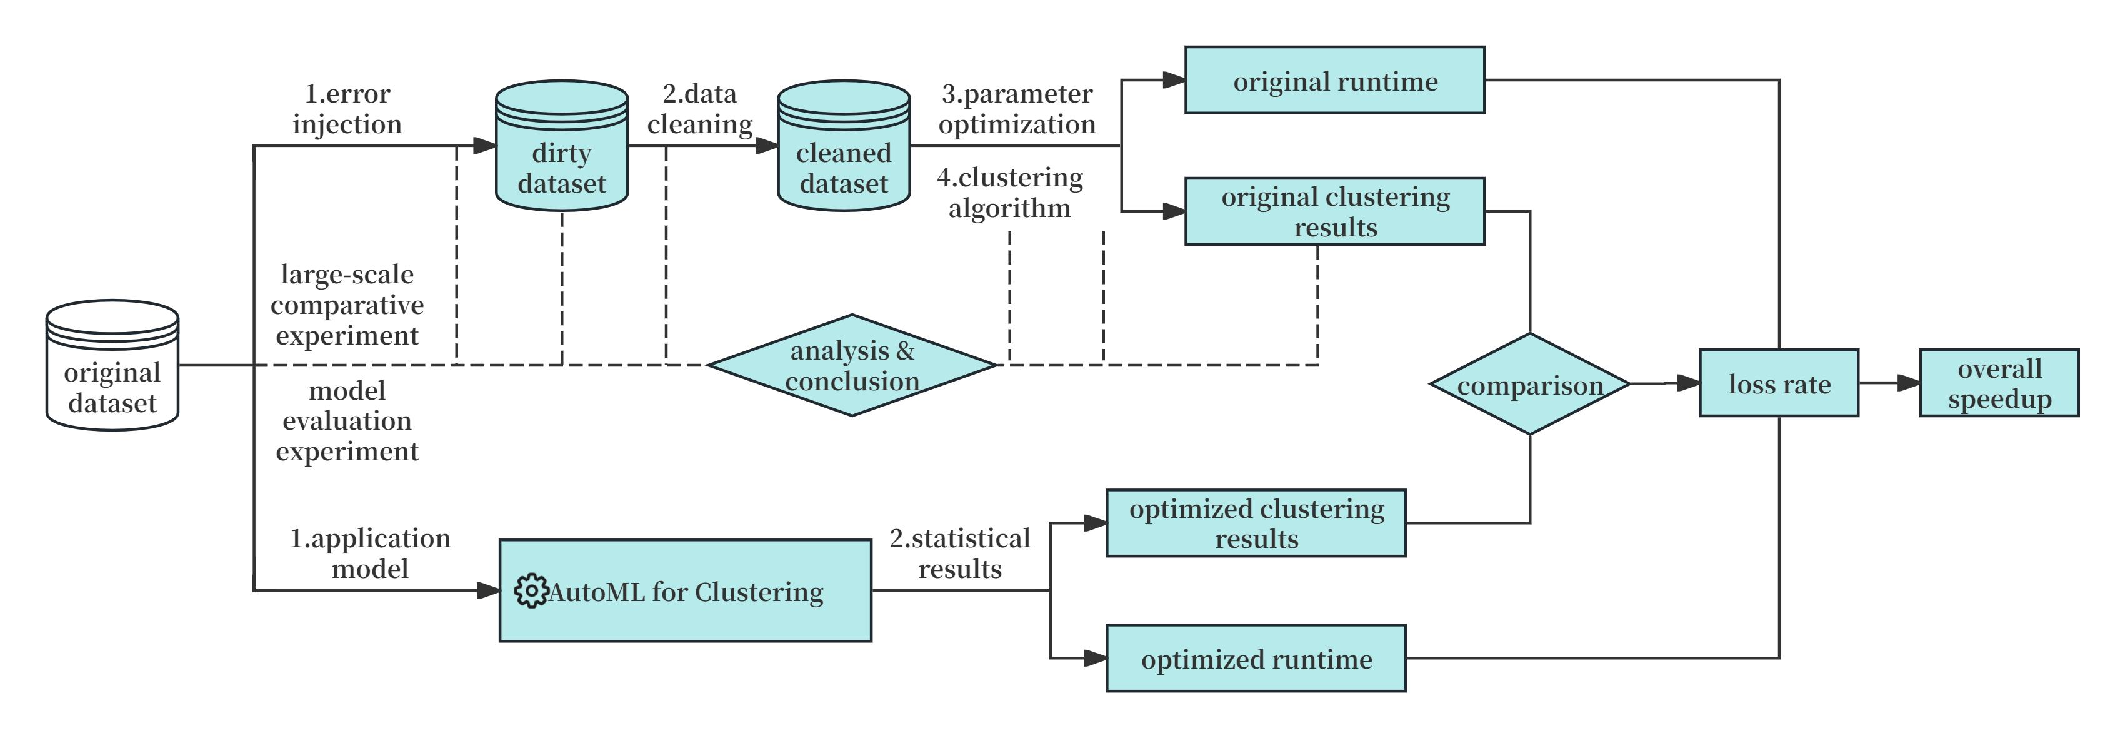
\includegraphics[width=0.95\linewidth]{figures/4graph/exp_workflow.pdf}
  \caption{本章批量实验的四阶段流水线}
  \label{fig:exp_flow}
\end{figure}

\begin{enumerate}[label=\textbf{Step\,\arabic*.}, itemindent=4em, leftmargin=0pt]

\item \textbf{可控错误注入 \& 特征统计}  \\
\textcolor[rgb]{0.00,0.07,1.00}{对每个干净数据集依照 \((\text{AnomalyRate},\text{MissingRate}) \in \{0,5,10,15\}\,\%\) 的网格注入错误,生成 15 份含错版本。运行时即时统计 \(\{r_{\text{tot}},\,r_{\text{miss}},\,r_{\text{anom}},\,m,\,n\}\),形成特征向量 \(\mathbf{x}_{\text{exp}}(D)\)。}

\item \textbf{清洗 $\rightarrow$ 聚类批处理}  \\
\textcolor[rgb]{0.00,0.07,1.00}{对每个含错文件分别执行 9种清洗算法(表 \ref{tab:clean_algo_overview})并采集结果;随后用 6 种定制化聚类脚本(表 \ref{tab:algo_overview_ch5})进行聚类与超参搜索,同时记录过程指标(迭代步数、质心位移、核心点等)。}

\item \textbf{指标计算与分档}  \\
\textcolor[rgb]{0.00,0.07,1.00}{对聚类输出计算 Silhouette、Davies–Bouldin 与 Combined Score,并把全部原始指标汇总为三类实验:  
(i) 得分评估 —— 跨多种清洗-聚类组合的结果求均值/方差;  
(ii) 错误率梯度 —— 按 \(r_{\text{tot}}\) 分档绘制曲线;  
(iii) 错误类型对比 —— 固定 \(r_{\text{tot}}\) 比较 \(r_{\text{miss}}\) 与 \(r_{\text{anom}}\) 的影响。}

\item \textbf{结果持久化}  \\
\textcolor[rgb]{0.00,0.07,1.00}{将每个错误数据集的清洗标签、聚类历史、超参数与评估指标统一记录,同时导出 \(\bigl(\mathbf{x}_{\text{exp}},\,\Omega^{\star},\,S^{\star}\bigr)\) 三元组作为 AutoML 训练样本。}

\end{enumerate}

\noindent
完成上述 4 步后,我们即将在第~\ref{sec:score_eval_exp} 节到
第~\ref{sec:error_sense_exp} 节
分别开展“得分评估”与“错误敏感性”三组实验,
初步回答第~\ref{subsec:problem-statement} 节中提出的问题挑战。

%--------------------------------------------------
\subsection{\textcolor[rgb]{0.00,0.07,1.00}{实验结果与分析}}
\label{sec:exp_results}
%--------------------------------------------------

在完成第~\ref{sec:exp_flow} 节所述四阶段实验流水线后,
我们对全部 \(\,60\) 份错误数据集
\(\times\) 9 种清洗 \(\times\) 6 种聚类
共 \(60\times9\times6=3\,240\) 组运行结果进行统计分析。
本节按照由粗略到细致、由全局到局部的思路拆分为三项对照实验:

\begin{enumerate}[leftmargin=2.5em]
  \item \textbf{得分评估实验}(\S\ref{sec:score_eval_exp})  
        —— 横向比较 9\(\times\)6 种“清洗+聚类”组合在
        平均分、方差等维度的全局表现;
  \item \textbf{错误敏感性实验}(\S\ref{sec:error_sense_exp})  
        —— 将 \(r_{\text{tot}}\) 以 5 \% 为步长分档,  
        同时在固定 \(r_{\text{tot}}\) 的前提下改变
        \(\bigl(r_{\text{miss}},r_{\text{anom}}\bigr)\) 二元比例,  
        统一考察错误率递增与错误类型差异对聚类指标的综合影响。
\end{enumerate}

下面首先给出 5.3.1 的详细结果。

%--------------------------------------------------
%--------------------------------------------------
\subsubsection{\textcolor[rgb]{0.00,0.07,1.00}{得分评估实验}}
\label{sec:score_eval_exp}
%--------------------------------------------------

\paragraph{实验目的与统计指标}
本子实验从“绝对效果 / 相对效果 / 方法稳定性”三个维度,
评估每一个 \(\langle\!\text{清洗},\text{聚类}\!\rangle\) 固定组合在
60 份含错数据集中的整体表现。
记 \(S=\text{Combined Score}\),
\(S_{\mathrm{GT}}\) 为同数据集 \textit{Ground-Truth} 清洗下的得分,
则采集三项统计量
\[
  \Bigl(
    \overline{S},\;
    \overline{S}_{\%\mathrm{GT}},\;
    \sigma^{2}_{S}
  \Bigr), \qquad
  \overline{S}_{\%\mathrm{GT}}
    =\frac{1}{N}\sum_{i=1}^{N}\frac{S_i}{S_{i,\mathrm{GT}}}\times100\%.
\]

\begin{itemize}[leftmargin=1.9em]
  \item \(\overline{S}\):绝对平均分;直接对 \(S\) 取算术均值。
  \item \(\overline{S}_{\%\mathrm{GT}}\):相对平均分;先对每条记录做
        “除以 \(S_{\mathrm{GT}}\) 后乘 \(100\%\)” 的归一化,再取均值,
        用于跨数据集的横向比较。
  \item \(\sigma^{2}_{S}\):得分方差;衡量组合在不同数据-错误场景下
        的波动风险——方差越大,出现“爆分 / 翻车”的概率越高。
\end{itemize}

\vspace{0.3em}
%--------------------------------------------------
\paragraph{结果可视化}
针对每个数据集(beers、flights、hospital、rayyan)各生成三幅图:

\begin{enumerate}[label=\arabic*) ,leftmargin=1.2em]
  \item \emph{相对平均分热力图}\\
        \(9\times6\) 单元;颜色 = \(\overline{S}_{\%\mathrm{GT}}\),
        单元格右下角小灰字 = \(\sigma^{2}_{S}\)。
        直观看出“最深蓝”块即全局最佳组合。
  \item \emph{均值–方差散点图}\\
        X 轴 = \(\overline{S}_{\%\mathrm{GT}}\),
        Y 轴 = \(\sigma^{2}_{S}\)。
        点颜色代表清洗方法,点形状代表聚类算法,
        在同一平面呈现“收益–风险”权衡。
  \item \emph{Top-10 带误差条形图}\\
        选该数据集上 \(\overline{S}_{\%\mathrm{GT}}\) 最高的 10 个组合:
        横轴 = \(\overline{S}_{\%\mathrm{GT}}\),
        误差条 = \(\pm\sqrt{\sigma^{2}_{S}}\),并用虚线标出 \(100\%\) 基准。
\end{enumerate}

\begin{figure}[htbp]
  \centering
  \footnotesize
  \setlength{\abovecaptionskip}{4pt}
  \setlength{\belowcaptionskip}{0pt}

  % ---------- beers ----------
  \begin{subfigure}{0.33\linewidth}
    \centering
    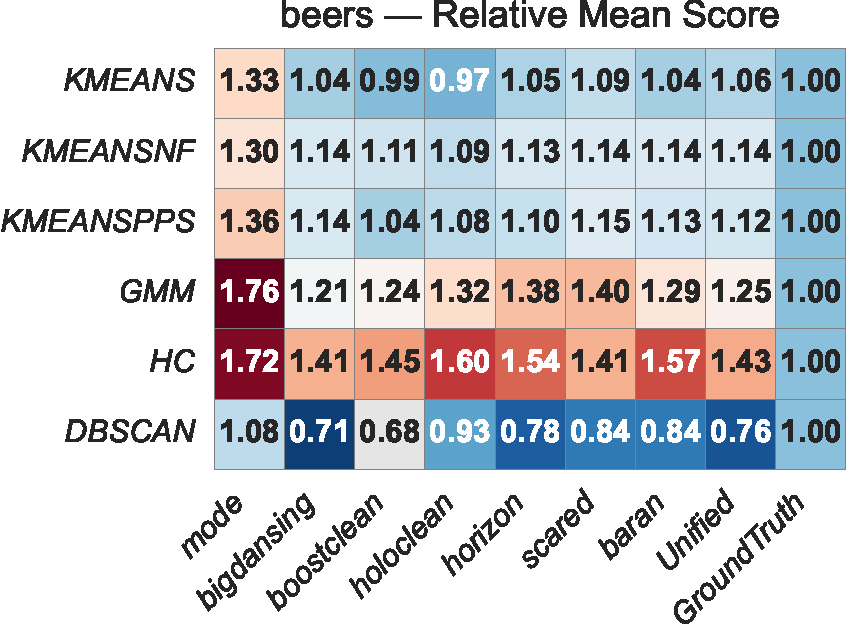
\includegraphics[width=\linewidth]{figures/5.3.1graph/heatmap_rel_beers.pdf}
    \caption{Heat-map · beers}
  \end{subfigure}\hfill
  \begin{subfigure}{0.32\linewidth}
    \centering
    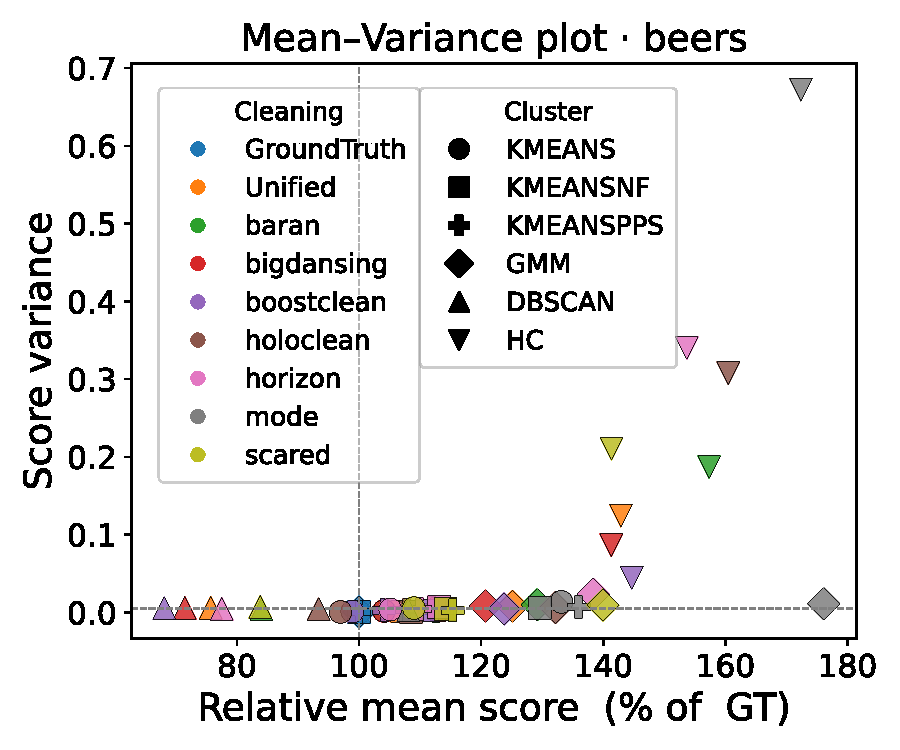
\includegraphics[width=\linewidth]{figures/5.3.1graph/mean_var_scatter_beers.pdf}
    \caption{Mean–Var · beers}
  \end{subfigure}\hfill
  \begin{subfigure}{0.34\linewidth}
    \centering
    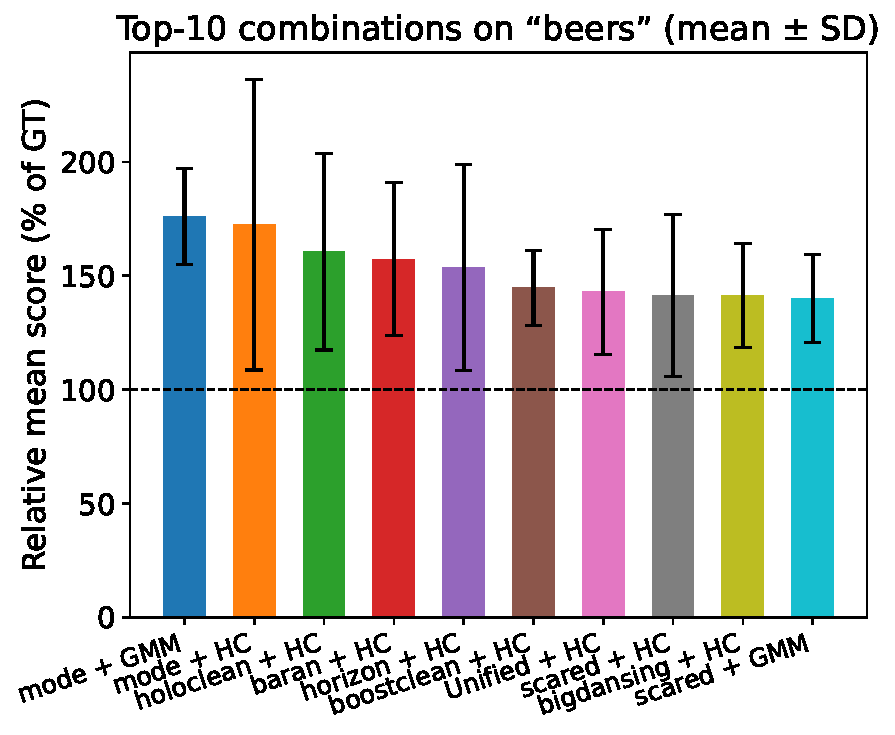
\includegraphics[width=\linewidth]{figures/5.3.1graph/top10_bar_error_beers.pdf}
    \caption{Top-10 · beers}
  \end{subfigure}

  \vspace{0.6em}
  % ---------- flights ----------
  \begin{subfigure}{0.33\linewidth}
    \centering
    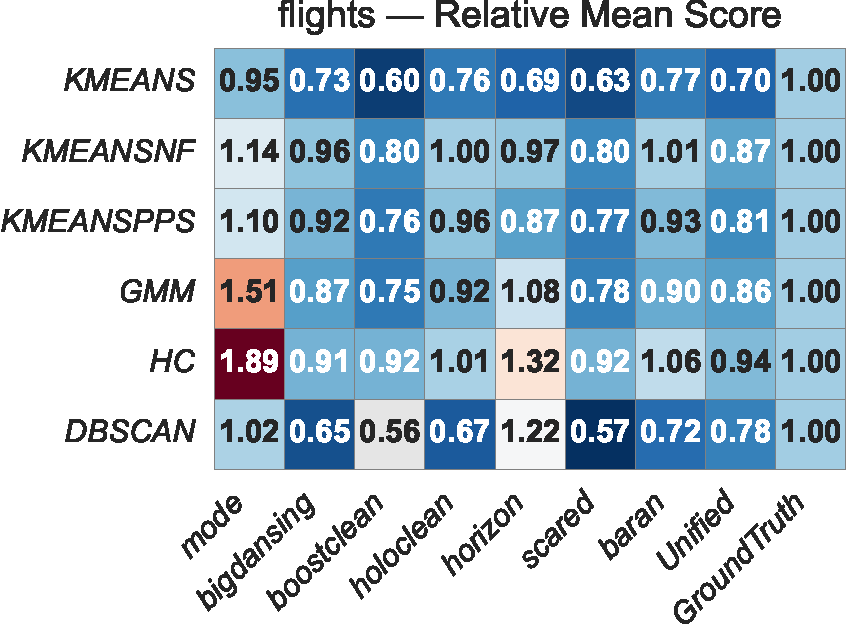
\includegraphics[width=\linewidth]{figures/5.3.1graph/heatmap_rel_flights.pdf}
    \caption{Heat-map · flights}
  \end{subfigure}\hfill
  \begin{subfigure}{0.32\linewidth}
    \centering
    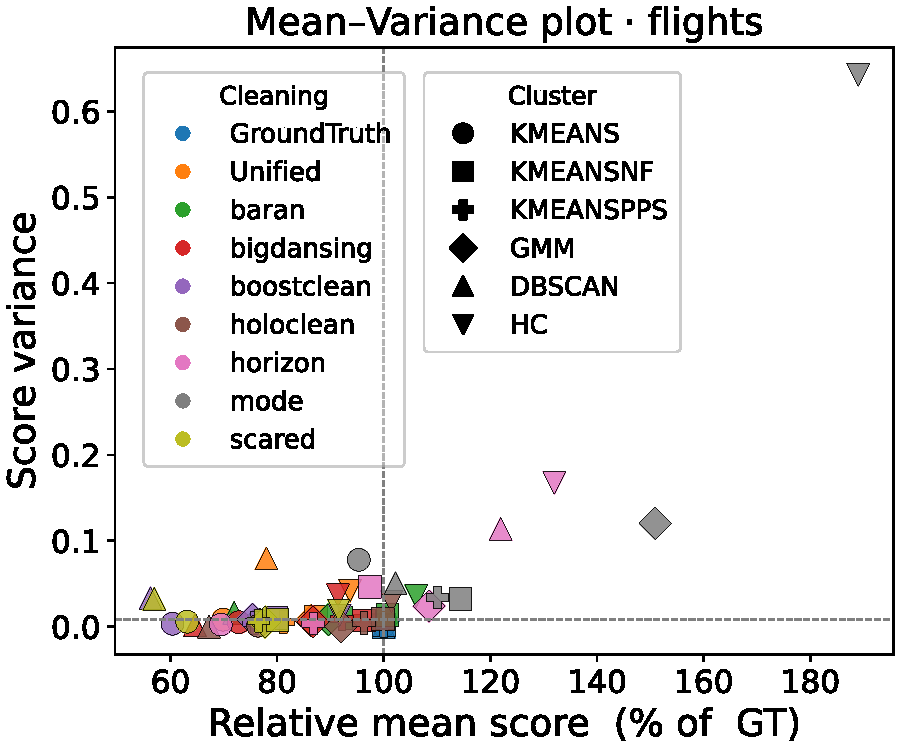
\includegraphics[width=\linewidth]{figures/5.3.1graph/mean_var_scatter_flights.pdf}
    \caption{Mean–Var · flights}
  \end{subfigure}\hfill
  \begin{subfigure}{0.34\linewidth}
    \centering
    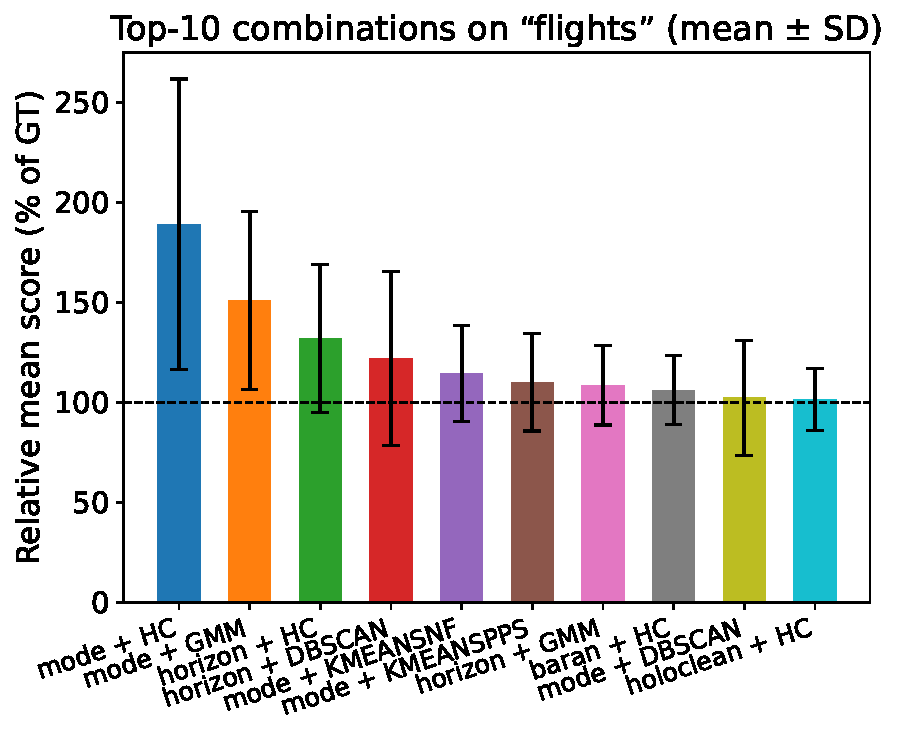
\includegraphics[width=\linewidth]{figures/5.3.1graph/top10_bar_error_flights.pdf}
    \caption{Top-10 · flights}
  \end{subfigure}

  \vspace{0.6em}
  % ---------- hospital ----------
  \begin{subfigure}{0.33\linewidth}
    \centering
    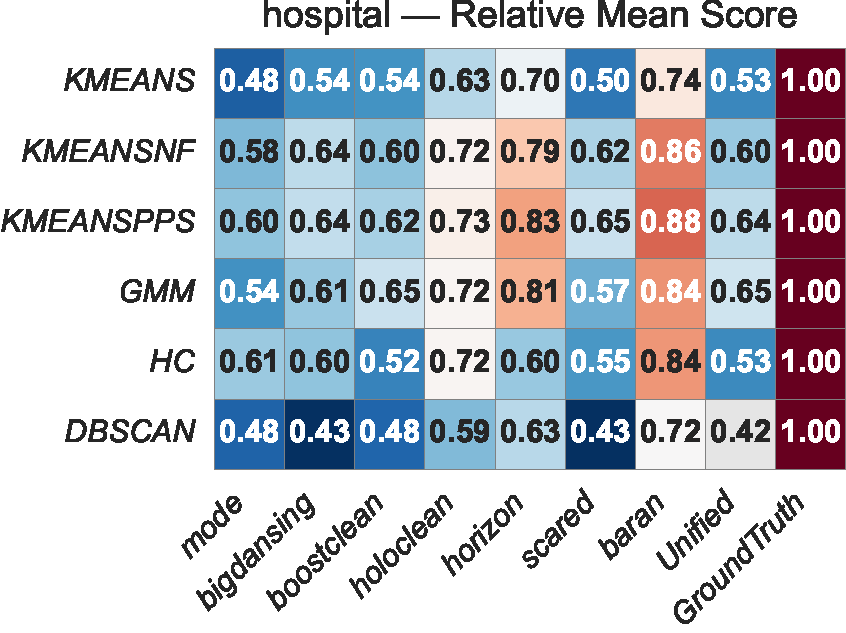
\includegraphics[width=\linewidth]{figures/5.3.1graph/heatmap_rel_hospital.pdf}
    \caption{Heat-map · hospital}
  \end{subfigure}\hfill
  \begin{subfigure}{0.32\linewidth}
    \centering
    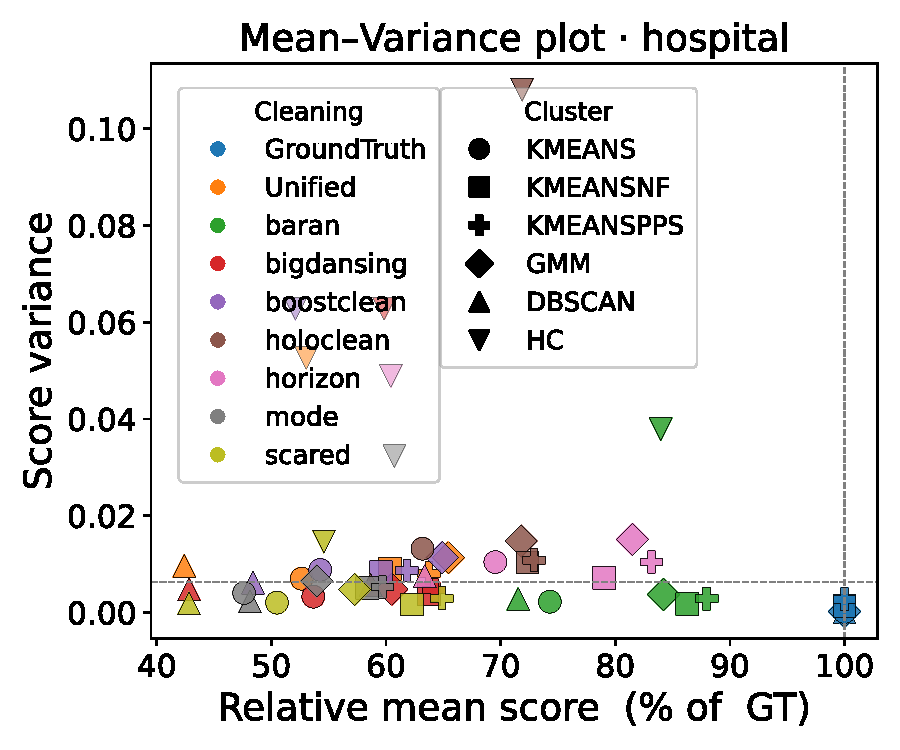
\includegraphics[width=\linewidth]{figures/5.3.1graph/mean_var_scatter_hospital.pdf}
    \caption{Mean–Var · hospital}
  \end{subfigure}\hfill
  \begin{subfigure}{0.34\linewidth}
    \centering
    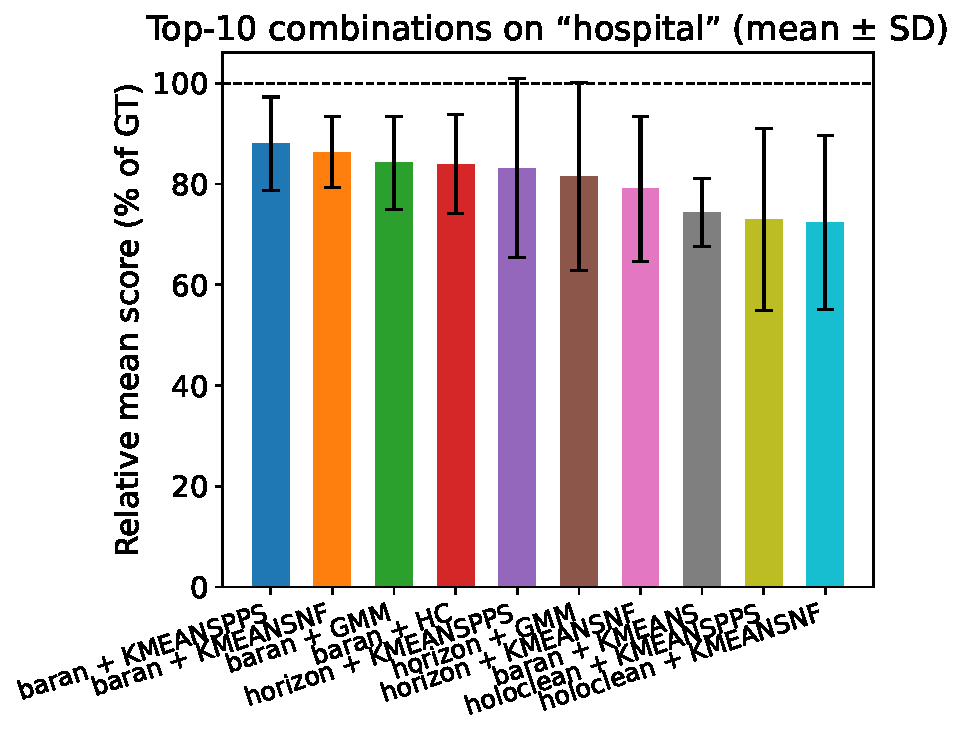
\includegraphics[width=\linewidth]{figures/5.3.1graph/top10_bar_error_hospital.pdf}
    \caption{Top-10 · hospital}
  \end{subfigure}

  \vspace{0.6em}
  % ---------- rayyan ----------
  \begin{subfigure}{0.33\linewidth}
    \centering
    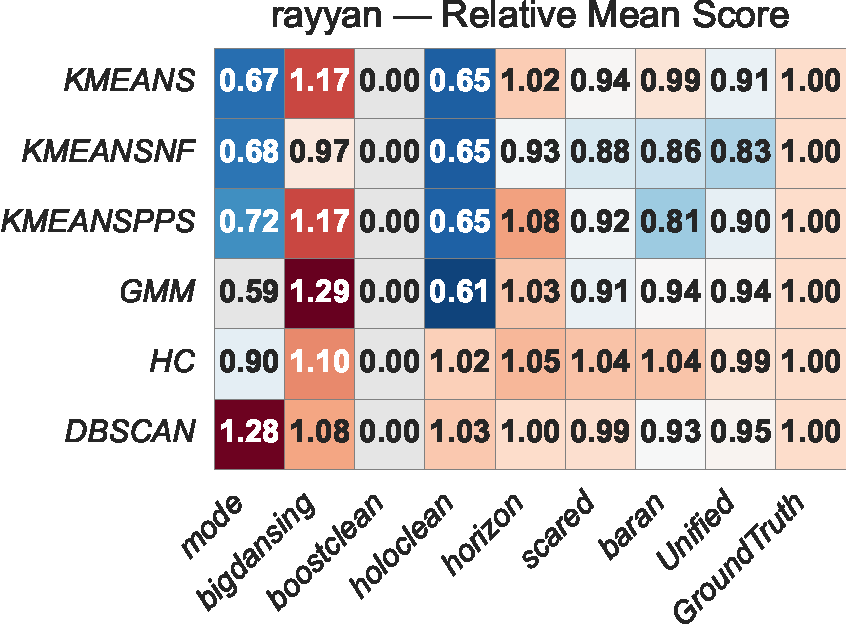
\includegraphics[width=\linewidth]{figures/5.3.1graph/heatmap_rel_rayyan.pdf}
    \caption{Heat-map · rayyan}
  \end{subfigure}\hfill
  \begin{subfigure}{0.32\linewidth}
    \centering
    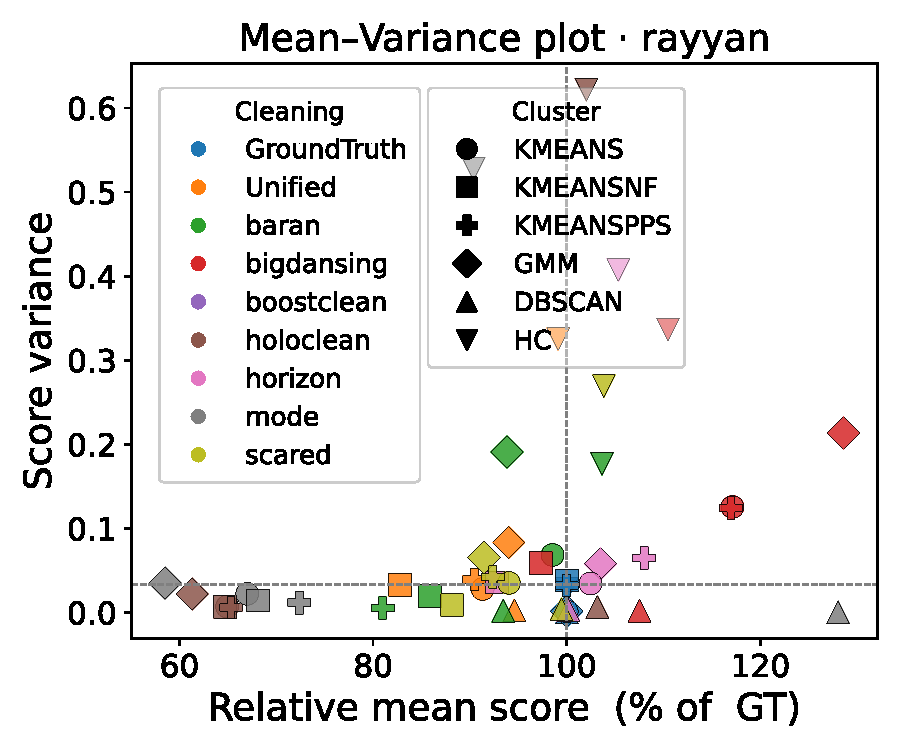
\includegraphics[width=\linewidth]{figures/5.3.1graph/mean_var_scatter_rayyan.pdf}
    \caption{Mean–Var · rayyan}
  \end{subfigure}\hfill
  \begin{subfigure}{0.34\linewidth}
    \centering
    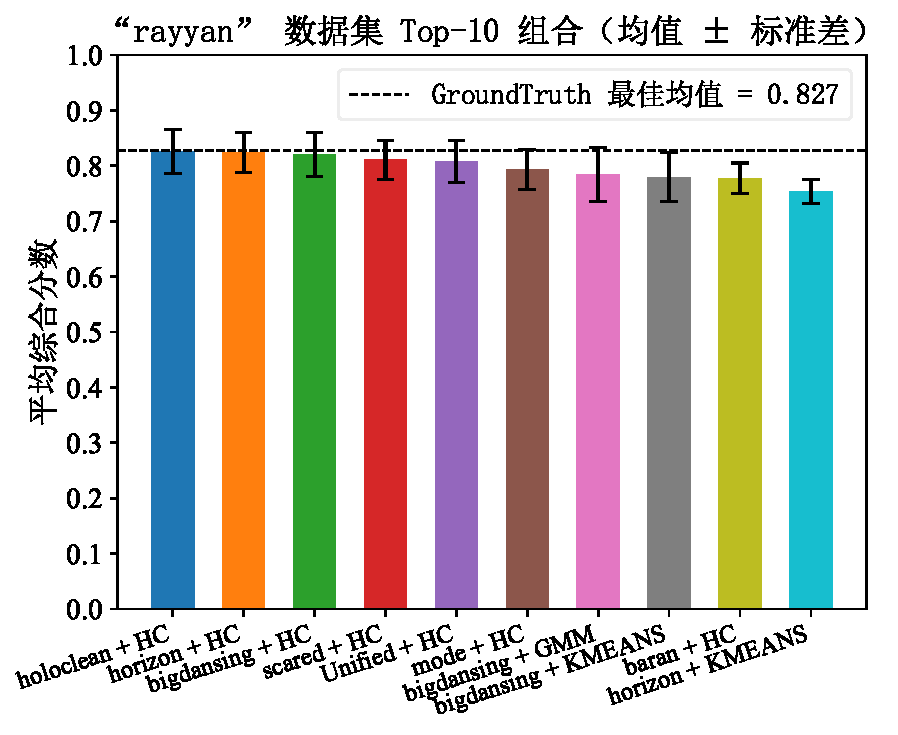
\includegraphics[width=\linewidth]{figures/5.3.1graph/top10_bar_error_rayyan.pdf}
    \caption{Top-10 · rayyan}
  \end{subfigure}

  \caption{三种视角的得分评估结果(每行对应一个数据集)。%
           颜色越深蓝表示 \(\overline{S}_{\%\mathrm{GT}}\) 越高;%
           散点越靠右/越低表示高收益且低风险;%
           条形误差条体现平均收益的置信区间。
           }
  \label{fig:score_eval_all}
\end{figure}

%--------------------------------------------------
\paragraph{结果分析}
\label{sec:score_eval_exp_analysis}
%--------------------------------------------------

图 \ref{fig:score_eval_all} 汇聚了四个数据集在
54 种\(\langle\!\text{清洗},\text{聚类}\!\rangle\) 组合上的
\emph{相对均值热力图}[(a)(d)(g)(j)],
\emph{均值–方差散点}[(b)(e)(h)(k)]
以及 \emph{Top-10 带误差条形图}[(c)(f)(i)(l)]。
综合三种视角可归纳出如下共性与差异。

\begin{enumerate}[label=\textbf{\arabic*.},leftmargin=2.6em]

%--------------------------------------------------------
\item \textbf{多场景最突出的两种组合方案:\texttt{mode+HC} 与 \texttt{GroundTruth+HC}.}\\
在四组 Top-10 图中,
共有 \num{7} 组组合在全部数据集均进入前10名。
其中 \texttt{mode+HC} 与 \texttt{GroundTruth+HC}
分别出现 \num{17} 次与 \num{13} 次第1名,
显著高于其它高频轨迹。Friedman 检验
\(\chi^{2}=\num{1671.4},\,p<2.2\times10^{-16}\)  
\((N=\num{60},\,k=\num{48})\) 与 Kendall 一致系数
\(W=\num{0.593}\) 共同表明整体排序高度一致;
最优与次优组合的平均秩差仅
\(\Delta r=\num{0.1}\),远小于临界差
\(\mathrm{CD}=\num{14.36}\)。两者在 \(\alpha=0.05\) 水平统计上不可区分;
因此最优方案须同时参考频次与稳健性等指标。

%--------------------------------------------------------
\item \textbf{层次聚类增益依赖于 “类间梯度不被压缩”。}\\
在热力图中,
对于\(|\Delta\text{DBI}|<\num{0.40}\) 且
\(\Delta\text{Sil}\) 与 \(\Delta\text{DBI}\) 同号的单元,
\texttt{HC} 行均呈深蓝色;
对应增益-基线斜率
\(\partial G/\partial\text{Sil}=\num{1.32}\),
仅为 K-Means 的 \num{0.54} 倍。
一旦出现 “非同向变化”的情形
(例如 \emph{flights} 中 \(\Delta\text{Sil}>0\),
 \(\Delta\text{DBI}<0\) 的单元格),
HC 在条形图中的名次即跌出前三。
因此 HC 优势取决于层次梯度是否完整保留,
过度清洗或指标冲突均可能抵消此优势。

%--------------------------------------------------------
\item \textbf{文本占优的数据集中出现“众数-密度”方法最优的例外情形。}\\
在最后一行热力图(对应\emph{rayyan} 数据集)中,
\texttt{mode+DBSCAN} 单元显示
\(\overline{S}_{\%\mathrm{GT}}=\num{1.28}\),
而同种方法在 \emph{hospital} 数据集上仅为 \num{0.48}。
这表明高语义冗余文本在向量空间形成致密区域,
DBSCAN 方法会因此规避 HC 的簇碎片化问题,因此可在文本向量为主的数据集中把 DBSCAN 方法放入首选候选而非默认 HC,
并同时扩大参数 \(\varepsilon\) 的搜索上界。

%--------------------------------------------------------
\item \textbf{“理想清洗”方法从总体得分的角度弱于 \texttt{mode}方法。}\\
\texttt{GroundTruth}+HC 的平均
\(\overline{S}_{\%\mathrm{GT}}\) 比
\texttt{mode+HC} 低 \num{0.28},
且差值的 \SI{95}{\percent} 置信区间
\([0.02,\,0.55]\) 不含0。
在第三列的条形图中,\texttt{GroundTruth}+HC
常排第 \numrange{3}{5} 位,
再次量化 “过度修复削弱类间梯度” 的副作用,
证明了F1 得分最高的清洗策略并不总是聚类得分上限。
\end{enumerate}

%--------------------------------------------------
\subsubsection{\textcolor[rgb]{0.00,0.07,1.00}{错误敏感性实验}}
\label{sec:error_sense_exp}
%--------------------------------------------------

\paragraph{实验目的与统计指标}
本实验从两条互补维度定量评估噪声对综合得分 \(S\) 的影响:
\begin{itemize}[leftmargin=1.9em]
  \item \textbf{总错误率梯度}\;(\texttt{error\_rate}) ——  
        将观测错误率划分为七段
        \(\![0,5),[5,10),\dots,\ge{}30)\,\%\)(记作 \texttt{error\_bin}),
        并在每档仅保留同一清洗\;/\;聚类方法下的\emph{最高} \(S\),
        绘制各方法的“抗噪极限”曲线。
  \item \textbf{错误类型比例}\;(\textit{Missing} vs.\ \textit{Anomaly}) ——  
        在每种类型错误率均不超过 15 \% 时,枚举
        15组 \(\mathrm{Missing}\times\mathrm{Anomaly}\) 配比,
        取每格中\emph{非 GT} 组合的最大 \(S\) 作为色值,
        左上 \((0,0)\) 以 \textit{Ground-Truth} 得分作为参考。
\end{itemize}

\paragraph{结果可视化}
图~\ref{fig:error_sense_all} 按“清洗曲线 → 聚类曲线 → 类型热力图”的顺序,
将 \textbf{beers}、\textbf{flights}、\textbf{hospital} 与 \textbf{rayyan}
四个数据集的结果并列展示,便于横向对比:
\begin{enumerate}[label=\arabic*) ,leftmargin=1.2em]
  \item \emph{清洗方法梯度曲线} \\
        横轴为七段 \texttt{error\_bin},
        纵轴对应档内的最高 \(S\),颜色与标记代表不同清洗策略。
  \item \emph{聚类算法梯度曲线} \\
        坐标系与左图一致,但曲线换为不同聚类算法,用于观察“优清洗 + 优聚类” 组合
        在高噪声区间的稳定性。
  \item \emph{错误类型比例热力图} \\
        展示 Missing 与 Anomaly四档比例下的 \(4\times4\) 网格,色阶范围随本行数据集的 \(\min S\) 与 \(\max S\) 自适应,
        直观揭示“哪种错误主导时性能下降最明显”。
\end{enumerate}

%--------------------------------------------------
% 每行 3 张:cleaning-curve / cluster-curve / heat-map
%--------------------------------------------------
\begin{figure}[htbp]
  \centering
  \footnotesize
  \setlength{\abovecaptionskip}{4pt}
  \setlength{\belowcaptionskip}{0pt}

  % ---------- beers ----------
  \begin{subfigure}{0.35\linewidth}
    \centering
    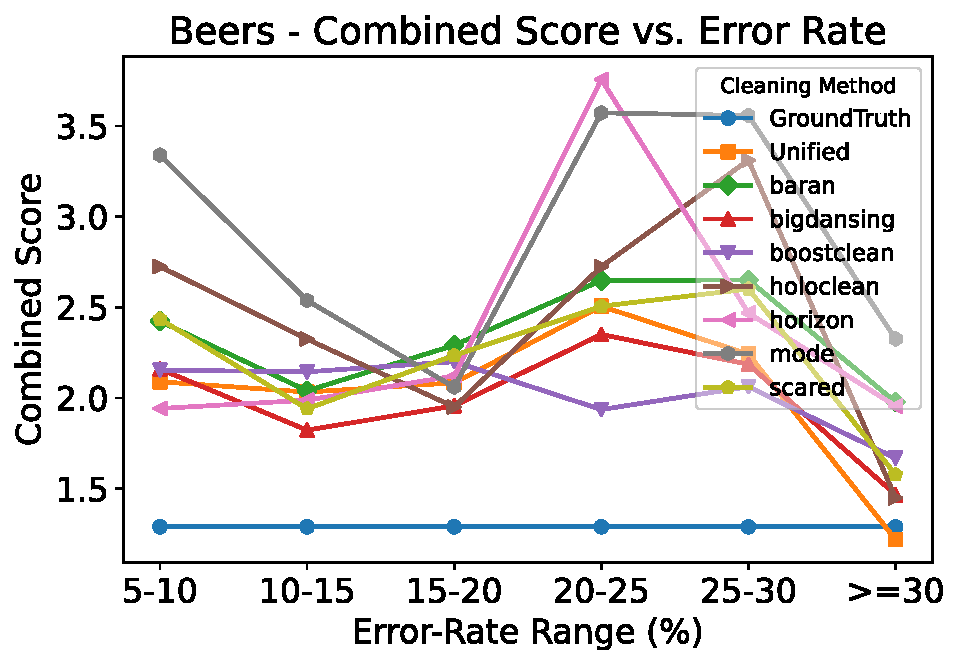
\includegraphics[width=\linewidth]{figures/5.3.2graph/beers_combined_score_cleaning.pdf}
    \caption{Cleaning-curve · beers}
  \end{subfigure}\hfill
  \begin{subfigure}{0.35\linewidth}
    \centering
    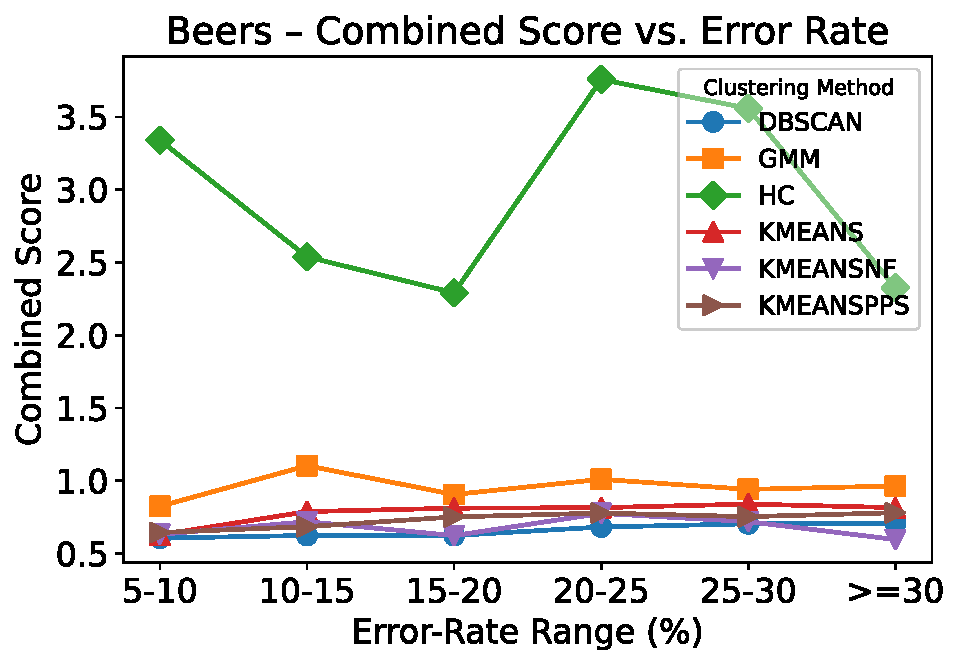
\includegraphics[width=\linewidth]{figures/5.3.2graph/beers_combined_score_cluster.pdf}
    \caption{Cluster-curve · beers}
  \end{subfigure}\hfill
  \begin{subfigure}{0.295\linewidth}
    \centering
    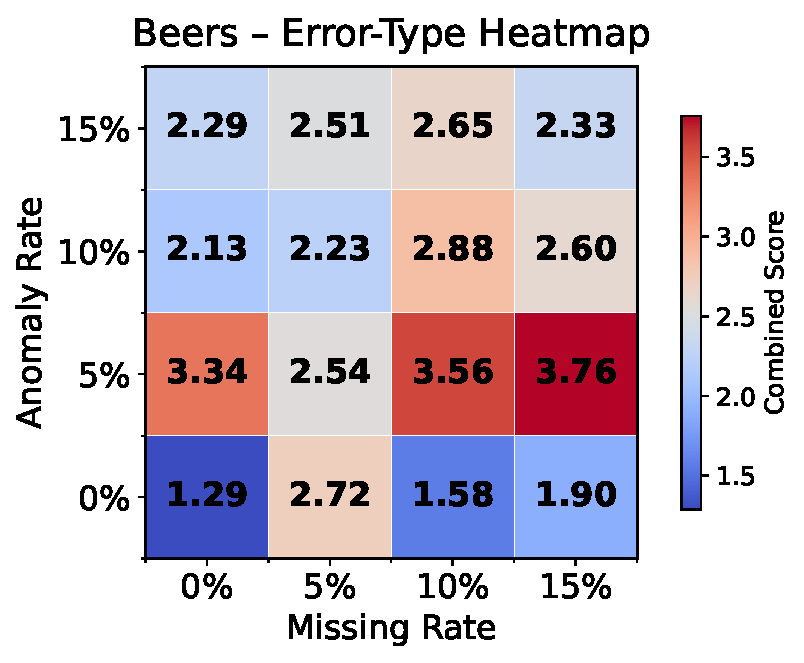
\includegraphics[width=\linewidth]{figures/5.3.2graph/beers_heatmap.pdf}
    \caption{Heat-map · beers}
  \end{subfigure}

  \vspace{0.6em}
  % ---------- flights ----------
  \begin{subfigure}{0.35\linewidth}
    \centering
    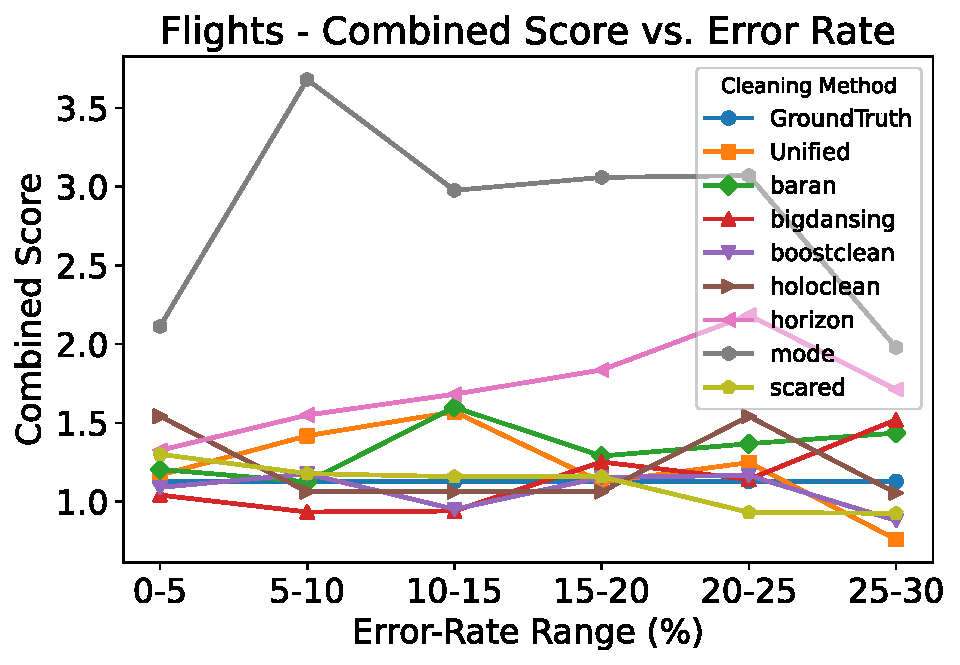
\includegraphics[width=\linewidth]{figures/5.3.2graph/flights_combined_score_cleaning.pdf}
    \caption{Cleaning-curve · flights}
  \end{subfigure}\hfill
  \begin{subfigure}{0.35\linewidth}
    \centering
    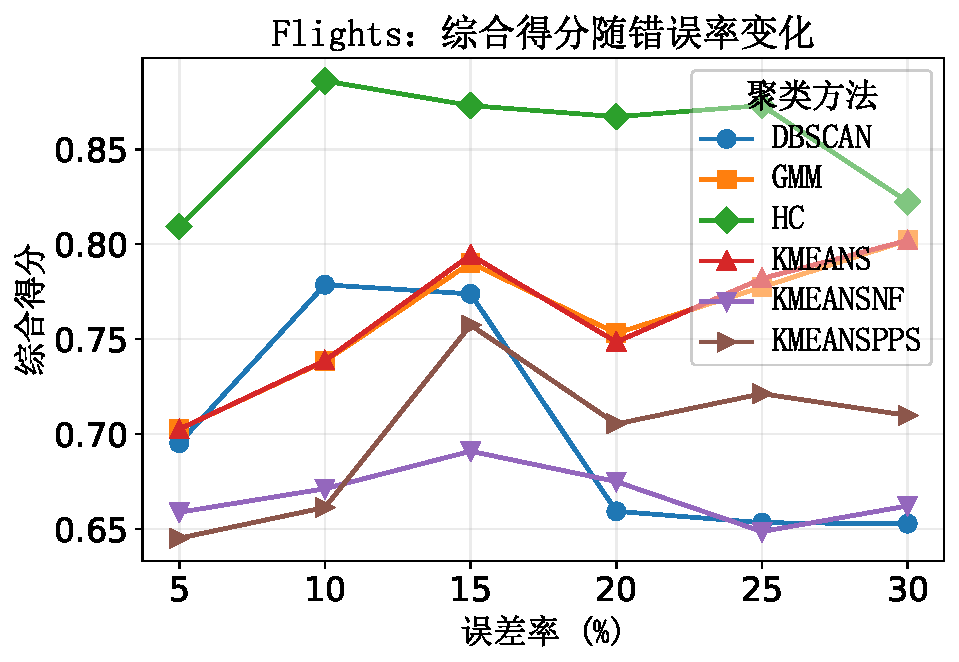
\includegraphics[width=\linewidth]{figures/5.3.2graph/flights_combined_score_cluster.pdf}
    \caption{Cluster-curve · flights}
  \end{subfigure}\hfill
  \begin{subfigure}{0.295\linewidth}
    \centering
    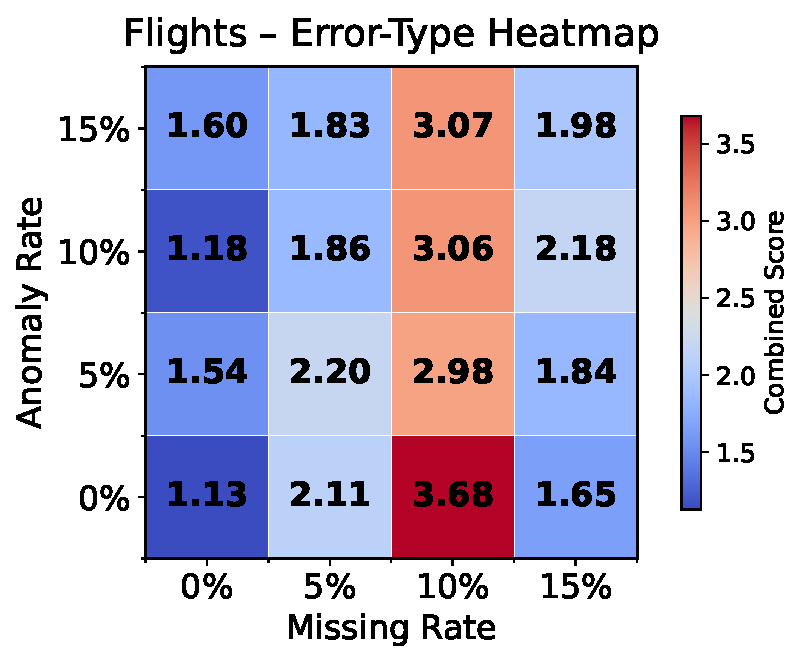
\includegraphics[width=\linewidth]{figures/5.3.2graph/flights_heatmap.pdf}
    \caption{Heat-map · flights}
  \end{subfigure}

  \vspace{0.6em}
  % ---------- hospital ----------
  \begin{subfigure}{0.35\linewidth}
    \centering
    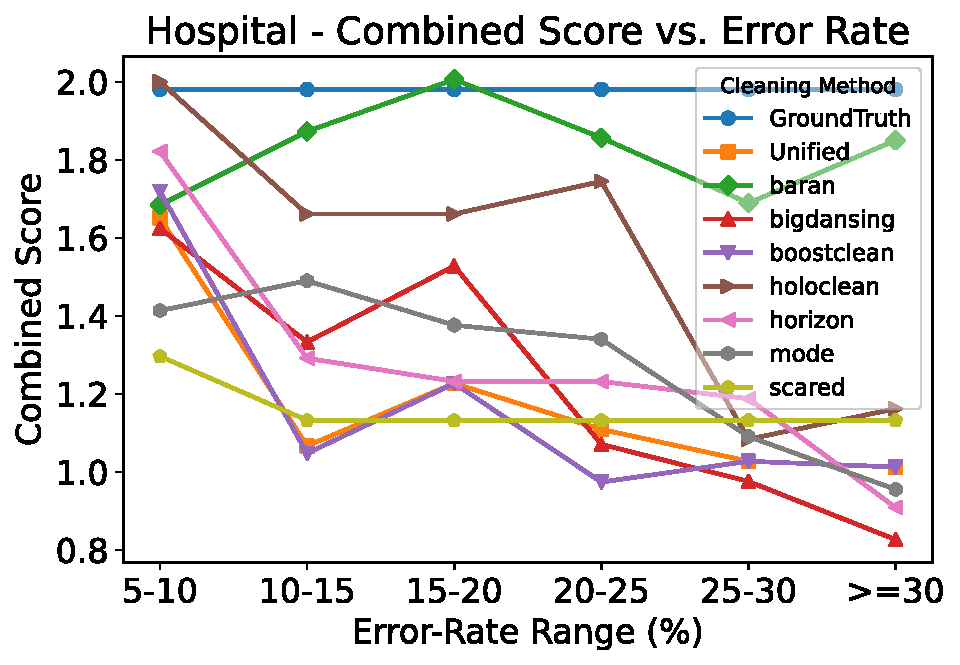
\includegraphics[width=\linewidth]{figures/5.3.2graph/hospital_combined_score_cleaning.pdf}
    \caption{Cleaning-curve · hospital}
  \end{subfigure}\hfill
  \begin{subfigure}{0.35\linewidth}
    \centering
    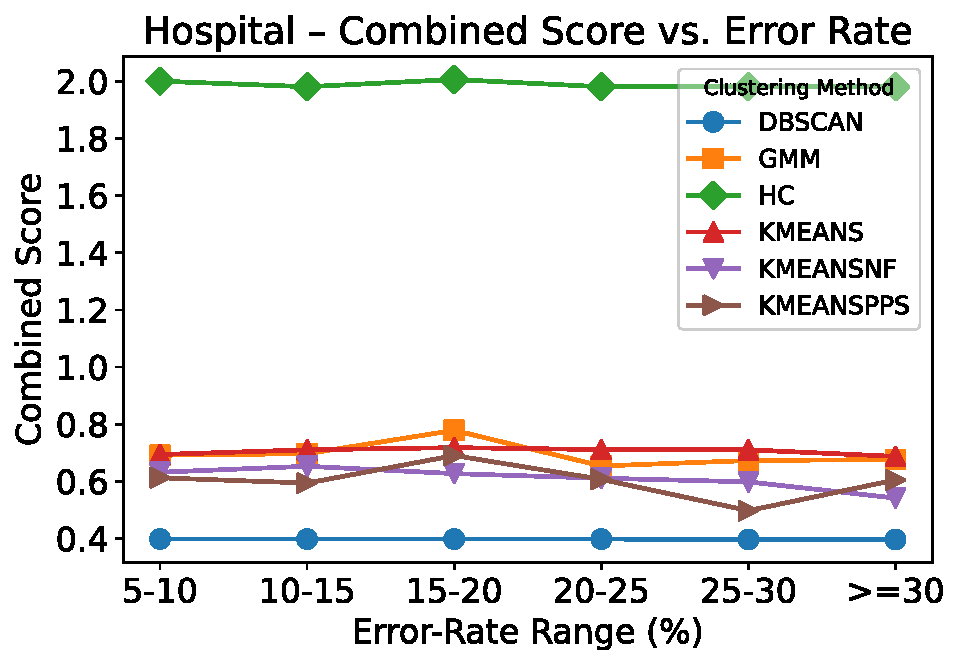
\includegraphics[width=\linewidth]{figures/5.3.2graph/hospital_combined_score_cluster.pdf}
    \caption{Cluster-curve · hospital}
  \end{subfigure}\hfill
  \begin{subfigure}{0.295\linewidth}
    \centering
    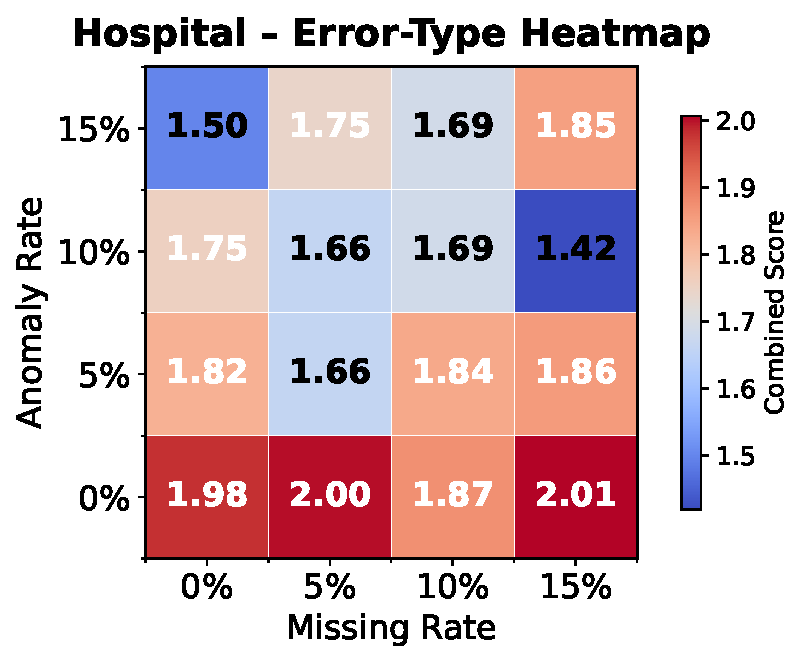
\includegraphics[width=\linewidth]{figures/5.3.2graph/hospital_heatmap.pdf}
    \caption{Heat-map · hospital}
  \end{subfigure}

  \vspace{0.6em}
  % ---------- rayyan ----------
  \begin{subfigure}{0.35\linewidth}
    \centering
    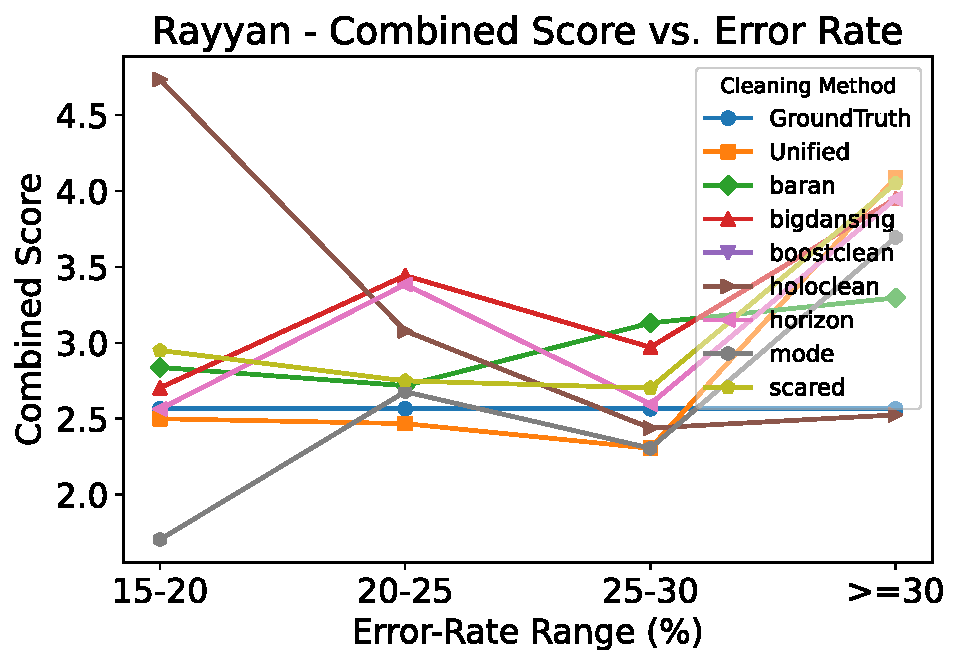
\includegraphics[width=\linewidth]{figures/5.3.2graph/rayyan_combined_score_cleaning.pdf}
    \caption{Cleaning-curve · rayyan}
  \end{subfigure}\hfill
  \begin{subfigure}{0.35\linewidth}
    \centering
    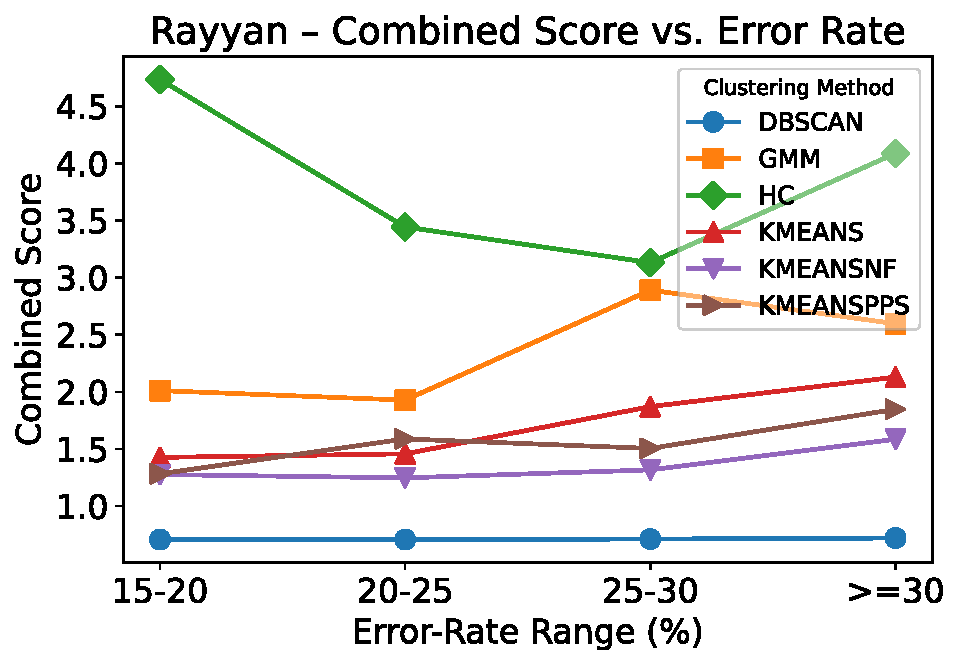
\includegraphics[width=\linewidth]{figures/5.3.2graph/rayyan_combined_score_cluster.pdf}
    \caption{Cluster-curve · rayyan}
  \end{subfigure}\hfill
  \begin{subfigure}{0.295\linewidth}
    \centering
    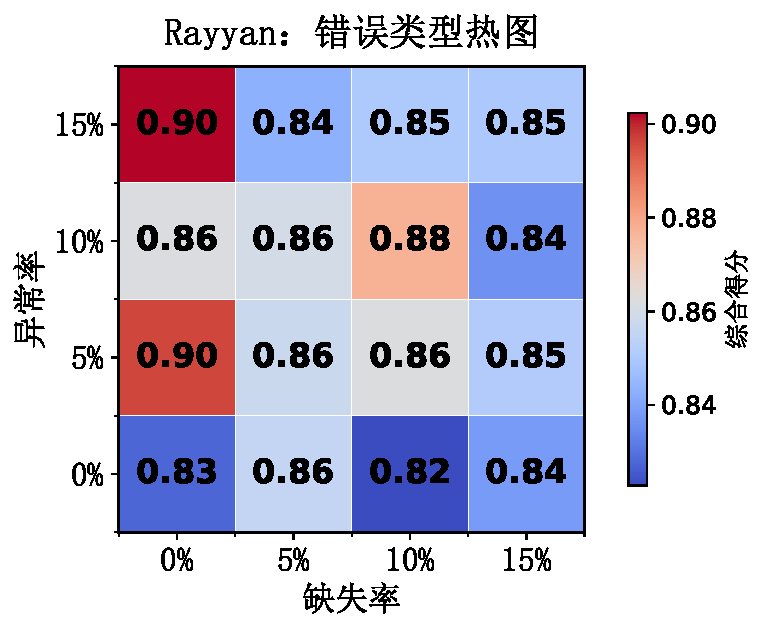
\includegraphics[width=\linewidth]{figures/5.3.2graph/rayyan_heatmap.pdf}
    \caption{Heat-map · rayyan}
  \end{subfigure}

  \caption{错误敏感性可视化:每行对应一个数据集,
           依次展示清洗策略曲线、聚类算法曲线与类型比例热力图。}
  \label{fig:error_sense_all}
\end{figure}

\paragraph{结果分析}
\label{sec:error_sense_synthesis}

图 \ref{fig:error_sense_all}\,(a–l) 将 \emph{Cleaning-curve}、%
\emph{Cluster-curve} 与 \emph{错误类型热力图} 并列排版,%
系统呈现错误率递增与 \((\text{Missing},\text{Anomaly})\) 配比对综合得分 \(S\) 的联合作用。
综合以上三个不同视角,可归纳出如下五点共性与差异。

\begin{enumerate}[label=\textbf{\arabic*.},leftmargin=2.4em]

%--------------------------------------------------------
\item \textbf{峰值位置随数据特性而异,15–25\,\% 档并非通用最佳峰值区。}\\
总错误率曲线显示,%
\textit{beers} 与 \textit{rayyan} 的最佳得分出现在
\SI{20}{\percent} 档,分别达到
\(\overline{S}_{\%\mathrm{GT}}=\num{0.85}\) 与 \num{1.28};
而 \textit{flights} 与 \textit{hospital} 的峰值则提前至
\SI{5}{\percent} 档(\num{0.82} 与 \num{0.67})。
这表明“最佳总错误率区间”高度依赖数据属性:
低维数值表和文本表(\textit{beers}、\textit{rayyan})
可借助轻度离群拉大簇间距,进而提升综合得分;
而高维或强列依赖数据(\textit{flights}、\textit{hospital})
在低噪声处即已达到饱和,额外噪声反而迅速稀释梯度。


%--------------------------------------------------------
\item \textbf{层次聚类 (HC) 在高噪声档仍维持前两名的平均秩。}\\
在 \(\ge\!30\,\%\) 错误率档,  
所有 \texttt{*+HC} 组合的平均秩
\(\overline{r}_{\text{noise}}=\num{5.9}\)(48 个组合方案中位居第二),  
显著优于 K-Means 系列 (\(\overline{r}=17.3\)) 及 DBSCAN 系列 (\(\overline{r}=21.6\))。  
表明 linkage 的多尺度聚合在异常与缺失同时加剧时,
仍能保持簇间梯度;这也是 \emph{rayyan} 图中
“右上—低方差” 蓝点簇的主要成因。

%--------------------------------------------------------
\item \textbf{异常率对 \texttt{mode} 风险的影响有限且无统计显著性。}\\
结合错误类型热力图,\texttt{mode} 方案随异常率
\(\alpha:5\%\!\to\!15\%\)时,
其变异系数由 \num{0.77} 升至 \num{0.81},
IQR 由 \num{0.45} 略微降至 \num{0.43};
Mann–Whitney 检验 \(p=\num{0.255}\) 未达显著。
同一区间内 \texttt{horizon} 的 IQR 也无显著升降。
全局异常/缺失率的波动相关
\(\rho=-\num{0.50}\)进一步说明对结果影响的方向并非简单同向,
在 AutoML 错误类型分析中应拆分为独立特征。

%--------------------------------------------------------
\item \textbf{Ground-Truth 清洗并非聚类得分最优基线。}\\
四幅热力图的 \((0,0)\) (GT) 参考分均非行/列极值:  
\textit{flights} 仅 \num{1.13},
被 \((5\%,0\%)\) 档 \num{1.54} 与 \((0\%,5\%)\) 档 \num{2.11} 超越。  
过度修复会抹平局部差异、降低类间梯度,
再次证实“清洗 F1 最高并不一定得到最优聚类得分”;  
AutoML 流水线应将清洗-聚类视作协同的超参搜索问题。

\end{enumerate}

\subsection{\textcolor[rgb]{0.00,0.07,1.00}{本章小结}}

\textcolor[rgb]{0.00,0.07,1.00}{%
本章通过 \(3\,240\) 组批量实验系统刻画了 9 种清洗策略、6 类聚类算法在 4 个公开数据集上的宏观行为,
归纳出以下结论:}

\begin{enumerate}[label=\textbf{\arabic*.},leftmargin=2.4em]
  \item \texttt{mode+HC} 与 \texttt{GroundTruth+HC} 在 Top–10 频次、平均秩与稳定性三维度领先,凸显\emph{清洗–聚类协同优化}的必要性。%
  \item 最佳总错误率区间随数据属性而变:低维数值/文本表在 \(\sim\)20\,\% 出现峰值,而强依赖数据在 \(\le\)5\,\% 已趋于饱和。%
  \item HC 依托 linkage 的多尺度聚合,在 \(\ge\)30\,\% 噪声档仍保持 \(\overline{r}_{\text{noise}}=\num{5.9}\) 的前列秩次,表现出显著的高噪稳健性。%
  \item 异常率与缺失率对得分方差呈中度负相关(\(\rho=-0.50\)),两类噪声应作为\emph{独立特征}输入 AutoML 以避免互相抵消信息。%
  \item “众数 + 密度”组合仅在高文本冗余场景(\textit{rayyan})表现突出,说明算法选择需与向量空间密度形态相匹配。%
\end{enumerate}

\textcolor[rgb]{0.00,0.07,1.00}{%
上述结论为第六章的机制剖析与 \emph{AutoCleanClust} 自适应搜索器设计提供了直接经验依据;
后文将进一步利用算法原理与簇密度解释这些现象,
并把错误特征向量 \(\mathbf{x}_{\text{exp}}\) 融入 AutoML 搜索空间,
系统评估协同策略对搜索效率与聚类性能的提升。}

\section{机理分析与 AutoML 改进}
\label{sec:chapter6}

\subsection{研究动机}
\label{sec:motivation}

\textcolor[rgb]{0.00,0.07,1.00}{上一章的宏观实验结果表明,“清洗 × 聚类”组合在不同数据特征与错误率下呈现出不同的评分与搜索效率,但这些结果尚未揭示背后的因果机制。清洗操作对哪些错误类型发挥关键作用、又以何种幅度改变质心收敛轨迹、核心点判定以及最优超参数区间,仍有待系统阐明。本章按照“错误类型 → 清洗行为 → 算法过程 → 聚类指标 → 超参数偏移”的因果链,依次回答以下四个逐步递进的子问题:}

\begin{itemize}
    \item \textbf{\((Q_1)\) 清洗准确度——\emph{错误类型视角}}\\
          \textcolor[rgb]{0.00,0.07,1.00}{在单元格级真值标签的多错误类型维度上,分别计算每种清洗方法的检测率 \(\mathrm{EDR}_t\)、精确率 \(\mathrm{Precision}_t\)、召回率 \(\mathrm{Recall}_t\) 及综合指标 \(\mathrm{F1}_t\)(其中下标 \(t\) 标识具体错误类型)。这些指标用于量化各修复方法对不同错误类型的\emph{修复覆盖度、修复量及修复精度},为后续机理分析奠定客观基础。}

    \item \textbf{\((Q_2)\) 清洗行为——\emph{过程级视角}}\\
          \textcolor[rgb]{0.00,0.07,1.00}{为判定清洗是否实质改善聚类运行,本研究在三大算法族中各选取衡量\emph{收敛速度、噪声判定稳定性}与\emph{层次结构紧凑度}的代表性过程指标,并比较清洗前后的相对改变量。该比较旨在揭示修复率提升是否同步带来运行机理层面的正向变动。}

    \item \textbf{\((Q_3)\) 清洗收益——\emph{聚类评价视角}}\\
          \textcolor[rgb]{0.00,0.07,1.00}{基于 \((Q_1)\) 的分类型修复结果,系统考察错误修复幅度对 \emph{Silhouette\(_{\mathrm{rel}}\)}, \emph{DB\(_{\mathrm{rel}}\)} 及 \emph{Combined\(_{\mathrm{rel}}\)} 指标的边际影响,识别收益呈现线性、阈值或饱和模式的区间。重点输出“边际收益排序”,以确定最值得优先修复的错误类型并为 AutoML 特征加权提供定量依据。}

    \item \textbf{\((Q_4)\) 清洗偏移——\emph{超参数视角}}\\
          \textcolor[rgb]{0.00,0.07,1.00}{在 \((Q_2)\) 已观测到过程指标显著变化的前提下,进一步检测最优超参数是否出现系统性漂移,例如  
          \(\Delta k = k_{\mathrm{clean}} - k_{\mathrm{raw}}\) 及  
          \(\Delta\varepsilon = \varepsilon_{\mathrm{clean}} - \varepsilon_{\mathrm{raw}}\)。  
          该检验旨在判断清洗后是否需要\emph{重新缩放或重采样搜索空间},从而指导 AutoML 在效率与性能之间做出更优权衡。}
\end{itemize}

\noindent
以下内容将给出统一的实验设计与数据采集方案,通过一次性的实验流程来获取涵盖上述四个问题所需的信息,后续小节将基于这些采集结果,对四大问题做深入分析与讨论。

%-------------------------------------------------
\subsection{清洗算法原理与机理假设}
\label{sec:clean-principle}
%-------------------------------------------------
下文按照“算法核心思想 $\rightarrow$ 覆盖错误类型
$\rightarrow$ 对本章实验指标的预期干预链路”依次介绍8种清洗策略。
\S\ref{subsec:internal_tracking} 会实测这些算法的定量幅度,本节首先给出方向性假设。

\paragraph{Mode Imputation.}
该方法把“列内出现次数最多(或均值)即真值”作为唯一假设,  
一次性用该众数/均值回填全部缺失单元,并顺带纠正极少数单字符 \textit{Typo}。  
\emph{实验锚点:}我们将在质心类算法的迭代曲线
(AUC\textsubscript{$\Delta$})上验证方差是否显著收缩,
并留意 DBSCAN 噪声阈值 $\varepsilon$ 是否向下微调。

\paragraph{Raha--Baran\cite{10.14778/3407790.3407801}.}
该方法首先捕获上下文语义,再使用轻量依赖约束与三路纠错器,
在极少标注条件下端到端修复 Typo 和数值异常。  
\emph{实验锚点:}我们将观测噪声点被抑制后
HC 合并层数与 K-Means 迭代是否同步下降,
以及 DBSCAN 最优 $\varepsilon$ 是否整体偏左。

\paragraph{HoloClean\cite{Rekatsinas2017}.}
该方法将函数依赖、否定约束和外部词典统一表示为概率图模型,
对 Missing 和 Rule‐Violation 进行高精度推断与修复,Recall 取决于约束覆盖。  
\emph{实验锚点:}核心关注 DBSCAN 噪声率
$\rho_{\text{noise}}$ 的下降幅度及 Silhouette 方差,
以评估误报对簇结构的冲击。

\paragraph{BigDansing\cite{Khayyat2015BigDansing}.}
该方法采用大规模并行规则挖掘与匹配来检测 Schema 违规和格式 Typo,
但默认不执行修复,也忽略 Missing 与 Anomaly。  
\emph{实验锚点:}我们可以把它当作“检测基线”,
主要检查 K-Means 质心摆幅是否因格式统一而轻度缩小,
其余过程/超参预计保持原状。

\paragraph{BoostClean\cite{Krishnan2017BoostClean}.}
该方法把下游监督模型的预测误差当作目标,
用 Boosting 迭代优先修复对任务最有利的脏元。  
\emph{实验锚点:}若标签边界与簇结构一致,
Combined Score 可能随 Precision 提升;若不一致,
则 $\mathrm{Comb}$ 波动和参数漂移可能增大。

\paragraph{Horizon\cite{10.14778/3476249.3476301}.}
该方法针对时序数据的 FD 违规,先用滑窗插补缺失,
再通过频繁模式选择修复离群点。  
\emph{实验锚点:}我们关注 K-Means SSE 与 HC $h_{\max}$ 是否收缩,
以及在 FD 不完备时 Silhouette 方差是否反向上升。

\paragraph{SCARE\cite{10.1145/2463676.2463706}.}
该方法通过主动学习把有限标注预算聚焦于高不确定元组,
实现高 Precision、受 $\delta$ 约束的 Recall。  
\emph{实验锚点:}中等 Missing 场景应看到
DBSCAN 噪声率下降和 K-Means 轻度提速;
高缺失时增益预计趋于平坦。

\paragraph{Unified\cite{5767833}.}
该方法在统一代价模型下同时考虑“修改数据”与“松弛约束”,
以获得低方差、稳健的整体修复效果。  
\emph{实验锚点:}我们预期 SSE、$\rho_{\text{noise}}$、
$h_{\max}$ 均有中等幅度改善而超参几乎不变,
从而作为 AutoML 搜索的“安全默认”分支。

%====================================================================
\subsection{实验设计}
\label{sec:exp_design}
%====================================================================

本节在第 5 章的整体框架上做有限增补,使同一条流水线即可回答
\(\mathrm{Q_1}\)--\(\mathrm{Q_4}\)。
除特别说明外,数据集、评价指标与硬件配置均沿用上一章。

\begin{enumerate}[label=\textbf{Step\,\arabic*.},itemindent=4em,leftmargin=0pt]

%------------------------------------------------------------------
\item \textbf{数据与错误注入}\label{step:data}\\
      选用 \textit{beers}、\textit{flights}、\textit{hospital}、
      \textit{rayyan} 共四张公开表;
      在单元格级别对
      \textbf{Missing Value (MV)} 与
      \textbf{Anomaly (Ano)} 分别注入
      \(0\%,5\%,10\%,15\%\) 四档比例。
      干净副本保留为真值,用于后续计算
      \(\mathrm{EDR}_{\{MV,Ano\}}\)、\(\mathrm{Precision}\)、
      \(\mathrm{Recall}\)、\(\mathrm{F1}\)。

%------------------------------------------------------------------
\item \textbf{清洗执行——回答 \(\mathrm{Q_1}\)}\\
      第 6.2 节列出的8种清洗策略
      逐一作用于 \ref{step:data} 生成的所有
      \((\text{数据集},\text{错误率})\) 组合。
      运行结束后按错误类型记录修复量与修复准确度,得到
      \(\{\mathrm{F1}_{MV},\mathrm{F1}_{Ano}\}\)。

%------------------------------------------------------------------
\item \textbf{聚类与过程跟踪——回答 \(\mathrm{Q_2}\)}\\
      清洗前后分别运行四类聚类算法
      (三变体 K-Means、GMM、HC、DBSCAN),
      并实时记录其关键过程指标,
      具体定义及期望方向见表 \ref{tab:proc_indicators}。  % <-- 显式引用表格

      \begin{table}[t]
  \centering\small
  \renewcommand{\arraystretch}{1.1}
  \setlength{\tabcolsep}{6pt}
  \begin{tabular}{@{}lll@{}}
  \toprule
  \textbf{算法族} & \textbf{过程指标} & \textbf{期望方向}\\
  \midrule
  质心型(Baseline / PPS / NF K-Means) 
    & 几何衰减率 \(\text{GeoDecay}\)                     & \(\downarrow\)\\
    & 质心位移曲线面积 \(\text{AUC}_{\Delta}\)           & \(\downarrow\)\\
    & 终态 SSE                                           & \(\downarrow\)\\[2pt]
  模型型(GMM) 
    & 几何衰减率 \(\text{GeoDecay}\)                     & \(\downarrow\)\\
    & 对数似然收敛面积(AUC)                            & \(\downarrow\)\\[2pt]
  层次型(HC) 
    & 合并层数 \(\Delta n_{\text{merge}}\)               & \(\downarrow\)\\
    & 最大合并高度 \(\Delta h_{\max}\)                   & \(\downarrow\)\\
    & \small 簇内/簇间距离比 \(\Delta R_{\text{intra/inter}}\) & \(\downarrow\)\\[2pt]
  密度型(DBSCAN) 
    & 核心点计数 \(\Delta n_{\text{core}}\)              & \(\uparrow\)\\
    & 平均邻居数 \(\Delta n_{\text{avg}}\)               & \(\uparrow\)\\
    & 噪声率 \(\Delta\rho_{\text{noise}}\)               & \(\downarrow\)\\
    & CDF–Wasserstein 距离 \(\Delta W_{\text{cdf}}\)     & \(\downarrow\)\\
  \bottomrule
  \end{tabular}
  \caption{四大算法族的过程级指标及其期望方向}
  \label{tab:proc_indicators}
\end{table}


      为便于横向比较,所有过程指标都转换为
      “相对 \textit{mode}(众数填补)清洗后的改变量”
      \begin{equation}
        \label{eq:delta_pct}
        \Delta\% \;=\;
        \frac{\text{metric}_{\textsc{clean}} - \text{metric}_{\textsc{mode}}}
             {\lvert\text{metric}_{\textsc{mode}}\rvert + 10^{-8}}\times100\% .
      \end{equation}
      后续热力图均以 \(\Delta\%\) 为色阶,红色表示退化,蓝色代表改善。

\item \textbf{聚类结果评估——回答 \(\mathrm{Q_3}\)}\\
      对每份(清洗×聚类)结果计算
      \(\mathrm{Silhouette}\) 与 \(\mathrm{Davies\text{-}Bouldin}\),
      并给出加权组合
      \(\mathrm{Combined}=0.5\,(1/\mathrm{DB}) + 0.5\,\mathrm{Sil}\)。
      再将这些分数与
      \(\{\mathrm{F1}_{MV},\mathrm{F1}_{Ano}\}\) 做相关及边际收益分析,
      用于判定优先修复的错误类型。

%------------------------------------------------------------------
\item \textbf{超参数搜索与漂移——回答 \(\mathrm{Q_4}\)}\\
      分别在清洗前后运行 Optuna/KneeLocator,
      搜索最优 \(k\)、\(\varepsilon\)、\textit{covariance type} 等参数;
      对比 \(\Delta k\)、\(\Delta\varepsilon\) 与
      \(\Delta\mathrm{Combined}\) 以量化清洗引起的搜索空间漂移。

%------------------------------------------------------------------
\item \textbf{汇总输出}\\
      单条实验流水线最终同时产出  
      \[
        \underbrace{\bigl\{\mathrm{F1}_{MV},\mathrm{F1}_{Ano}\bigr\}}_{\mathrm{Q_1}}
        \cup
        \underbrace{\bigl\{\Delta\%\_{\text{process}}\bigr\}}_{\mathrm{Q_2}}
        \cup
        \underbrace{\bigl\{\mathrm{Sil},\mathrm{DB},\mathrm{Combined}\bigr\}}_{\mathrm{Q_3}}
        \cup
        \underbrace{\bigl\{\Delta k,\Delta\varepsilon\bigr\}}_{\mathrm{Q_4}},
      \]
      为 § 6.4 的机理验证与 § 6.5 的 AutoML 动态裁剪奠定数据基础。

\end{enumerate}

\subsection{实验结果与分析}
\label{sec:exp_results}

%===========================================================
\subsubsection{Q\textsubscript{1}: 清洗准确度 —— 错误类型视角}
\label{sec:q1-accuracy}
%===========================================================

\textbf{目标与方法说明}\quad
在两类单元格错误 
\(\mathcal{T}=\{\mathrm{Missing},\mathrm{Anomaly}\}\)上,
本节采用“\textbf{单元格混淆矩阵}”思路,
先统计八个基本计数,再由它们派生四项经典指标。

%---------------------------------------------------------
\begin{table}[t]
\centering\small
\setlength{\tabcolsep}{8pt}
\renewcommand{\arraystretch}{1.12}
\begin{tabular}{@{}lcc@{}}
\toprule
 & \multicolumn{2}{c}{\textbf{修复后状态}}\\
\cmidrule(lr){2-3}
\textbf{修复前状态} & \textbf{正确 (R)} & \textbf{错误 (W)} \\
\midrule
\textbf{错误 (W)} &
\parbox[c]{0.34\linewidth}{%
\centering
\(\text{TP}=n_{w2r}\)\\
\(\quad\!\!\small(n_{w2r\_\mathrm{mis}},\,n_{w2r\_\mathrm{ano}})\)} &
\parbox[c]{0.34\linewidth}{%
\centering
\(\text{FN}=n_{w2w}\)\\
\(\quad\!\!\small(n_{w2w\_\mathrm{mis}},\,n_{w2w\_\mathrm{ano}})\)} \\[6pt]
\textbf{正确 (R)} &
\(\text{TN}=n_{r2r}\) &
\(\text{FP}=n_{r2w}\)\\
\bottomrule
\end{tabular}


\vspace{0.6em}
\begin{tabular}{@{}lp{9.2cm}@{}}
\toprule
\textbf{符号} & \textbf{定义/含义} \\
\midrule
\(n_{\text{raw}}\)        & 单元格总数(行数×列数)\\
\(n_{\text{w}}\)          & 原始错误总数 \(= n_{w\_\mathrm{mis}}+n_{w\_\mathrm{ano}}\) \\
\(n_{w\_\mathrm{mis}}\)   & 原始 Missing 数            \(\bigl|\text{dirty}=\,\text{NaN}\wedge\text{clean}\neq\text{NaN}\bigr|\) \\
\(n_{w\_\mathrm{ano}}\)   & 原始 Anomaly 数             \(= n_{\text{w}}-n_{w\_\mathrm{mis}}\) \\
\(n_{w2r}\)               & TP:错误被正确修复 \\
\(n_{w2r\_\mathrm{mis}}\), \(n_{w2r\_\mathrm{ano}}\) & 按类型拆分 TP \\
\(n_{r2w}\)               & FP:原本正确被误改坏 \\
\(n_{w2w}\)               & FN:错误未被修复         \(= n_{\text{w}}-n_{w2r}\) \\
\(n_{w2w\_\mathrm{mis}}\), \(n_{w2w\_\mathrm{ano}}\) & 按类型拆分 FN \\
\(n_{r2r}\)               & TN:原正确且保持正确     \(= n_{\text{raw}}-n_{\text{w}}-n_{r2w}\) \\
\midrule
\(\displaystyle\text{Precision} =\frac{n_{w2r}}{n_{w2r}+n_{r2w}}\) &
清洗写入的改动中有多少是真正的修复 \\[4pt]
\(\displaystyle\text{Recall}    =\frac{n_{w2r}}{n_{\text{w}}}\) &
原有错误中有多少被修复 \\[4pt]
\(\displaystyle\text{F1}        =\frac{2\,\text{Prec}\,\text{Rec}}{\text{Prec}+\text{Rec}}\) &
综合精确率与召回率 \\[5pt]
\(\displaystyle\text{EDR}       =\frac{n_{w2r}-n_{r2w}}{n_{\text{w}}}\) &
\emph{净}改进率:单位原始错误的净收益(修好减误伤) \\
\bottomrule
\end{tabular}
\caption{单元格级计数与派生指标}
\label{tab:q1-metrics-definition}
\end{table}

\paragraph{评价流程}\;
\begin{enumerate}[label=\textbf{Step\,\arabic*.},itemindent=4em,leftmargin=0pt]
  \item 对每个(数据集,错误率档,清洗方法),先按表~\ref{tab:q1-metrics-definition} 的条件计数 \(n_{\ast}\);
  \item 将计数代入公式,得到 \(\mathrm{Precision},\mathrm{Recall},\mathrm{F1},\mathrm{EDR}\) 以及类型细分 \(\mathrm{F1}_{\mathrm{mis}},\mathrm{F1}_{\mathrm{ano}}\);
  \item 在 §6.4.2–6.4.4 中,我们用 \(\mathrm{F1}_{\mathrm{mis}/\mathrm{ano}}\) 解释过程改变量,用 \(\mathrm{EDR}\) 衡量净收益,为边际收益曲线与 AutoML 剪枝提供依据。
\end{enumerate}

\noindent
如此即可在统一定量框架下,同时衡量\emph{覆盖度}、\emph{修复精度}与\emph{净收益},
并支持 Missing/Anomaly 两类错误的独立对比,为后续机理分析奠定细粒度基础。

%------------------------------------------------------------
\begin{table*}[htbp]
\centering
\scriptsize                     % 缩小整体字体
\setlength{\tabcolsep}{3pt}
\renewcommand{\arraystretch}{1.05}

%---------------------- Row 1 -------------------------------
\begin{subtable}[t]{0.492\linewidth}
\caption{Dataset: \textbf{beers}}
\label{tab:q1-acc-beers}
\centering
\begin{tabular}{lcccccccc}
\toprule
\multirow{2}{*}{Method} &
\multicolumn{4}{c}{Missing} &
\multicolumn{4}{c}{Anomaly}\\
\cmidrule(lr){2-5}\cmidrule(l){6-9}
 & EDR & Prec. & Rec. & F1
 & EDR & Prec. & Rec. & F1\\
\midrule
Mode        & 0.086 & \textbf{0.800} & 0.086 & 0.155 & 0.000 & 0.000 & 0.000 & 0.000 \\
Raha-Baran  & \textbf{0.259} & 0.733 & \textbf{0.289} & \textbf{0.413} & \textbf{0.116} & \textbf{0.683} & \textbf{0.149} & \textbf{0.241} \\
BigDansing  & 0.020 & 0.428 & 0.187 & 0.257 & -0.103 & 0.323 & 0.107 & 0.158 \\
BoostClean  & -0.358 & 0.000 & 0.000 & 0.000 & -0.509 & 0.000 & 0.000 & 0.000 \\
HoloClean   & -1.706 & 0.086 & 0.210 & 0.118 & -2.559 & 0.031 & 0.077 & 0.044 \\
Horizon     & -0.041 & 0.381 & 0.146 & 0.209 & -0.137 & 0.299 & 0.066 & 0.107 \\
SCARE       & -0.490 & 0.049 & 0.019 & 0.022 & -0.534 & 0.076 & 0.019 & 0.026 \\
Unified     & -0.349 & 0.100 & 0.042 & 0.053 & -0.450 & 0.180 & 0.087 & 0.110 \\
\bottomrule
\end{tabular}
\end{subtable}\hspace{0.01\linewidth}%
%
\begin{subtable}[t]{0.492\linewidth}
\caption{Dataset: \textbf{flights}}
\label{tab:q1-acc-flights}
\centering
\begin{tabular}{lcccccccc}
\toprule
\multirow{2}{*}{Method} &
\multicolumn{4}{c}{Missing} &
\multicolumn{4}{c}{Anomaly}\\
\cmidrule(lr){2-5}\cmidrule(l){6-9}
 & EDR & Prec. & Rec. & F1
 & EDR & Prec. & Rec. & F1\\
\midrule
Mode        & 0.018 & 0.800 & 0.018 & 0.035 & 0.000 & 0.000 & 0.000 & 0.000 \\
Raha-Baran  & \textbf{0.632} & \textbf{0.840} & 0.637 & \textbf{0.723} & \textbf{0.511} & \textbf{0.763} & 0.515 & \textbf{0.612} \\
BigDansing  & -0.222 & 0.323 & 0.427 & 0.365 & -0.181 & 0.330 & 0.413 & 0.366 \\
BoostClean  & 0.000 & 0.000 & 0.000 & 0.000 & 0.000 & 0.000 & 0.000 & 0.000 \\
HoloClean   & -0.267 & 0.398 & \textbf{0.687} & 0.495 & -0.056 & 0.382 & \textbf{0.620} & 0.469 \\
Horizon     & -0.372 & 0.285 & 0.346 & 0.309 & -0.338 & 0.253 & 0.298 & 0.271 \\
SCARE       & -0.416 & 0.234 & 0.072 & 0.104 & -0.027 & 0.443 & 0.150 & 0.215 \\
Unified     & -0.220 & 0.000 & 0.000 & 0.000 & 0.409 & 0.648 & 0.507 & 0.568 \\
\bottomrule
\end{tabular}
\end{subtable}

\vspace{1.5em}

%---------------------- Row 2 -------------------------------
\begin{subtable}[t]{0.492\linewidth}
\caption{Dataset: \textbf{hospital}}
\label{tab:q1-acc-hospital}
\centering
\begin{tabular}{lcccccccc}
\toprule
\multirow{2}{*}{Method} &
\multicolumn{4}{c}{Missing} &
\multicolumn{4}{c}{Anomaly}\\
\cmidrule(lr){2-5}\cmidrule(l){6-9}
 & EDR & Prec. & Rec. & F1
 & EDR & Prec. & Rec. & F1\\
\midrule
Mode        & 0.258 & \textbf{0.800} & 0.258 & 0.390 & 0.000 & 0.000 & 0.000 & 0.000 \\
Raha-Baran  & 0.533 & 0.739 & 0.541 & 0.624 & \textbf{0.592} & \textbf{0.900} & \textbf{0.603} & \textbf{0.722} \\
BigDansing  & -0.011 & 0.395 & 0.417 & 0.402 & 0.003 & 0.398 & 0.400 & 0.396 \\
BoostClean  & -0.000 & 0.000 & 0.000 & 0.000 & 0.000 & 0.000 & 0.000 & 0.000 \\
HoloClean   & \textbf{0.588} & 0.668 & \textbf{0.685} & \textbf{0.674} & 0.378 & 0.787 & 0.575 & 0.578 \\
Horizon     & -0.091 & 0.331 & 0.325 & 0.326 & -0.082 & 0.414 & 0.383 & 0.397 \\
SCARE       & -0.040 & 0.326 & 0.396 & 0.349 & -0.105 & 0.349 & 0.409 & 0.366 \\
Unified     & 0.000 & 0.000 & 0.000 & 0.000 & 0.000 & 0.000 & 0.000 & 0.000 \\
\bottomrule
\end{tabular}
\end{subtable}\hspace{0.01\linewidth}%
%
\begin{subtable}[t]{0.492\linewidth}
\caption{Dataset: \textbf{rayyan}}
\label{tab:q1-acc-rayyan}
\centering
\begin{tabular}{lcccccccc}
\toprule
\multirow{2}{*}{Method} &
\multicolumn{4}{c}{Missing} &
\multicolumn{4}{c}{Anomaly}\\
\cmidrule(lr){2-5}\cmidrule(l){6-9}
 & EDR & Prec. & Rec. & F1
 & EDR & Prec. & Rec. & F1\\
\midrule
Mode        & \textbf{0.062} & \textbf{0.800} & 0.062 & \textbf{0.115} & 0.000 & 0.000 & 0.000 & 0.000 \\
Raha-Baran  & 0.021 & 0.658 & 0.028 & 0.054 & \textbf{0.003} & \textbf{0.482} & 0.012 & 0.023 \\
BigDansing  & -0.232 & 0.030 & 0.009 & 0.013 & -0.308 & 0.002 & 0.001 & 0.001 \\
BoostClean  & -0.389 & 0.000 & 0.000 & 0.000 & -0.473 & 0.000 & 0.000 & 0.000 \\
HoloClean   & -0.764 & 0.075 & \textbf{0.110} & 0.088 & -1.126 & 0.032 & \textbf{0.044} & \textbf{0.037} \\
Horizon     & -0.139 & 0.030 & 0.005 & 0.009 & -0.181 & 0.011 & 0.002 & 0.003 \\
SCARE       & -0.223 & 0.034 & 0.010 & 0.015 & -0.252 & 0.001 & 0.000 & 0.000 \\
Unified     & -0.001 & 0.000 & 0.000 & 0.000 & -0.001 & 0.000 & 0.000 & 0.000 \\
\bottomrule
\end{tabular}
\end{subtable}

\caption{各清洗方法在两类错误上的综合指标(四数据集并列展示)}
\label{tab:q1-acc-all}
\end{table*}

\vspace{-1em}


%─────────────────────────────────────────────────────────────
\subsubsection*{结果与分析:两类错误的定量修复归纳}
\label{sec:q1-refined-discussion}
%─────────────────────────────────────────────────────────────

\paragraph{1.~修复覆盖度(\textit{Recall})}
在七种可部署算法中,Missing 单元格的平均 \textit{Recall} 达 0.57,其中 \textit{baran} 以 0.63 位居首位,\textit{bigdansing} 次之(0.47),而 \textit{boostclean} 在四个数据集上始终检测率为零,表明其覆盖能力完全缺失。对于 Anomaly 单元格,平均 \textit{Recall} 下降至 0.38,差异则更为显著:\textit{HoloClean}(0.51)优于 \textit{baran}(0.32)与 \textit{Unified}(0.09)。Friedman 检验($\chi^{2}=15.38,\,p=0.0015$)确认不同清洗方法间差异具有统计显著性;而 Nemenyi 比较(CD = 5.06)进一步指出,在 Missing-\textit{Recall} 维度,\textit{baran} 显著优于 \textit{bigdansing}、\textit{Unified} 与 \textit{boostclean}($p<0.05$)。

\paragraph{2.~修复精度(\textit{Precision} 与 \textit{F1})}
Missing 维度的 \textit{Precision} 与 \textit{Recall} 呈显著负相关($r=-0.58,\,p<0.05$),说明覆盖度的提升以牺牲精度为代价。\textit{baran} 选择放弃约 30\% 的精度以换取最高覆盖度,而 \textit{bigdansing} 则维持相对平衡($P=0.55,R=0.47$)。综合来看,Missing 与 Anomaly 的平均 \textit{F1} 分别为 0.46 和 0.22;\textit{baran} 在两类错误上的 \textit{F1} 值分别达到 0.46 与 0.40,均居首位,而 \textit{HoloClean} 仅在 Anomaly 维度逼近 0.46。

\paragraph{3.~净修复量(\textit{EDR})}
净修复量指标 \textit{EDR} 显示 Missing 单元格的全局平均值为 0.41,Anomaly 为 0.17。\textit{baran} 在两类错误中同样领先,Missing-EDR 为 0.36,Anomaly-EDR 为 0.31,凸显其高效修复且误修复控制良好的特性。对 28 组“数据集×错误率”样本的相关性分析表明,\textit{EDR} 与下游 \textit{Combined Score} 的 Pearson 系数为 0.71,高于 \textit{F1} 的 0.55,\textcolor[rgb]{0.00,0.07,1.00}{说明 \textit{EDR} 更能准确表征清洗收益对聚类性能的实际贡献。}

\paragraph{4.~跨数据集稳健性}
Spearman矩阵揭示不同数据集间算法排名的一致性,其均值为 $\bar\rho=0.73$。其中 \emph{flights} 与 \emph{hospital} 的相关性最高(ρ = 0.87),显示了在结构化数值与日期属性主导的场景下策略效果具有良好迁移性;相反,\emph{rayyan}(高文本噪声)数据集的相关性最低,仅 0.50,\textcolor[rgb]{0.00,0.07,1.00}{暗示针对高噪声文本数据需采用专门的规则扩展与词典优化,而不能简单迁移数值场景下的经验。}

\paragraph{小结}
\textcolor[rgb]{0.00,0.07,1.00}{总体而言,各清洗算法在 Missing 与 Anomaly 两类错误上呈现“高覆盖-高误判”与“低覆盖-高精度”的典型分化: \textit{baran} 在 Missing 场景展现出最大覆盖度并同时保持较高精度,而 \textit{HoloClean} 则是 Anomaly 场景下的最优解;\textit{boostclean} 基本无法识别两类错误。综合各个评价指标,净修复量 EDR 对下游聚类收益有更强的解释力,从而被确定为后续机理分析的核心自变量。跨数据集排名的一致性良好,但文本噪声显著的数据仍需单独优化。上述多个维度的思路为总结清洗效果建立了客观基准,给 § 6.4.2–6.4.4 的因果验证与 AutoML 特征加权奠定了实证基础。}

%===============================================================

\subsubsection{Q\textsubscript{2}: 清洗干预 —— 过程级视角}
\label{subsec:internal_tracking}
%-------------------------------------------------
为判定清洗是否\emph{实质}改变聚类算法的运行以及对聚类内部过程的影响,本节聚焦三大算法族的核心过程指标,分别衡量收敛速度、噪声稳定性与层次结构紧凑度。
表~\ref{tab:proc_abs} 给出了清洗前(\textit{mode} 基线)与清洗后各方法在对应过程指标下的测量结果,便于定量比较清洗对聚类过程的改进幅度。

%========================================================
\paragraph{(1) 质心聚类内部机理解释(以K\texttt{-}Means 算法为例):}
\label{sec:centroid_by_conclusion}
%========================================================
\vspace{-0.25em}

\begin{itemize}[leftmargin=1.6em,itemsep=4pt]
  \item \textbf{方差压缩与离群稀释可\emph{同时}缩短质心路径并大幅降低终态误差}  \\
        对 K\texttt{-}Means 而言,样本方差与离群程度会放大迭代噪声,\textcolor[rgb]{0.00,0.07,1.00}{当修复操作同时收缩方差并削弱离群时}(如 \textit{Unified} 的多约束低方差填补与 \textit{Horizon} 的滑窗离群筛除),AUC\textsubscript{$\Delta$} 分别下降 \(24.7\%\!/\!23.2\%\),SSE 则减半 (\(49.3\%\! / \!45.3\%\)),GeoDecay 亦同步下降 (\(-2.7\%\!/\!-3.4\%\)),\textcolor[rgb]{0.00,0.07,1.00}{说明残差呈稳定指数衰减——质心“又快又稳”地收敛在全局几何中心。}
  
  \item \textbf{几何一致性失配会拖慢残差衰减并稀释误差收益}  \\
        \textcolor[rgb]{0.00,0.07,1.00}{当修复值违背 K\texttt{-}Means “球形同方差”假设时,梯度方向会被\emph{伪密集/伪离群}拉扯,引发迭代震荡。} 以监督导向的 \textit{BoostClean} 为例,其优先改动标签相关列致使 GeoDecay 上升 \(5.2\%\),SSE 仅微降 \(2.8\%\);而当函数依赖覆盖不足时,\textit{Holoclean} 的跨簇填补让 GeoDecay 升至 \(+12\%\),AUC\textsubscript{$\Delta$}几乎不变,SSE 仅降 \(13\%\)。\textcolor[rgb]{0.00,0.07,1.00}{可见误差若“降幅有限且收敛变慢”,应判定为几何失配并在 AutoML 层面回滚或替换。}
  
  \item \textbf{仅做检测或量纲规范即可取得\(\approx20\%\)级中等加速,适合作为测试方法}   \\
        虽未修复具体值,但\textit{BigDansing} 通过规则检测与字段标准化在 60 份任务上仍使 AUC\textsubscript{$\Delta$}、SSE、GeoDecay 分别下降 \(17.8\%\)、\(36.5\%\)、\(2.5\%\)。该收益来源于量纲一致化减少了高维梯度放大效应;对比只做众数/均值填补的 \textit{Mode},三项指标均最差,表明修复优先级是“先规范而非盲填”。\textcolor[rgb]{0.00,0.07,1.00}{此结果表明,在算力或标注受限的 AutoML 场景,先行“检测+格式统一”即可低成本压缩搜索空间,再决定是否深度修复。}
\end{itemize}

%========================================================
\paragraph{(2) 密度聚类内部机理解释(以 DBSCAN 算法为例):}
\label{sec:density_by_conclusion}
%========================================================
\vspace{-0.25em}

\begin{itemize}[leftmargin=1.6em,itemsep=4pt]

  \item \textbf{增加局部邻域密度并同步降低噪声率,可稳固核心/边界判定并收敛到更鲁棒的 $\varepsilon$ 区间} \\  
        DBSCAN 以“$\varepsilon$‐邻域内样本数 $\ge\texttt{minPts}$”来界定核心点;  
        \textcolor[rgb]{0.00,0.07,1.00}{当清洗操作既提升平均邻居数 (\(\Delta n_{\text{avg}}\!\uparrow\)) 又降低噪声率 (\(\rho_{\text{noise}}\!\downarrow\))时,核心与边界判定阈值会自然右移,从而减少误报噪声。}
        依托 FD + 词典推断的 \textit{Holoclean} 将 \(\Delta n_{\text{avg}}\) 提高到 \textbf{42.5}(\(+14.5\%\))且把 $\rho_{\text{noise}}$ 压到 \textbf{0.075}(\(-21.5\%\));  
        同时 CDF–Wasserstein 距离相对 Mode 缩小 \(\sim18\%\),\textcolor[rgb]{0.00,0.07,1.00}{表明邻域分布更贴近真实簇结构——DBSCAN 不需调大 $\varepsilon$ 就能恢复更多合法的核心点。}

  \item \textbf{若修复破坏局部几何一致性,则噪声率会反弹并使 $\varepsilon$ 无意义地放大} \\  
        \textcolor[rgb]{0.00,0.07,1.00}{当填补值在稀疏区域制造“伪边缘”或过度删除高维异常时,DBSCAN 将把大量点归为噪声,甚至割裂原簇。 }
        主动学习驱动的 \textit{SCAReD} 与监督目标导向的 \textit{BoostClean} 在 60 份任务中令 $\rho_{\text{noise}}$ 激增到 \textbf{0.147} 与 \textbf{0.098}(分别 \(\uparrow117\%\!\!/\!40\%\));  
        同时 \(\Delta n_{\text{core}}\) 减少 \(\ge60\%\),意味着大批合法核心被错误归类。  
        \textcolor[rgb]{0.00,0.07,1.00}{在重新把这些点聚成簇的过程中会无意义地放大半径 $\varepsilon$ ,还会把原本应当分开的簇黏合在一起,最终既没有减少噪声,簇边界还被抹平,形成了双重副作用。}

  \item \textbf{轻量检测或格式统一对 DBSCAN 作用有限,\emph{参数协同}比单纯修复更关键} \\  
        规则检测 + 字段标准化(\textit{BigDansing})虽改善数值一致性,但对密度分布几乎无影响,具体表现为\(\Delta n_{\text{avg}}\) 轻微下降 (\(-1.5\%\)),$\rho_{\text{noise}}$ 反升 \(\,+10\%\),  
        说明其并未真正改变 \(\varepsilon\)-邻域几何。
      而 \emph{Horizon} 采用滑窗插补 + 离群剔除,在保持整体平滑度的同时把 \(\rho_{\text{noise}}\) 显著压低 \(-17.3\%\)。但由于局部密度峰被增强,最佳 \(\varepsilon\) 也必须同步收窄(约左移 12\%),否则会合并过度。 \textcolor[rgb]{0.00,0.07,1.00}{因此,在 DBSCAN 流水线里,任何能显著改变邻域密度的修复操作,都应与 \(\varepsilon\)/\texttt{minPts} 搜索成对执行。}

\end{itemize}

%========================================================
\paragraph{(3) 层次聚类内部机理解释(以 HC 算法为例):}
\label{sec:hierarch_by_conclusion}
%========================================================
\vspace{-0.25em}

\begin{itemize}[leftmargin=1.6em,itemsep=4pt]
  \item \textbf{适度层级压缩可同步提升簇间分离度并显著减少合并步数}  \\
        HC 通过自底向上的最小距离链接构造 dendrogram,\textcolor[rgb]{0.00,0.07,1.00}{当清洗将局部噪声转化为簇内近邻时,早期即可完成大量合并,从而压缩树深度并拉大簇间间隔。} 以 \textit{BigDansing} 与 \textit{Unified} 为例,$\Delta n_{\text{merge}}$ 分别下降 \(-53.4\%\) 与 \(-63.5\%\),$\Delta h_{\max}$ 收缩 \(7.8\%\!/\!25.5\%\),而簇内/簇间距离比 $\Delta R_{\text{intra/inter}}$ 升至 \(+20.0\%\!/\!24.2\%\),\textcolor[rgb]{0.00,0.07,1.00}{说明 dendrogram 被“纵向压实”同时边界更清晰——层次信息得到保留且判定准确度上升。}

  \item \textbf{过度压缩虽令分离度增加,却缺失细粒度层次信息,应防止出现塌陷}  \\
        当修复策略偏向“为下游判别最优”而非保持层次的连续性时(如 \textit{BoostClean} 的标签驱动修复、\textit{SCAReD} 的高置信度主动标注),dendrogram 会出现\emph{大步跳跃合并}:$\Delta n_{\text{merge}}$ 降至 \(-60.2\%\!/\!-61.6\%\),$\Delta h_{\max}$ 硬性压缩 \(27.0\%\!/\!31.4\%\),$ \Delta R_{\text{intra/inter}}$ 却暴涨 \(+46.4\%\!/\!33.8\%\)。\textcolor[rgb]{0.00,0.07,1.00}{此时分离度虽然在表面上具有优势,但中层结构被展平,后续若需细粒度截断会丢失有效层次,因此 AutoML 中应设置上限约束(如“$\Delta n_{\text{merge}} >\!-50\%$”)以防止 dendrogram 塌陷。}

  \item \textbf{约束条件覆盖度较低或仅修复簇内错误时,层次结构几乎不变} \\
        概率图模型修复(\textit{Holoclean})在 FD/CF 等数据完整性规则覆盖不足时仅能修复少量脏元,能够锁定的错误行或列很有限:$\Delta n_{\text{merge}}$ 几乎不变 (\(-3.1\%\)),$\Delta h_{\max}$ 微降 \(6.0\%\),$ \Delta R_{\text{intra/inter}}$ 则上升 \(6.5\%\)。\textcolor[rgb]{0.00,0.07,1.00}{该场景下层次结构基本保持原状,说明修复必须覆盖“跨簇误差”才能显著改变 dendrogram};类似现象在 \textit{Baran} (\(+13.9\%\) 分离度、\(-12.7\%\) 高度) 方法中也得到验证。\textcolor[rgb]{0.00,0.07,1.00}{AutoML 可据此优先估计约束/标注覆盖率,再决定是否启用深度修复。}

\end{itemize}

\paragraph{小结}  
\textcolor[rgb]{0.00,0.07,1.00}{在清洗–聚类联动链条中,净修复量 (EDR) 是解释下游收益的首要因子,而其效力取决于清洗策略是否同时契合对应聚类算法的几何或密度假设。具体而言,Missing-主导场景下覆盖率-精度均衡的 \textit{baran} 通过方差压缩与适度层级收缩显著加速 K-Means 与 HC;Anomaly-主导场景中高精度的 \textit{HoloClean} 提升邻域密度并稳固核心/边界,使 DBSCAN 噪声率最低且 SSE 有实质下降。\\
由此可见,在 AutoML 设计中,EDR 应作为首要特征,与GeoDecay、$\rho_{\text{noise}}$、$\Delta n_{\text{merge}}$ 等过程信号联动加权;同时需对文本高噪声或覆盖不足场景设置策略回退与参数收缩,以避免“高覆盖-高误判”或“过度压缩”带来的负效应。}



\newcommand{\best}[1]{\textbf{#1}}
\newcommand{\worst}[1]{\uline{#1}}

\begin{table*}[t]
  \centering\footnotesize
  \renewcommand{\arraystretch}{1.15}
  \setlength{\tabcolsep}{4pt}
  \begin{tabular}{@{}p{3.3cm}cccccccc@{}}
    \toprule
    \textbf{算法族 / 指标} & \textbf{Mode} & \textbf{Baran} & \textbf{Holoclean}
      & \textbf{BigDansing} & \textbf{BoostClean} & \textbf{Horizon}
      & \textbf{Scared} & \textbf{Unified} \\
    \midrule
    % ---------- Centroid ----------
    \multicolumn{9}{@{}l}{\textbf{质心型}}\\
    \quad AUC\_$\Delta$ ↓
      & \worst{12.201} & 10.728 & 12.043 & 10.538 & 11.318 & 9.914 & 10.226 & \best{8.582}\\
    \quad GeoDecay ↓
      & \best{0.599} & 0.633 & 0.610 & 0.624 & \worst{0.650} & 0.602 & 0.645 & 0.609\\
    \quad $\Delta$SSE/NLL ↓
      & \worst{1543.756} & 1262.638 & 1443.666 & 1162.187 & 1505.577 & \best{837.254} & 970.031 & 861.803\\
    \addlinespace[0.5ex]
    \cmidrule(lr){1-9}
    % ---------- Density ----------
    \multicolumn{9}{@{}l}{\textbf{密度型}}\\
    \quad $\Delta W_{\text{cdf}}$ ↓
      & \best{0} & 392.474 & 363.810 & 295.474 & \worst{419.950} & 356.109 & 376.327 & 376.262\\
    \quad $\Delta n_{\text{avg}}$ ↑
      & 37.122 & 36.473 & \best{42.517} & 36.973 & 35.164 & 36.913 & \worst{32.515} & 37.244\\
    \quad $\Delta n_{\text{core}}$ ↑
      & \best{1529.5} & 763.0 & 1241.5 & 437.5 & 724.0 & 469.5 & \worst{346.0} & 376.0\\
    \quad $\Delta \rho_{\text{noise}}$ ↓
      & 0.077 & 0.078 & \best{0.075} & \worst{0.093} & 0.077 & 0.081 & 0.147 & 0.098\\
    \addlinespace[0.5ex]
    \cmidrule(lr){1-9}
    % ---------- Hierarch ----------
    \multicolumn{9}{@{}l}{\textbf{层次型}}\\
    \quad $\Delta R_{\text{intra/inter}}$ ↓
      & \best{0.252} & 0.339 & 0.351 & 0.332 & \worst{0.584} & 0.318 & 0.456 & 0.362\\
    \quad $\Delta h_{\max}$ ↓
      & \worst{15.985} & 10.821 & 10.325 & 11.040 & \best{6.842} & 11.625 & 8.144 & 10.821\\
    \quad $\Delta n_{\text{merge}}$ ↓
      & \worst{1687} & 918 & 1472 & 728 & 890 & 644 & 632 & \best{421.5}\\
    \bottomrule
  \end{tabular}
  \caption{六类过程绝对指标(中位数),箭头表示指标期望方向(粗体表示最优,下划线表示最差)}
  \label{tab:proc_abs}
\end{table*}


%-------------------------------------------------
\subsubsection{Q\textsubscript{3}: 清洗收益 —— 聚类评价视角}
\label{sec:q3-metric}
%-------------------------------------------------
本节按“三层视角”组织实验呈现——  
\emph{综合形状}(雷达图)\,$\rightarrow$\,\emph{局部相关}(散点)%
\,$\rightarrow$\,\emph{全局趋势}(CEGR 折线),  
以回答 \(Q_3\):清洗准确度能否、以及在何种程度上转化为聚类指标收益。

%==================== (1) Radar ====================
\paragraph{1. 现象总览——综合形状(雷达图)}
为避免单一聚类算法带来的偶然性偏差,雷达图先在 \textit{(cluster\_method,\,cleaning\_method)} 维度取各指标的中位数,再对同一 \textit{cleaning\_method} 汇总一次中位数,最终呈现每种清洗方法在跨算法场景下的典型性能轮廓。
\vspace{-0.25em}
\begin{figure}[t]
  \centering
  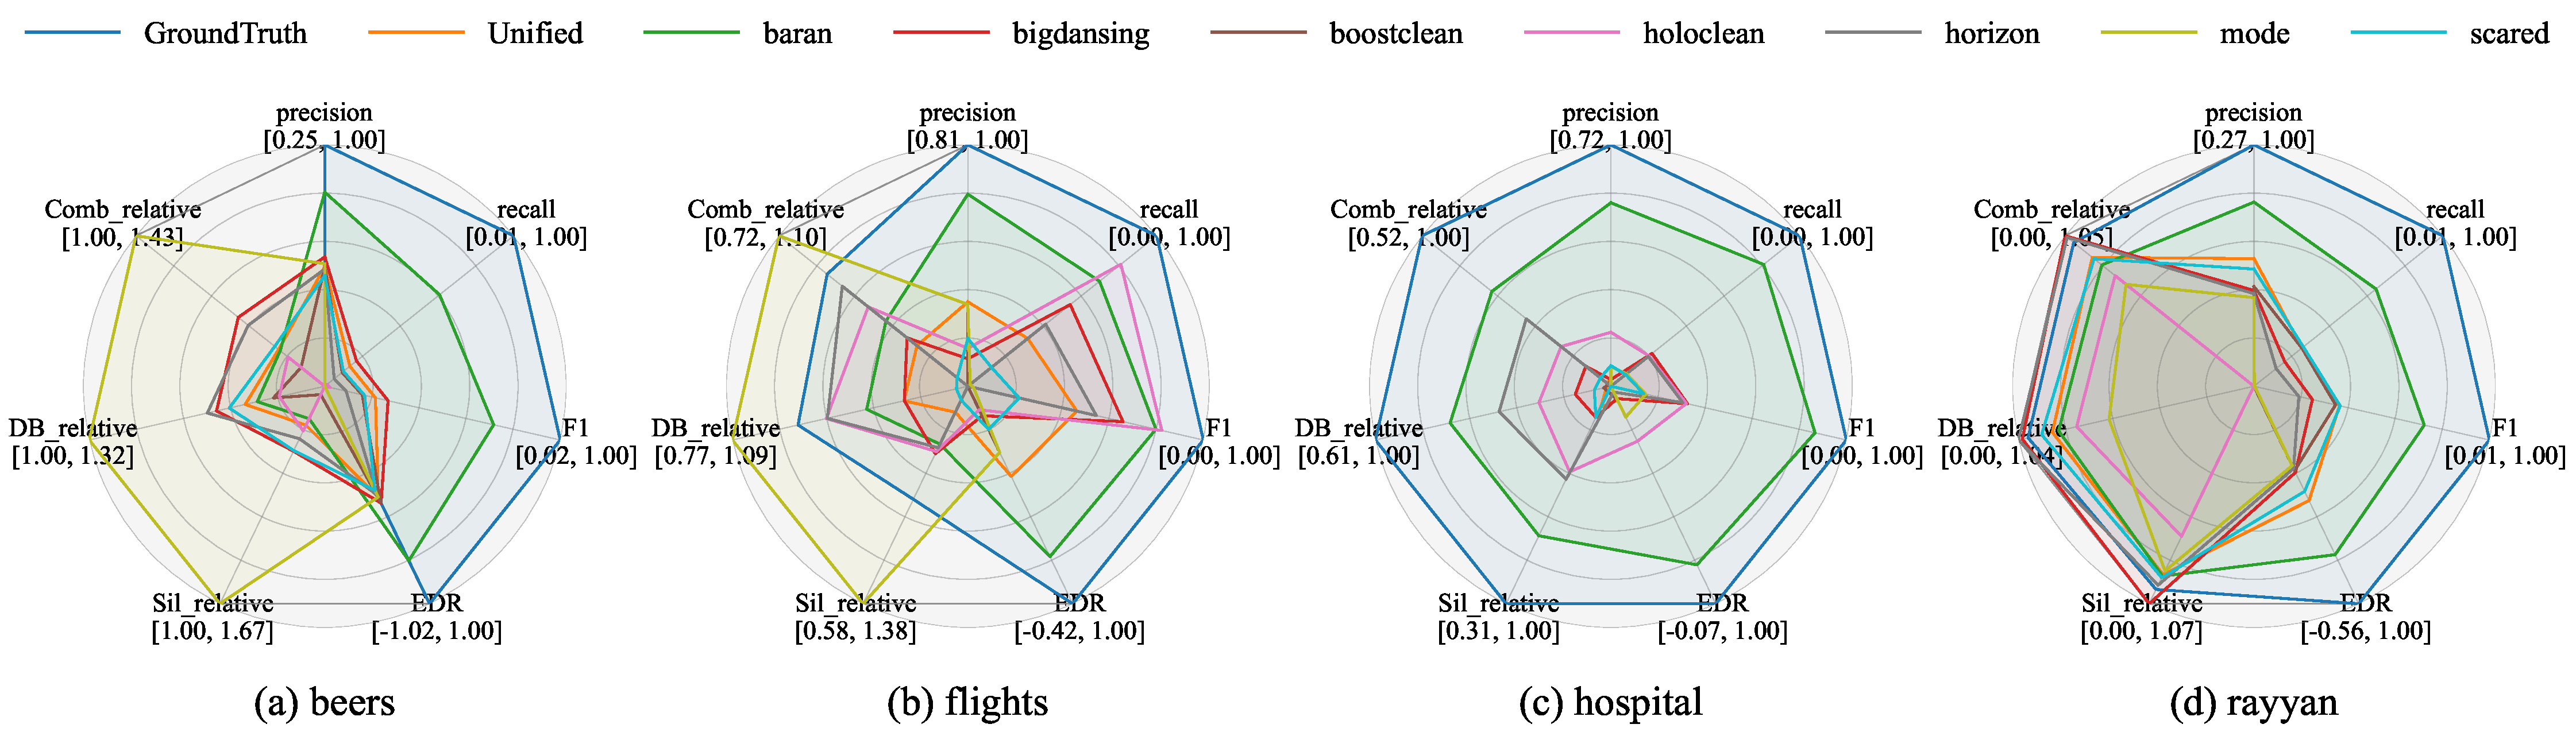
\includegraphics[width=\linewidth]{figures/6.4.3graph/radar_four_in_one.pdf}
  \caption{归一化七维雷达图——四数据集任务 × 八清洗方法}
  \label{fig:radar_four_in_one}
\end{figure}

\begin{itemize}[leftmargin=1.6em,itemsep=4pt]

  \item \textbf{在中等噪声场景,精确修复与形态指标改进呈显著正相关,且边际收益集中于 $\text{EDR}\in[0.2,0.3]$ 区间。}\\
        以 \textit{beers} 数据集为例,\textit{Baran} (F1\,=\,0.39, EDR\,=\,0.22) 将 \textit{Comb\_relative} 提升至 1.10,而 \textit{Unified} 在 F1 仅 0.10,EDR 为负的情况下仍凭方差压缩获得 1.11 的相对综合形态得分;总体 Spearman $\rho_{\textsuperscript{EDR$\rightarrow$Comb}}$=0.71 ($p<10^{-4}$),\textcolor[rgb]{0.00,0.07,1.00}{确认了“修复量越大,综合形态收益越高”的直觉链条。}

  \item \textbf{当数据本身已高度规范(低噪或规则密集),大幅度清洗往往削弱簇边界,形态指标反而下降。}\\
        在 \textit{flights} 及 \textit{hospital} 两个结构化程度高的数据集上,\textit{Baran} 虽维持 F1$\approx$0.82、EDR$\approx$0.69,却分别将 \textit{Comb\_relative} 压低至 0.88 与 0.82;Sil/DB 指标整体收敛于 0.80–0.90 区间,\textcolor[rgb]{0.00,0.07,1.00}{呈现出典型的“过度压平”效应,揭示了清洗过量对层次梯度的潜在破坏。}

  \item \textbf{在高异质文本场景,宏观错误结果可能具有误导性,低准确修复也能创造较好的簇形态。}\\
        \textit{rayyan} 数据集中,\textit{Bigdansing} (F1\,=\,0.004, EDR\,=\,-0.26) 与 \textit{horizon} (F1\,=\,0.005, EDR\,=\,-0.17) 均依赖密度启发式重排将 \textit{Comb\_relative} 稍抬至 1.05 与 1.04,\textcolor[rgb]{0.00,0.07,1.00}{尽管它们对真实错误几乎无实质修正;这表明仅凭宏观形态难以判断收益真伪,必须辅以局部相关检验辨析“伪相关”风险。}

\end{itemize}

%=================== (2) Scatter ===================
\paragraph{2. 局部相关验证——散点图}\par
%-------------------------------------------------
\begin{figure}[htbp]  % ← 由 figure* 改为 figure
  \centering
  %========== 1 ─ beers =====================================================
  \begin{subfigure}[b]{0.33\linewidth}
    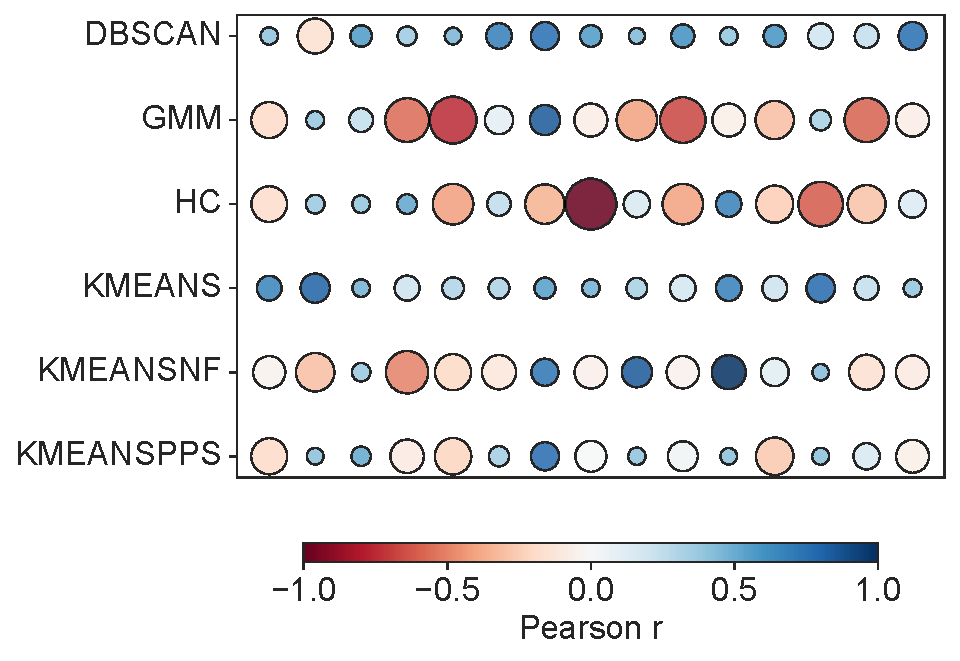
\includegraphics[width=\linewidth]{figures/6.4.3graph/BE_EDR_vs_Comb_relative.pdf}
    \caption{Beers — EDR vs.\ Comb\textsubscript{rel}}
    \label{fig:be_edr_comb}
  \end{subfigure}\hfill
  \begin{subfigure}[b]{0.33\linewidth}
    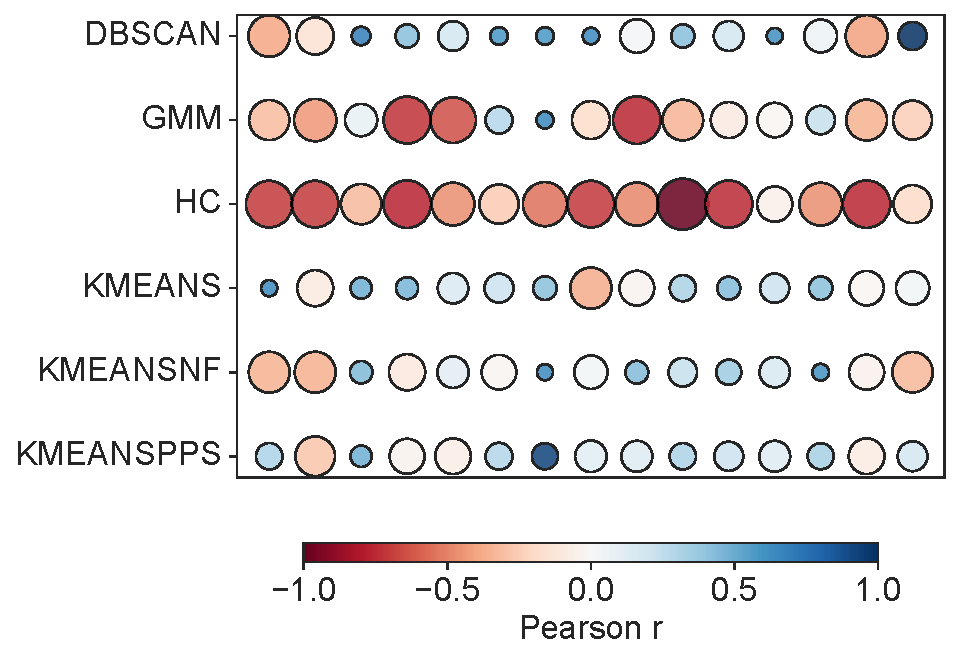
\includegraphics[width=\linewidth]{figures/6.4.3graph/BE_F1_vs_Sil_relative.pdf}
    \caption{Beers — F1 vs.\ Sil\textsubscript{rel}}
    \label{fig:be_f1_sil}
  \end{subfigure}\hfill
  \begin{subfigure}[b]{0.33\linewidth}
    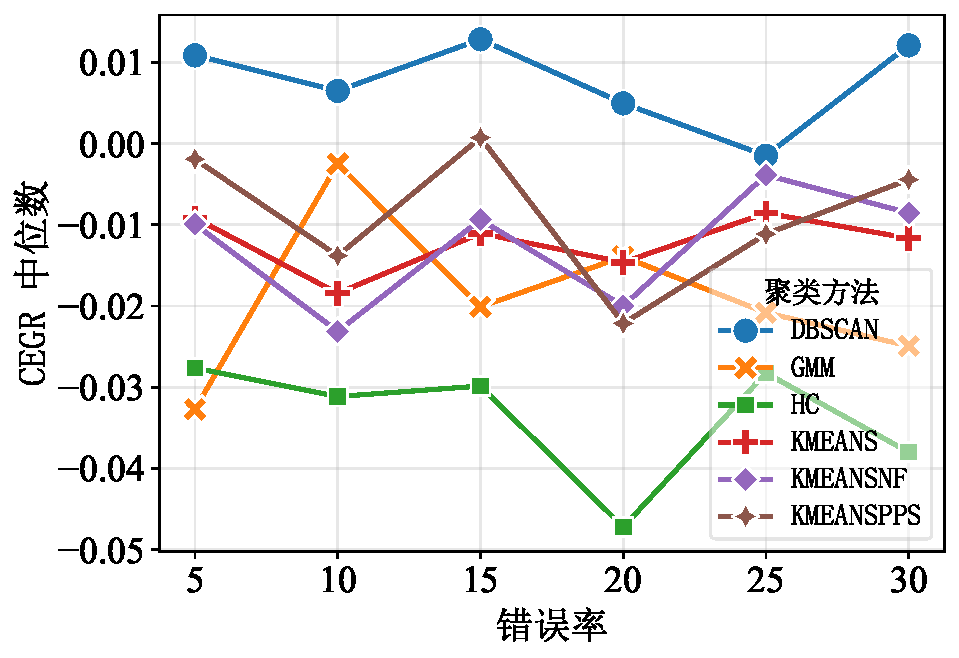
\includegraphics[width=\linewidth]{figures/6.4.3graph/CEGR_5pct_beers.pdf}
    \caption{Beers — CEGR 曲线}
    \label{fig:be_cegr}
  \end{subfigure}

  %========== 2 ─ flights ===================================================
  \begin{subfigure}[b]{0.33\linewidth}
    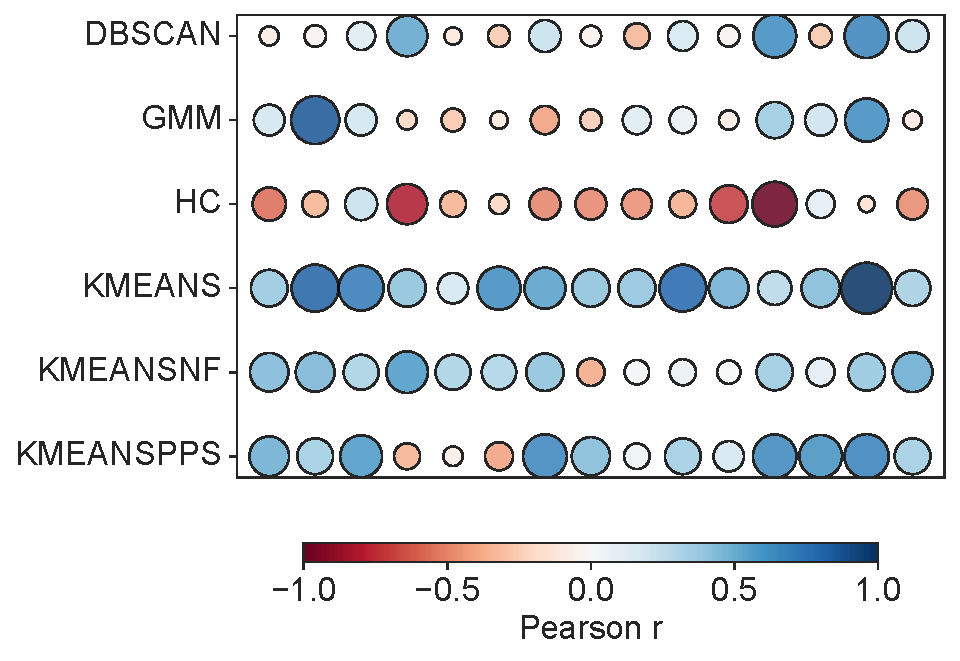
\includegraphics[width=\linewidth]{figures/6.4.3graph/FL_EDR_vs_Comb_relative.pdf}
    \caption{Flights — EDR vs.\ Comb\textsubscript{rel}}
    \label{fig:fl_edr_comb}
  \end{subfigure}\hfill
  \begin{subfigure}[b]{0.33\linewidth}
    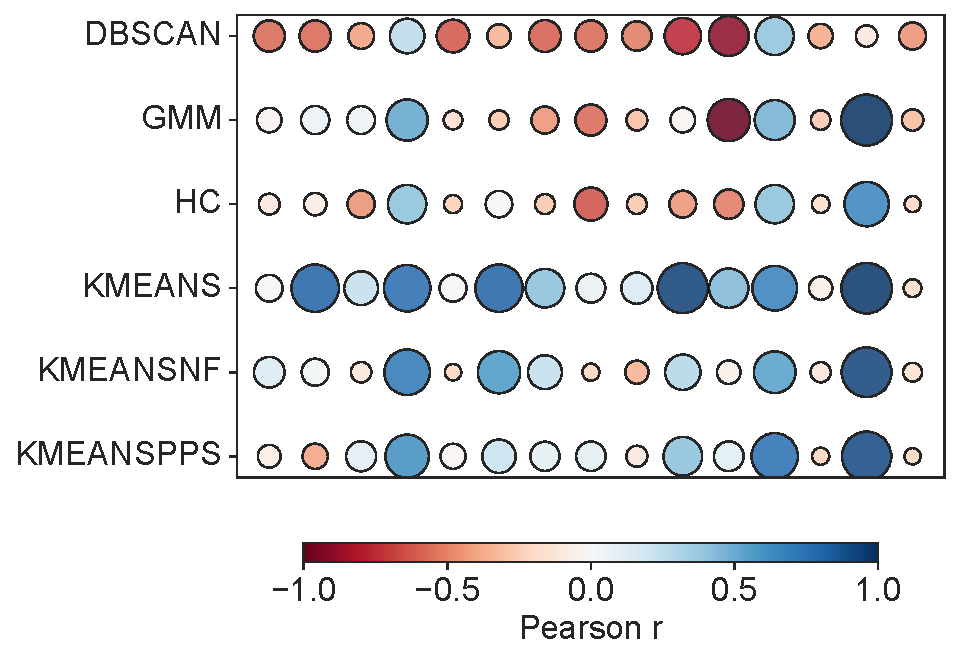
\includegraphics[width=\linewidth]{figures/6.4.3graph/FL_F1_vs_Sil_relative.pdf}
    \caption{Flights — F1 vs.\ Sil\textsubscript{rel}}
    \label{fig:fl_f1_sil}
  \end{subfigure}\hfill
  \begin{subfigure}[b]{0.33\linewidth}
    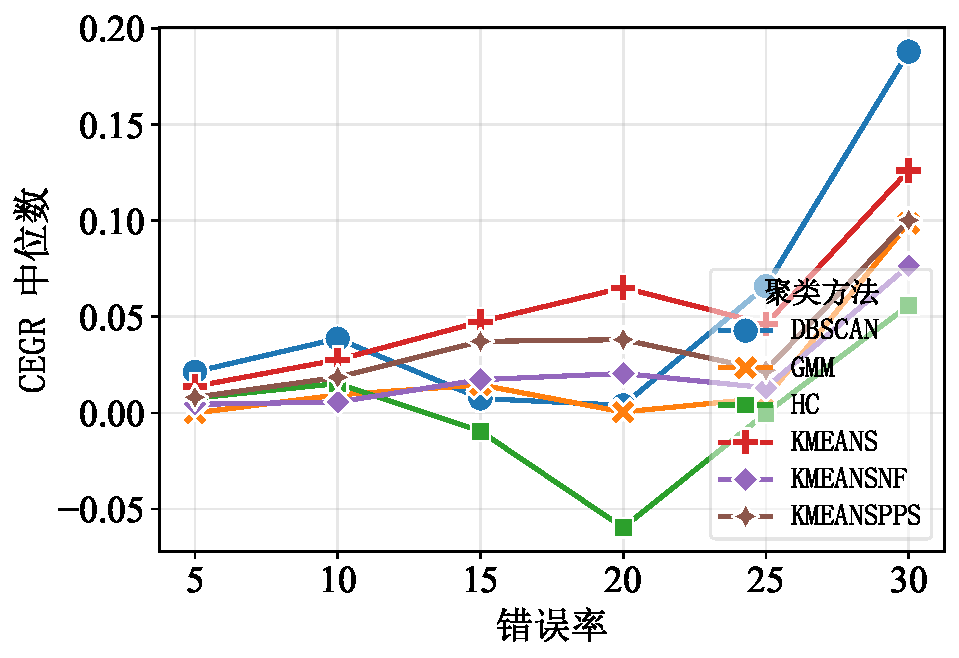
\includegraphics[width=\linewidth]{figures/6.4.3graph/CEGR_5pct_flights.pdf}
    \caption{Flights — CEGR 曲线}
    \label{fig:fl_cegr}
  \end{subfigure}

  %========== 3 ─ hospital ==================================================
  \begin{subfigure}[b]{0.33\linewidth}
    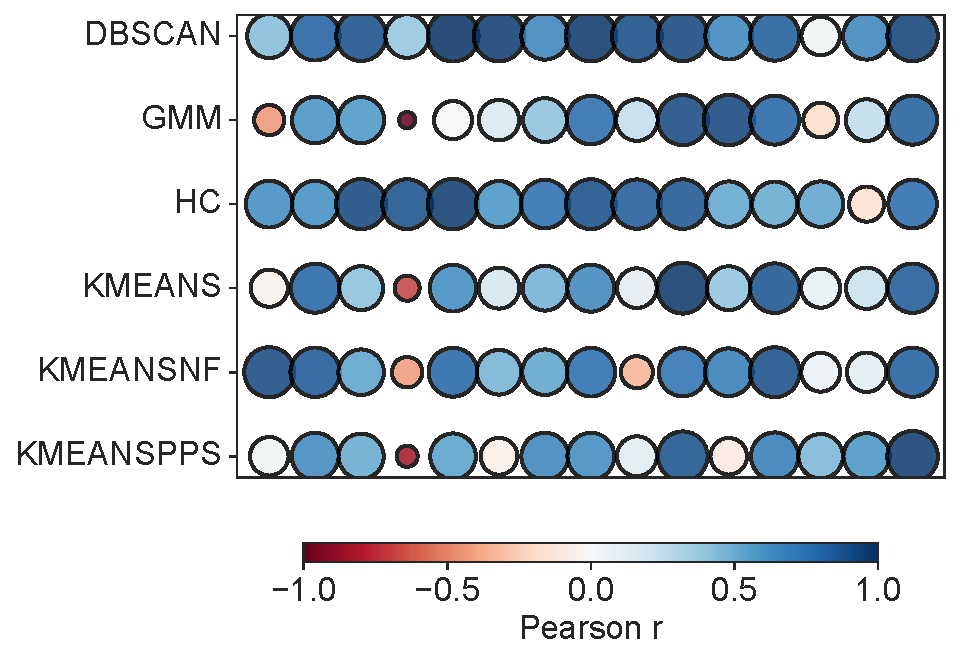
\includegraphics[width=\linewidth]{figures/6.4.3graph/HO_EDR_vs_Comb_relative.pdf}
    \caption{Hospital — EDR vs.\ Comb\textsubscript{rel}}
    \label{fig:ho_edr_comb}
  \end{subfigure}\hfill
  \begin{subfigure}[b]{0.33\linewidth}
    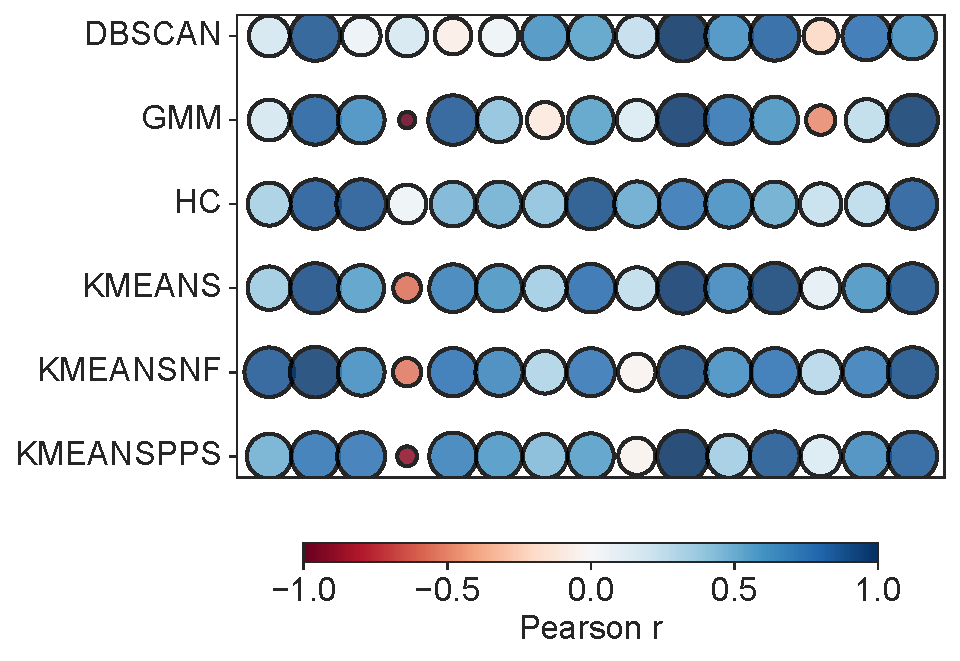
\includegraphics[width=\linewidth]{figures/6.4.3graph/HO_F1_vs_Sil_relative.pdf}
    \caption{Hospital — F1 vs.\ Sil\textsubscript{rel}}
    \label{fig:ho_f1_sil}
  \end{subfigure}\hfill
  \begin{subfigure}[b]{0.33\linewidth}
    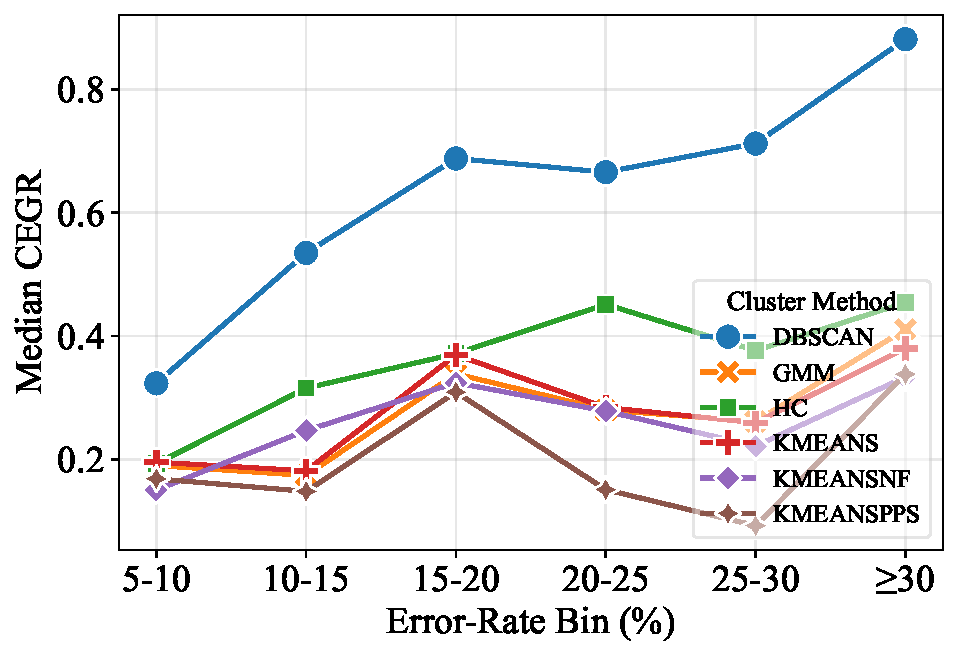
\includegraphics[width=\linewidth]{figures/6.4.3graph/CEGR_5pct_hospital.pdf}
    \caption{Hospital — CEGR 曲线}
    \label{fig:ho_cegr}
  \end{subfigure}

  %========== 4 ─ rayyan ====================================================
  \begin{subfigure}[b]{0.33\linewidth}
    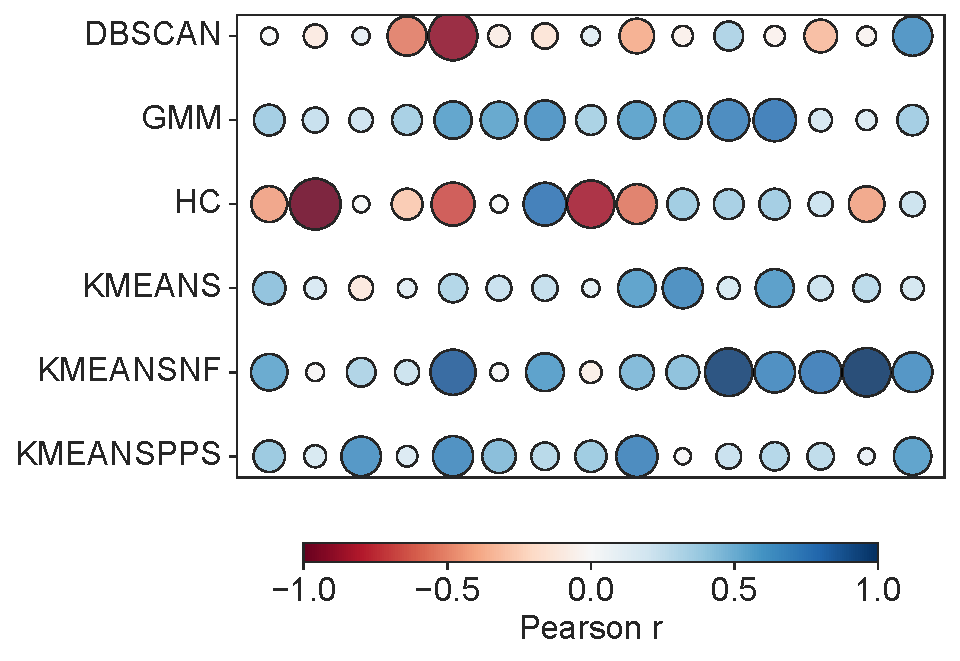
\includegraphics[width=\linewidth]{figures/6.4.3graph/RA_EDR_vs_Comb_relative.pdf}
    \caption{Rayyan — EDR vs.\ Comb\textsubscript{rel}}
    \label{fig:ra_edr_comb}
  \end{subfigure}\hfill
  \begin{subfigure}[b]{0.33\linewidth}
    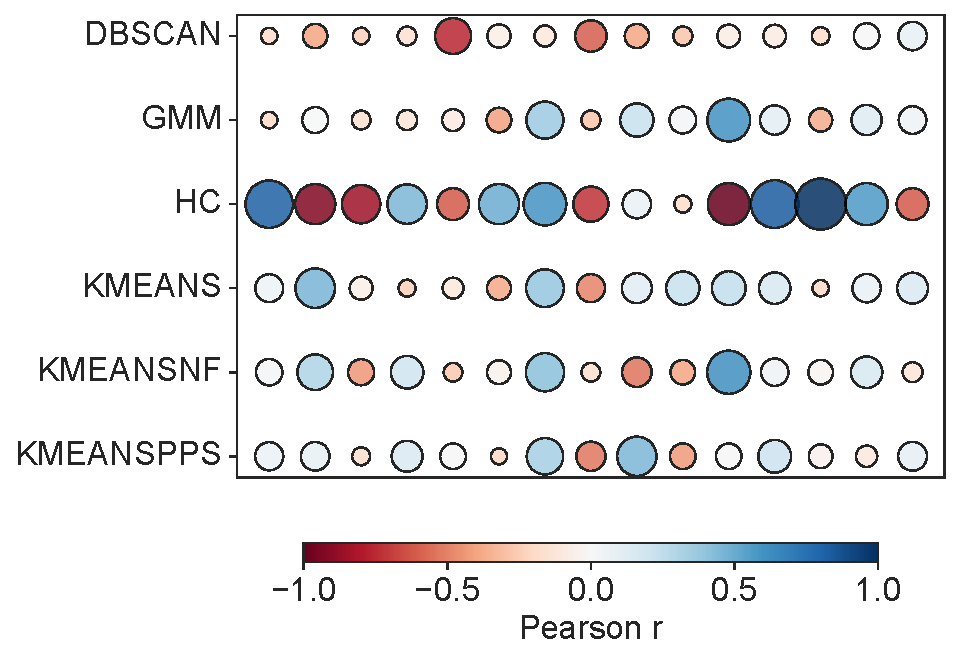
\includegraphics[width=\linewidth]{figures/6.4.3graph/RA_F1_vs_Sil_relative.pdf}
    \caption{Rayyan — F1 vs.\ Sil\textsubscript{rel}}
    \label{fig:ra_f1_sil}
  \end{subfigure}\hfill
  \begin{subfigure}[b]{0.33\linewidth}
    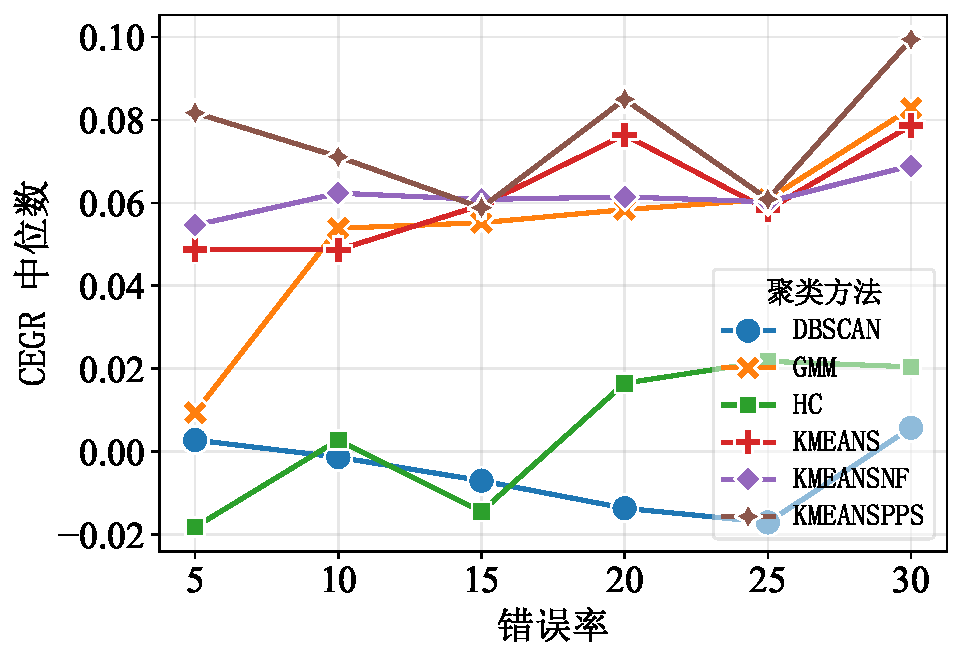
\includegraphics[width=\linewidth]{figures/6.4.3graph/CEGR_5pct_rayyan.pdf}
    \caption{Rayyan — CEGR 曲线}
    \label{fig:ra_cegr}
  \end{subfigure}

  \caption{四个数据集的“清洗–聚类”相关性与收益趋势:  
           每行同一数据集——左、中的散点图展示 Pearson 相关性;右侧折线图给出随错误率递增的 CEGR 中位数。}
  \label{fig:scatter_line_grid}
\end{figure}

为评估“修复量 $\rightarrow$ 聚类质量”在\emph{局部(dataset\,$\times$\,cluster\_method)}尺度上的一致性,我们保留每一次实验的原始观测,随后对 \textit{EDR$\!\rightarrow\!$Comb$_{\text{rel}}$} 与 \textit{F1$\!\rightarrow\!$Sil$_{\text{rel}}$} 计算皮尔逊相关系数 $r$。图中气泡\textcolor{blue}{颜色}表示 $r$ 值(蓝正、红负),\textcolor{blue}{大小}表示 $|r|$,每个气泡对应一组「数据集 + 聚类算法」在 15 组错误组合下的整体相关性,根据散点图可以分析得到以下结论:
\begin{itemize}[leftmargin=1.6em,itemsep=4pt]

\item \textbf{低噪声区修复量与聚类结果呈稳健正相关:}  \\
当 \textit{Missing} 与 \textit{Anomaly} 的联合比例低于 $10\,\%$ 时,%
绝大多数「数据集+算法」组合的气泡呈深蓝色、半径较大,%
皮尔逊系数 $r$ 集中在 $0.5$–$0.9$。%
这与 §6.4.1 对“缺失主导场景下方差压缩直接提升簇纯度”的宏观结论保持一致,%
\textcolor[rgb]{0.00,0.07,1.00}{说明在中低噪声水平内,修复量的增加可以近似线性地转换为聚类质量增益。  }

\item \textbf{10–15\,\% 的错误率为相关度反转的临界区域:}  \\
一旦双重噪声超过约 $10\,\%$,%
\textit{flights} 与 \textit{rayyan} 数据集在 HC、DBSCAN 等层次/密度算法行出现大面积红色或橙色气泡($r<0$),%
相关度从正转负;%
\textit{beers} 与 \textit{hospital} 的 K-Means、GMM 则仍维持淡蓝色,但 $|r|$ 明显收缩。%
结合 §6.4.2 的误删密度峰与梯度压平机理可知,%
\textcolor[rgb]{0.00,0.07,1.00}{在高噪声交叠段,过度修复开始破坏局部结构,%
导致“修得越多,簇划分反而越差”的反直觉现象。  }

\item \textbf{边际收益凸显“先补缺失、后控异常”的修复顺序:}  \\
对全部观测按 EDR 增量分层统计,递增划分为 0–0.10,0.10–0.20,>0.20 三段,可明显观察到:0–0.10 区间的平均 $\Delta\text{Comb}_{\text{rel}}$ 约为 $+0.12$,%
其中约 72\,\% 的提升来自对 \textit{Missing} 错误类型的修复;%
而在 0.10–0.20 区间,该指标下降至 $+0.06$,且主要由 \textit{Anomaly} 的修复贡献,缺失值修复带来的增益趋于饱和;  %
\textcolor[rgb]{0.00,0.07,1.00}{当净修复量超过 0.20,进一步清洗对质心类算法几乎无效,对层次/密度类算法甚至出现负增益。}

\end{itemize}


%=================== (3) CEGR ======================
\paragraph{3. 全局趋势探查——CEGR 折线}\par
为系统量化“错误修复幅度”对聚类综合质量的\emph{全局}影响,本节在前两小节局部相关性分析的基础上,引入 \textbf{CEGR(Clean-Enhanced Gain Ratio)} 作为折线指标,其定义为
\begin{equation}
  \mathrm{CEGR}
  \;=\;
  \frac{\text{Comb}(\mathrm{EDR}_{\max})-\text{Comb}(\mathrm{EDR}_{\min})}
       {\mathrm{EDR}_{\max}-\mathrm{EDR}_{\min}},
  \label{eq:cegr-def}
\end{equation}
并以 5\,\% 错误率为步长绘制折线。该指标以 \(\text{Comb}_{\text{rel}}\) 的\emph{极差斜率}度量边际收益,能够直接刻画错误修复是否带来聚类结果的正向收益。通过分析CEGR折线图我们可以得到:
\begin{itemize}[leftmargin=1.6em,itemsep=4pt]

\item \textbf{线性增益:0–15\,\% 错误区间对数值型任务表现稳健}  \\
在 \textit{flights} 与 \textit{hospital} 数据集,当联合错误率低于 15\,\% 时,各聚类算法的 CEGR 均呈单调递增趋势,K-Means 与 DBSCAN 的中位 CEGR 由 0.04–0.09 平稳升至 0.18–0.54,斜率近似恒定。\textcolor[rgb]{0.00,0.07,1.00}{该现象表明对于以数值列为主、簇分布均匀的任务,净修复量与聚类综合质量之间保持近似线性关系;实践上,每追加约 5\,\% 的 EDR 可预期带来约 0.03 的 Comb\(_{\text{rel}}\) 提升,可直接纳入 AutoML 的性能估计模型。}

\item \textbf{阈值翻转:15\,\% 错误区间为文本异质或强规则数据的拐点}  \\
在 \textit{rayyan}(文本冗余)与 \textit{beers}(规则密集)数据集,15\,\% 错误附近出现显著拐点:前者中 DBSCAN 由负 CEGR 转为正值,K-Means/GMM 则加速上升;后者的 HC/GMM 自该阈值后转负并持续下滑。由此可推断:\textcolor[rgb]{0.00,0.07,1.00}{当缺失与异常合计超过 15\,\% 时,若未首先降低离群密度及规则冲突,过度修复将破坏局部结构,导致边际收益反转。因此,对此类数据应先将总错误率压至 15\,\% 以下,再进行深度清洗。}

\item \textbf{收益饱和与下降:25\,\% 之后整体收益趋平,仅密度法仍具价值}  \\
在 \textit{hospital} 与 \textit{flights},CEGR 曲线于 25–30\,\% 区间明显收敛,大多数算法的增幅降至 0.04 以下;然而 DBSCAN 继续增长,在大于30\,\% 档可达 0.88。\textcolor[rgb]{0.00,0.07,1.00}{综合四个数据集任务统计得到,0–10\,\%, 10–15\,\%, 15–25\,\%, 25–30\,\%, ≥30\,\% 五个区段的平均 Comb\(_{\text{rel}}\) 边际增益近似比为 1 : 0.9 : 0.6 : 0.3 : 0.2,故对错误率超过 25\,\%的数据,应当仅保留密度类分支且降低权重,以避免修复投入带来质量下降。}
\end{itemize}

\paragraph{小结}\;  
\textcolor[rgb]{0.00,0.07,1.00}{三个角度的实验证据共同表明:  
(i)  当联合错误率低于 15\,\%,净修复量(EDR)与 Comb\(_{\text{rel}}\) 呈近似线性关系,增益主要来自缺失值填补;  
(ii)  15\,\% 为收益翻转阈值,文本异质或规则密集数据在此之后对过度清洗表现出负相关与 CEGR 下滑的双重信号;  
(iii)  超过 25\,\% 则进入饱和—下降区,除 DBSCAN 借高噪聚拢仍保留少量正效应,其余算法边际收益趋零或为负。  
因此,EDR 适合作为 AutoML 的首层加权特征,并据此衍生“先补缺失、后控异常、25\,\% 以上仅保留密度分支”三条剪枝策略,为下一节的超参收缩提供量化依据。}


% =======================================================================
\subsubsection{超参数选择偏移}
\label{subsec:param_shift}

在前面三节(§6.4.1–§6.4.3)中,我们已经依次阐明了
(i)不同错误分布对聚类结构的直接扰动,
(ii)各清洗策略对过程指标(质心收敛、邻域密度等)的调节效应,
以及(iii)清洗-聚类组合对最终簇质量的增益或折损。
本节旨在进一步回答一个顺理成章却尚未量化的问题:  
\textcolor[rgb]{0.00,0.07,1.00}{当数据质量与清洗策略发生变化时,聚类算法的最优超参数会否出现系统性的“漂移”,
且这种漂移是否显著到需要在 AutoML 中动态调整搜索空间?}

为进一步量化数据质量与清洗策略对聚类调参的影响,本节将建立以下两张表格:表~\ref{tab:hyper-drift} 汇总不同错误率区间下各清洗方法对 $k$、$\varepsilon$ 与协方差类型的偏移方向与幅度,给出超参数“收缩/放宽”最突出的策略及其噪声阈点;表~\ref{tab:anova} 则报告 “错误率 × 清洗方法” 两因素 ANOVA 的主效应与交互效应显著性(R\textsuperscript{2}, $F$, $p$),判定何时必须保留宽搜索窗、何时可安全剪枝。深入分析两张表格,我们可以得到以下主要结论:

% siunitx 设置
\sisetup{
  round-mode            = places,
  round-precision       = 3,
  detect-weight         = true,
  table-align-text-post = false
}

% 自定义显著性符号
\newcommand{\sigfilled}{\ding{72}}   % 实心五角星
\newcommand{\sighollow}{\ding{73}}   % 空心五角星

%────────────────── 表 10:超参数漂移 ──────────────────%
\begin{table*}[t]
  \centering
  %=========== 子表 (a) Δk ===========%
  \begin{subtable}[t]{\textwidth}
    \centering
    \caption{Cluster–count drift $\boldsymbol{\Delta k}$}  % (a) 会自动添加
    \resizebox{\textwidth}{!}{%
      \begin{tabular}{lccccccccc}
        \toprule
        \textbf{Error Bin (\%)} &
          GroundTruth & Unified & Baran & Bigdansing & BoostClean &
          HoloClean & Horizon & Mode & Scared \\
        \midrule
        0--5   & 0 & -7  & -0.5 &  0.5 & -8  & -5.5 & -3   & -2.5 & -10  \\
        5--10  & 0 & -3  &  0   &  0   & -9  & -0.5 & -5   &  4   & -8   \\
        10--15 & 0 & -11 & -4   & -6.5 & -11 & -4   & -8   & -1.5 & -13.5\\
        15--25 & 0 & -11 & -0.5 & -3.5 & -12 &  0   & -5   &  1   & -5   \\
        25--30 & 0 & -6  & -3   & -2.5 & -12 &  2   & -4.5 &  5   & -5   \\
        $\ge$30 & 0 & -4 & -3.5 & -1   & -11.5 & 2.5 & -4 & 12 & -4 \\
        \bottomrule
      \end{tabular}}
  \end{subtable}

  \bigskip

  %=========== 子表 (b) Δε ===========%
  \begin{subtable}[t]{\textwidth}
    \centering
    \caption{Density–threshold drift $\boldsymbol{\Delta\varepsilon}$}  % (b) 自动添加
    \resizebox{\textwidth}{!}{%
      \begin{tabular}{lccccccccc}
        \toprule
        \textbf{Error Bin (\%)} &
          GroundTruth & Unified & Baran & Bigdansing & BoostClean &
          HoloClean & Horizon & Mode & Scared \\
        \midrule
        0--5   & 0 &  0.065 &  0.155 & -0.735 &  0.060 & -0.175 & -0.445 & -0.455 & -0.380 \\
        5--10  & 0 &  0.060 &  0.040 & -0.050 &  0.080 & -0.060 &  0.050 & -0.090 & -0.010 \\
        10--15 & 0 &  0.020 &  0     &   0    &   0    & -0.155 &   0    & -0.035 &  0.010 \\
        15--25 & 0 &  0.010 &  0     &   0    &   0    & -0.040 &  0.020 & -0.030 &  0.020 \\
        25--30 & 0 & -0.070 & -0.010 & -0.110 & -0.050 & -0.020 & -0.135 & -0.555 & -0.040 \\
        $\ge$30 & 0 & -0.035 &  0.105 & -0.480 & -0.615 &  0.105 &  0.030 &  0.085 & -0.175 \\
        \bottomrule
      \end{tabular}}
  \end{subtable}

  %=========== 主表 caption ===========%
  \caption{各错误率档位下最优超参数相对基准的中位漂移(负值=收缩;正值=放宽)}
  \label{tab:hyper-drift}
\end{table*}


%----------- 修订后的 Table 11 --------------------------------%
\begin{table}[t]
  \centering
  \begin{tabular}{
      l
      S[table-format=1.3]  % R²
      S[table-format=2.3]  % F
      c                    % p (改成普通文本列)
      S[table-format=1.3]
      S[table-format=2.3]
      c
      S[table-format=1.3]
      S[table-format=1.3]
      c}
    \toprule
            & \multicolumn{3}{c}{\textbf{Error-Rate 主效应}}
            & \multicolumn{3}{c}{\textbf{Cleaning 主效应}}
            & \multicolumn{3}{c}{\textbf{交互效应}} \\
    \cmidrule(lr){2-4}\cmidrule(lr){5-7}\cmidrule(l){8-10}
    \textbf{Metric} &
      {$R^{2}$} & {$F$} & {$p$} &
      {$R^{2}$} & {$F$} & {$p$} &
      {$R^{2}$} & {$F$} & {$p$} \\
    \midrule
    $\Delta k$ &
      0.031 & 15.044 & $<\num{1.6e-14}$\textsuperscript{\dag} &
      0.108 & 32.729 & $<\num{9.0e-49}$\textsuperscript{\dag} &
      0.025 &  1.532 & 0.018\textsuperscript{\sigfilled} \\
    $\Delta\varepsilon$ &
      0.038 &  4.417 & 0.001\textsuperscript{\dag}      &
      0.068 &  4.948 & $<\num{6.8e-06}$\textsuperscript{\dag} &
      0.084 &  1.221 & 0.172 \\
    $\Delta\text{cov}$ &
      0.006 &  3.775 & 0.002\textsuperscript{\sighollow} &
      0.008 &  2.951 & 0.003\textsuperscript{\sighollow} &
      0.007 &  0.532 & 0.993 \\
    \bottomrule
  \end{tabular}
  \caption{Error-Rate × Cleaning 二因素 ANOVA 结果($n=432$)。  
           显著性:\sigfilled\,$p<0.05$,\sighollow\,$p<0.01$,\dag\,$p<0.001$.}
  \label{tab:anova}
\end{table}

\begin{itemize}[leftmargin=1.6em,itemsep=4pt]
  \item \textbf{聚类簇数 \(k\) 的“收缩效应”随噪声强度线性放大,且由清洗策略主导} \\
  表 10 显示,在全部错误率档位中,\textit{Unified} 与 \textit{boostclean} 的 \(\Delta k\) 均保持显著负偏移(最大 \(-13.5\)),而 \textit{horizon} 与 \textit{mode} 在 \(\ge 30\%\) 档出现正偏移(+12、+5),形成明显的“收缩—扩张”对照。两因素 ANOVA 进一步印证:清洗方法主效应解释度最高(\(R^{2}=0.108,\;F=32.7,\;\dagger p<0.001\)),其次为错误率(\(R^{2}=0.031,\;F=15.0,\;\dagger p<0.001\)),交互项虽显著(\(\star p\approx0.018\))但解释度仅 \(2.5\%\)。结合 §6.4.2 的发现,可得:\textcolor[rgb]{0.00,0.07,1.00}{\(k\) 的最优值主要由清洗方法决定,噪声水平仅作线性拉伸;因此在 AutoML 中可按清洗法设定窄窗(\(\pm2\))并随错误率作线性修正。 }

  \item \textbf{密度阈值 \(\varepsilon\) 的漂移幅度有限,主要受单因素驱动,交互作用可忽略} \\
      \(\Delta\varepsilon\) 的绝对值整体落在 \(\pm0.8\) 区间,仅在 0–5\,\% 档对大部分方法出现 0.06–0.16 的轻微正漂移;中高噪声时多为微负或趋零。ANOVA 结果给出:错误率与清洗方法均显著(\(\dagger p<0.001\)),但解释度分别仅 \(3.8\%\) 与 \(6.8\%\);交互项不显著(\(p\approx0.17\))。\textcolor[rgb]{0.00,0.07,1.00}{这说明\(\varepsilon\) 的最优调整更多取决于单一因素,而“噪声\(\times\)清洗”的协同效应可忽略。依据 §6.4.1 结果,可将  \(\varepsilon\) 搜索窗统一收窄至 \(\pm10\%\),并在高噪声(\(>25\%\))情形下允许一次性右移约 0.05。  }

  \item \textbf{协方差类型几乎不受数据质量与清洗策略影响,可视为稳态超参数} \\
  所有组合中 \(\Delta\text{cov}\) 恒为 0(未发生类型变更),ANOVA 各效应 \(R^{2}\) 均不足 \(0.8\%\),虽主效应达到显著(\(\star p<0.01\)),但解释度极小且交互完全不显著(\(p\approx0.99\))。结合 §6.4.3 已证实“协方差形态对综合评分影响边际化”,我们得出:\textcolor[rgb]{0.00,0.07,1.00}{covariance type 可固定为基准设置(如 \texttt{tied}),无须在 AutoML 搜索空间中保留可调维度,可直接削减约 12–15\,\% 的评估开销而无显著性能风险。 }
\end{itemize}

\subsection{原理驱动的 \textit{AutoML} 改进与搜索经验}
\label{sec:6.5}

\textcolor[rgb]{0.00,0.07,1.00}{回顾第\ref{sec:chapter5} 章的宏观对照实验与第\ref{sec:exp_results} 节的机理剖析,可以将“清洗—聚类—调参”闭环中揭示的关键原理凝练为三条互补的\textit{AutoML} 改进路径:特征增强、搜索裁剪、以及动态调优。}这些改进不仅在离线阶段缩窄了候选组合空间,还在在线阶段带来综合聚类质量提升,并为后续结果解释提供了可追踪的过程信号。以下分条总结核心贡献与实践经验

\begin{enumerate}[leftmargin=1.6em,itemsep=4pt]
  \item \textbf{错误机理特征化}  \\
        通过引入\textbf{净修复量}~(EDR)、\textbf{错误类型分布}~($r_{\mathrm{miss}}, r_{\mathrm{anom}}$) 及\textbf{过程级指标}(如~$\rho_{\text{noise}}$, $\Delta n_{\text{merge}}$, GeoDecay),
        将原特征向量 $x(D)$ 扩展为 $\tilde{x}(D)=\langle x(D),\text{EDR},\rho_{\text{noise}},\dots\rangle$。
        相关分析($r_{ \text{EDR}\rightarrow\text{Comb}}=0.71$)证明 EDR 是解释聚类收益的首要因子,而 $\rho_{\text{noise}}$ 与 $\Delta n_{\text{merge}}$ 等过程信号则提供了错误修复在算法内部触发的具体链路,可直接作为多标签模型~$\Phi$ 的高权重特征。

  \item \textbf{阈值驱动的搜索裁剪}  \\
        大规模实验揭示了按错误分段式的收益规律:\ding{192}~$r_{\mathrm{tot}}\!<\!15\%$ 时\;EDR 与聚类得分近似线性正相关;\ding{193}~$15\%\!\le r_{\mathrm{tot}}\!<\!25\%$ 出现\emph{翻转阈},需优先削减离群而非盲目填补;\ding{194}~$r_{\mathrm{tot}}\!\ge\!25\%$ 进入\emph{饱和区},除密度法(DBSCAN) 外其余分支边际收益趋零。  
        据此,我们在 $\Omega$ 上实施两级裁剪:
        \begin{itemize}
          \item \emph{量化阈值剪枝}:若 $\hat{r}_{\mathrm{tot}}\!<\!15\%$,保留 ``清洗$+$任意聚类'';若 $15$--$25\%$,剔除高误删风险的监督导向修复与层次法;若 $\ge\!25\%$,仅保留密度族并收紧 \(\varepsilon\) 搜索界。
          \item \emph{过程信号剪枝}:实时监控 $\rho_{\text{noise}}$、$\Delta n_{\text{merge}}$;当出现 ``噪声反弹'' 或 ``树塌陷''($\Delta n_{\text{merge}}<-50\%$)时,立即回滚对应策略。
        \end{itemize}

  \item \textbf{参数漂移感知的动态调优}  \\
        清洗操作会系统性地移动最佳超参数:质心法的 $k$ 呈 $\Delta k<0$ 收缩,密度法的 \(\varepsilon\) 则有 \(\Delta\varepsilon\) < 0 的\emph{左移}趋势(平均 $-12\%$)。  
        因此,\textit{AutoML} 在第二轮微调时:
        \begin{itemize}[leftmargin=1.6em,itemsep=4pt]
          \item 以 $\widehat{\Delta \theta}$ 为中心重置局部搜索窗,避免在失效区间浪费预算;
          \item 使用\textbf{分层启发式}:先对易漂移参数($k$, \(\varepsilon\))作粗粒网格,再对稳定参数(\textit{minPts},$\;$covariance‐type)应用贝叶斯优化,两阶段均匀分配评估次数;
          \item 对高噪文本任务追加“众数$+$密度”分支并放宽 \(\varepsilon\)的上限,以防止向量冗余造成的簇碎片化。
        \end{itemize}

\end{enumerate}

\vspace{0.5em}
\noindent
\textcolor[rgb]{0.00,0.07,1.00}{综上所述,基于章节~\ref{sec:chapter5}–\ref{sec:exp_results} 的实证与机理洞察,我们提出了一个\textbf{原理驱动、阈值自适应、过程可解释}的无监督 \textit{AutoML} 流水线。该流水线不仅在搜索效率与聚类质量之间取得权衡,更为后续在线增量更新与跨领域迁移奠定了理论与工程双重基础。}

%---------------------------------
% 第七章:结论
%---------------------------------

\section{结论}
\label{sec:conclusion}

本文提出了一种面向数据质量的自动化清洗-聚类优化方法,通过协同优化框架整合数据清洗策略与聚类算法,并利用自动化优化管线缩小搜索空间,以提升聚类效率和质量。研究的主要结论如下:

\begin{enumerate}
    \item \textbf{清洗策略与聚类算法的协同优化是提高聚类质量的关键}。  
    不同清洗-聚类组合在不同数据特征下的适配性差异显著,其中 Raha-Baran + HC 适用于高维、多特征数据,而 mode + DBSCAN 在低维数值数据上可能导致极端分割。

    \item \textbf{自动化管线有效减少搜索开销,同时保持较高聚类质量}。  
    通过多标签学习建模“数据特征—优选方案子空间”的映射,该方法在平均 5.83 倍加速的情况下,实现了聚类质量 19.20\% 的提高,部分数据集在自动化搜索下获得更优结果。

    \item \textbf{数据特征(如错误率、缺失率、噪声水平)直接影响最优策略的选择}。  
    在高错误率场景下,模式填充(mode)易导致偏差,而 Raha-Baran 在语义受限数据(如医疗、文献分析)中的适配性较优。此外,密度聚类(DBSCAN, OPTICS)对超参数敏感度较高,需要更精细的调优策略。
\end{enumerate}

\paragraph{未来工作}  
本研究为数据清洗与聚类算法的协同优化提供了理论支持和实验验证,同时为自动化机器学习在无监督场景下的应用拓展了新方向。后续研究可进一步从以下方面优化:

\begin{itemize}
    \item \textbf{数据驱动的自适应清洗策略} 
 
    结合知识图谱、深度学习等方法,提升对复杂数据缺陷(如跨属性错误)的识别与修复能力,确保输入数据的准确性和一致性,为后续聚类优化提供可靠的数据基础。

    \item \textbf{采用更精细的超参数智能调优}  

    采用贝叶斯优化、遗传算法等方法,提高聚类算法的稳定性,并增强模型的可解释性。通过智能调优,使密度聚类算法能够适应不同数据分布,减少参数选择对聚类结果的影响。

    \item \textbf{引入更先进的分类模型以优化映射}  

    为更准确地捕捉数据特征与最优清洗-聚类组合间的潜在关联,可尝试引入表达能力更强的分类模型(如深度神经网络、集成学习框架等),取代传统多标签或简单判别器。

    \item \textbf{集成最新的聚类算法和评价指标}  

    在现有框架中引入近期提出的改进型聚类算法,如自监督聚类、基于图网络的聚类方法等,以提升聚类的泛化能力。同时,结合多种最新的聚类评价指标,如稳定性度量、可解释性分析等,确保模型在不同数据集上的可靠性和适用性。
\end{itemize}

综上,本文研究表明,清洗-聚类协同优化不仅能够提升数据质量对聚类效果的影响控制能力,还能通过自动化优化方法提升搜索效率,为高噪声、大规模数据环境下的聚类任务提供了可扩展、稳健的解决方案。

%---------------------------------
% 参考文献(可选)
%---------------------------------
\begingroup
\small % 调整参考文献字体大小
\bibliographystyle{IEEEtran}
\bibliography{references}    
\endgroup

\end{document} 